\documentclass[12pt]{extarticle}
\usepackage[paperwidth=18in,paperheight=8.5in]{geometry}
\usepackage{amsmath}
\usepackage{hyperref}
\usepackage{multirow}
\usepackage{pdfpages}
\usepackage[utf8]{inputenc}
\title{Kaon mixing: chiral and continuum extrapolations}
\author{R Mukherjee}
\date{\today}
\begin{document}
\maketitle
\tableofcontents
\clearpage
\begin{figure}
\centering
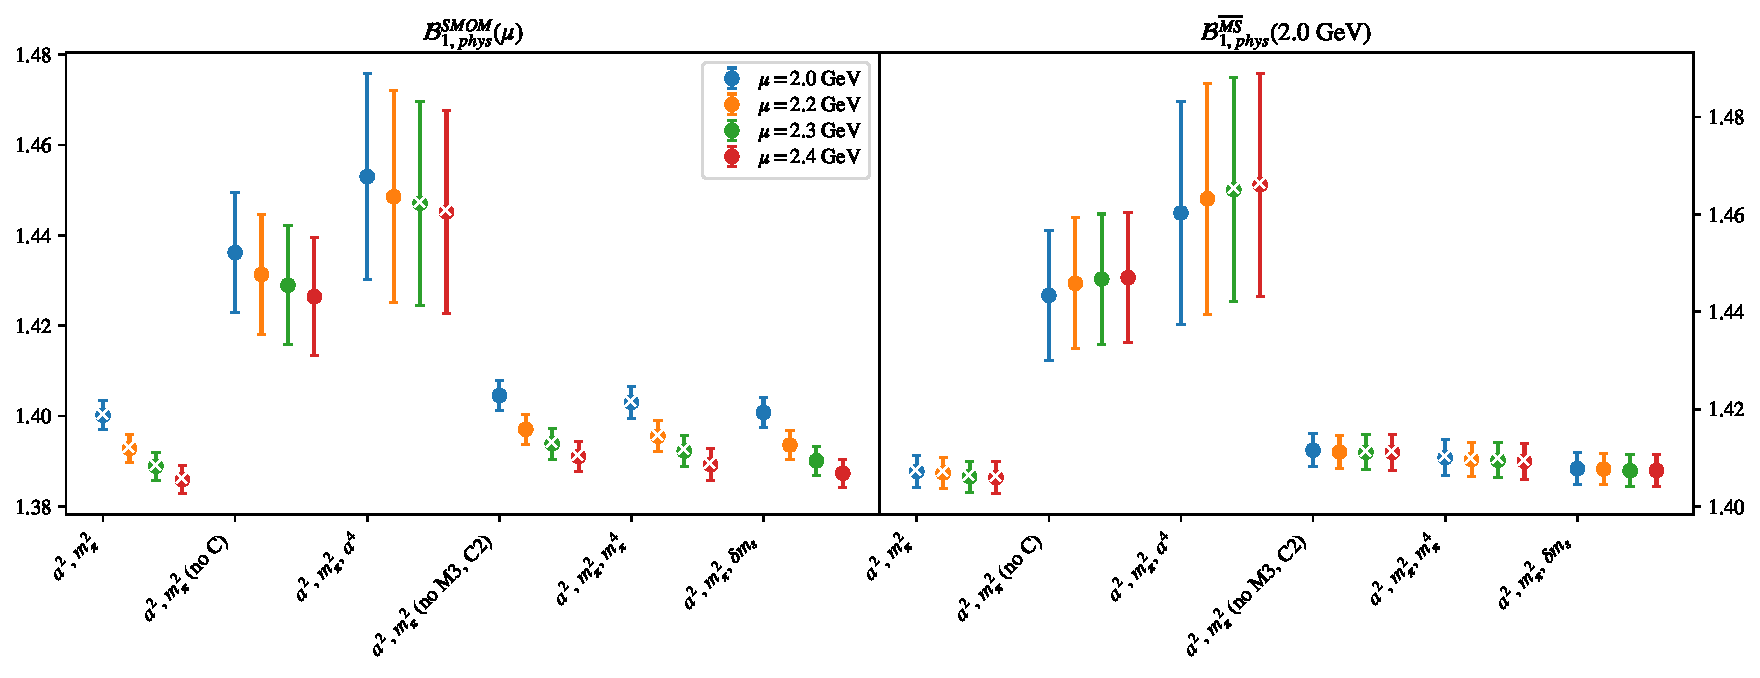
\includegraphics[page=1, width=1.1\textwidth]{VVpAA/NPR/fit_summary_bag.pdf}
\caption{$\mathcal{B}_{1}$\\(left) $\mathcal{B}_{phys}$ in RI/SMOM scheme from fit variations (fits with $p$-value $<0.05$ marked with ``$\times$"). \\(right) $\mathcal{B}_{phys}$ in $\overline{MS}$ computed using $\mathcal{B}^{\overline{MS}} = R^{\overline{MS}\leftarrow SMOM}(2.0)\sigma_{npt}(2.0,\mu) \mathcal{B}^{SMOM}(\mu)$.}
\end{figure}
\clearpage
\begin{figure}
\centering
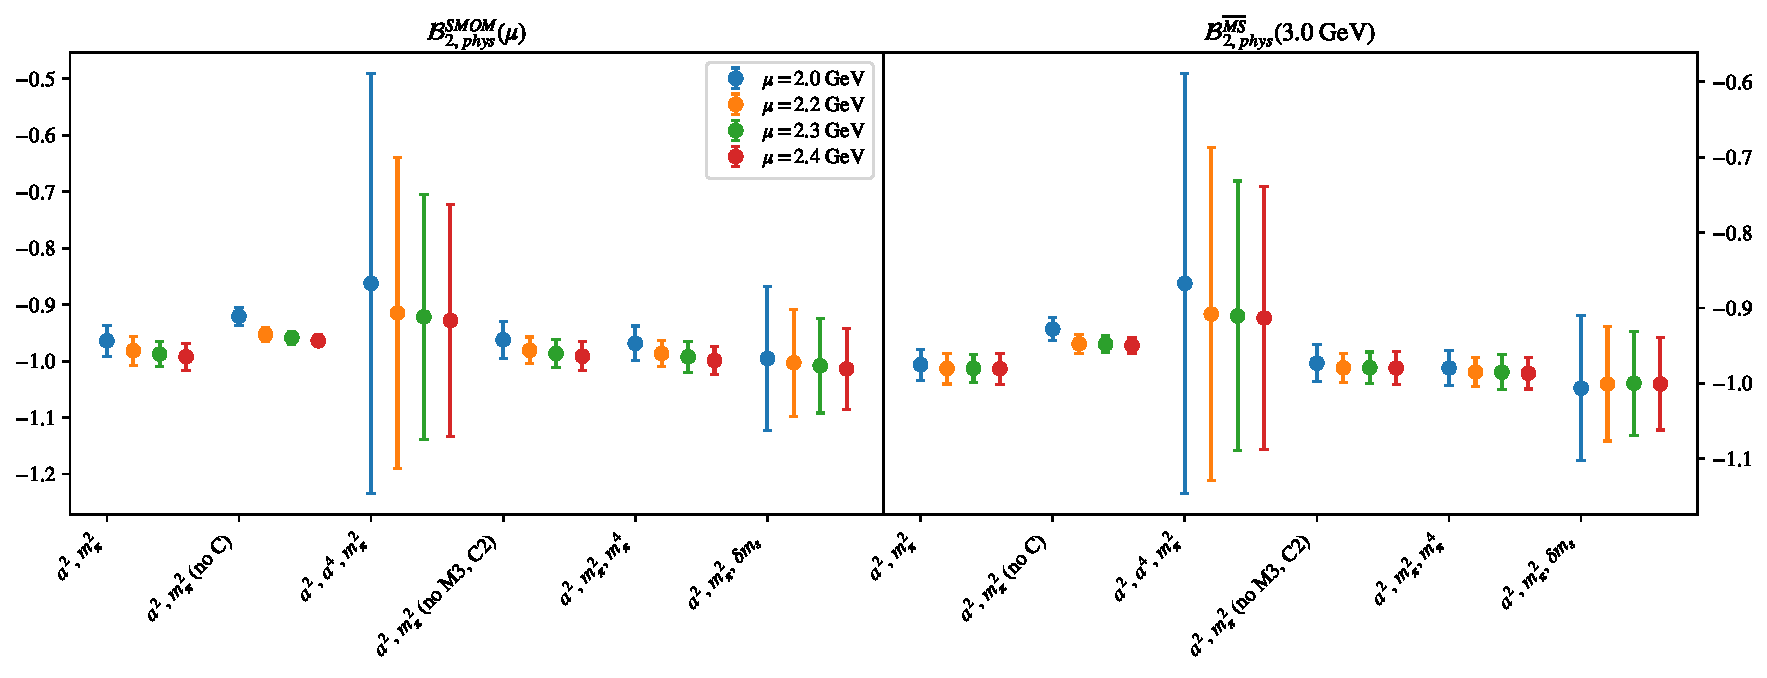
\includegraphics[page=1, width=1.1\textwidth]{VVmAA/NPR/fit_summary_bag.pdf}
\caption{$\mathcal{B}_{2}$\\(left) $\mathcal{B}_{phys}$ in RI/SMOM scheme from fit variations (fits with $p$-value $<0.05$ marked with ``$\times$"). \\(right) $\mathcal{B}_{phys}$ in $\overline{MS}$ computed using $\mathcal{B}^{\overline{MS}} = R^{\overline{MS}\leftarrow SMOM}(3.0)\sigma_{npt}(3.0,\mu) \mathcal{B}^{SMOM}(\mu)$.}
\end{figure}
\clearpage
\begin{figure}
\centering
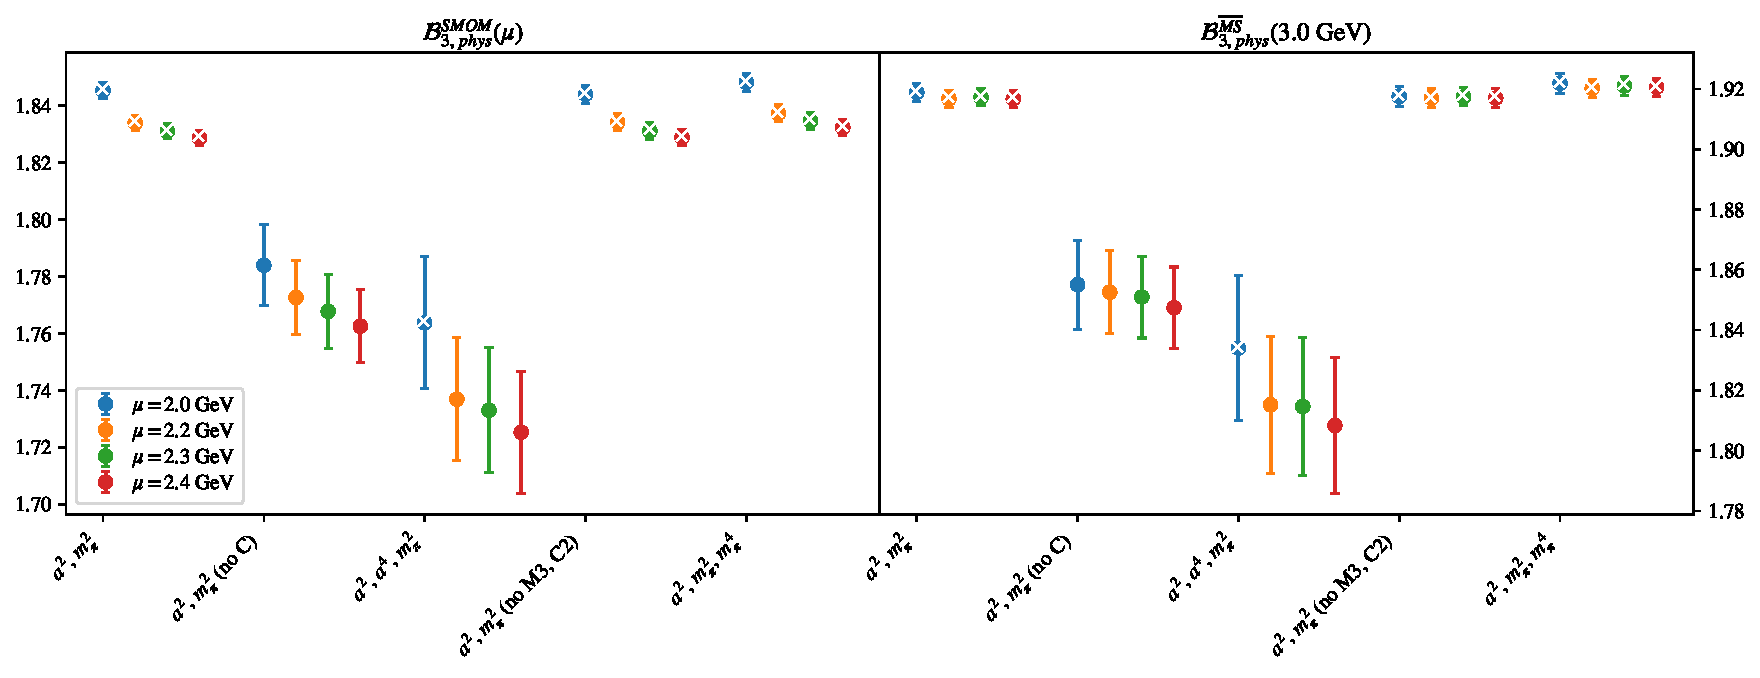
\includegraphics[page=1, width=1.1\textwidth]{SSmPP/NPR/fit_summary_bag.pdf}
\caption{$\mathcal{B}_{3}$\\(left) $\mathcal{B}_{phys}$ in RI/SMOM scheme from fit variations (fits with $p$-value $<0.05$ marked with ``$\times$"). \\(right) $\mathcal{B}_{phys}$ in $\overline{MS}$ computed using $\mathcal{B}^{\overline{MS}} = R^{\overline{MS}\leftarrow SMOM}(3.0)\sigma_{npt}(3.0,\mu) \mathcal{B}^{SMOM}(\mu)$.}
\end{figure}
\clearpage
\begin{figure}
\centering
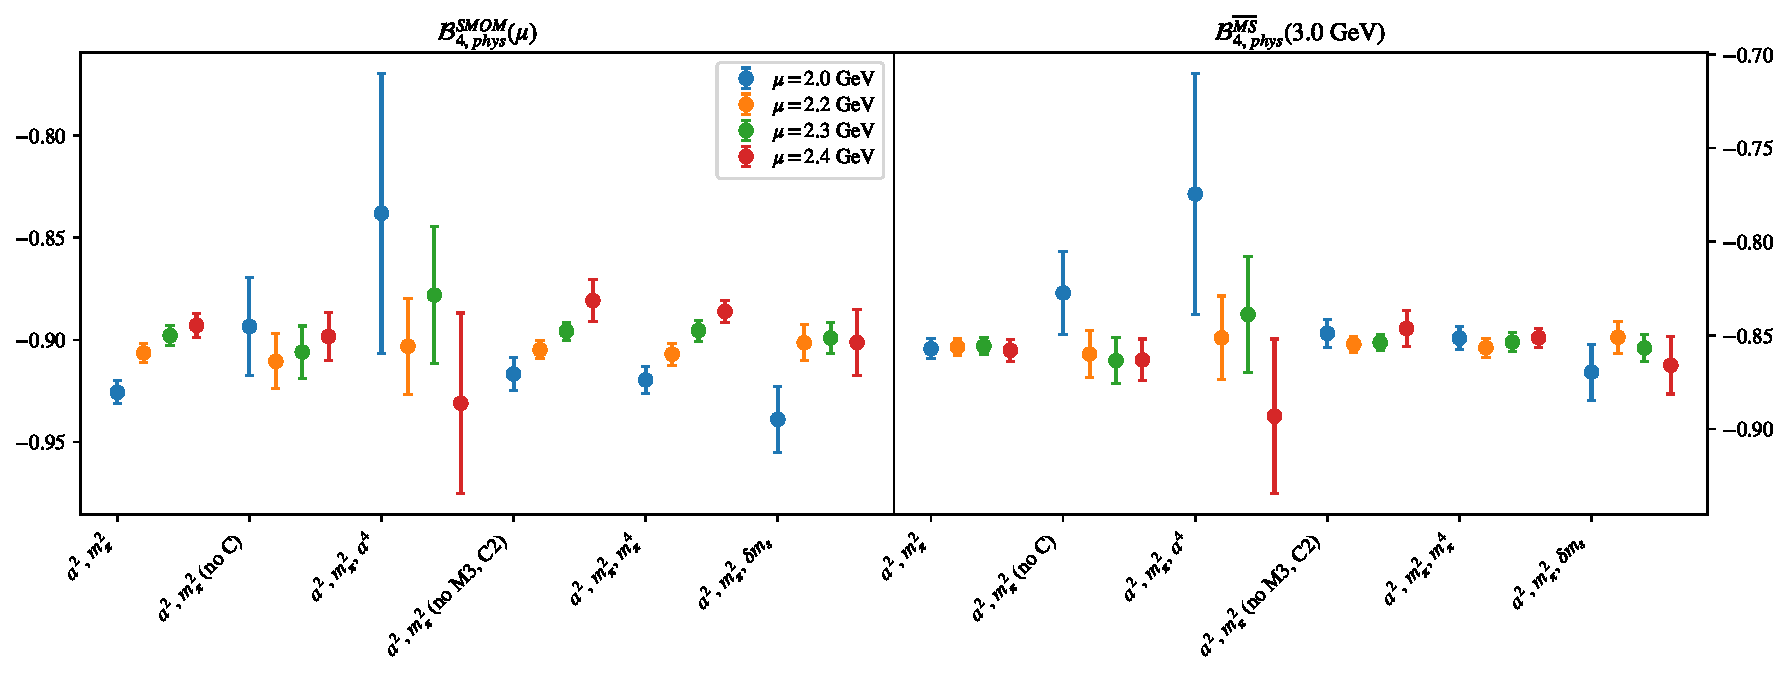
\includegraphics[page=1, width=1.1\textwidth]{SSpPP/NPR/fit_summary_bag.pdf}
\caption{$\mathcal{B}_{4}$\\(left) $\mathcal{B}_{phys}$ in RI/SMOM scheme from fit variations (fits with $p$-value $<0.05$ marked with ``$\times$"). \\(right) $\mathcal{B}_{phys}$ in $\overline{MS}$ computed using $\mathcal{B}^{\overline{MS}} = R^{\overline{MS}\leftarrow SMOM}(3.0)\sigma_{npt}(3.0,\mu) \mathcal{B}^{SMOM}(\mu)$.}
\end{figure}
\clearpage
\begin{figure}
\centering
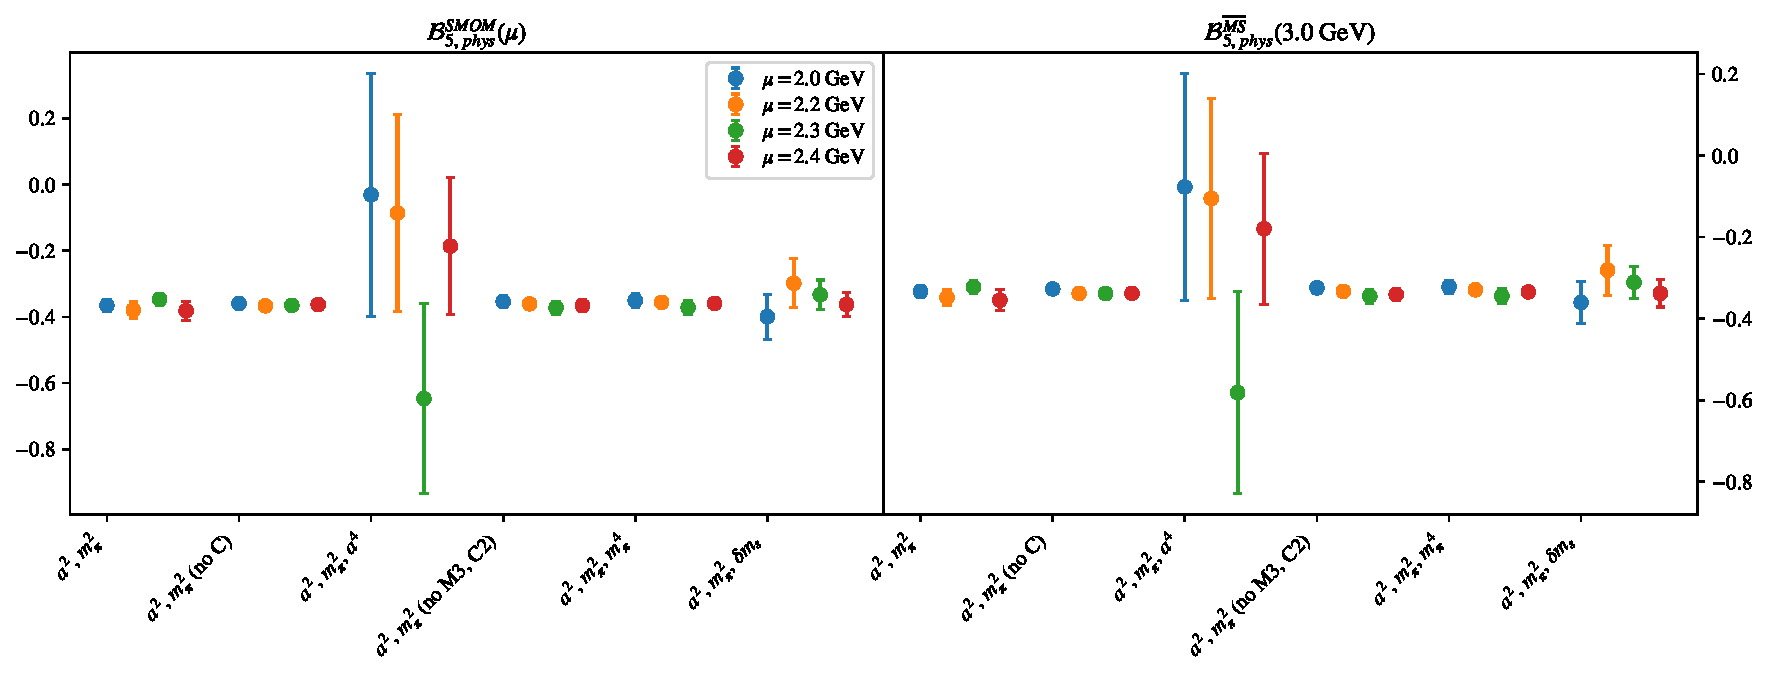
\includegraphics[page=1, width=1.1\textwidth]{TT/NPR/fit_summary_bag.pdf}
\caption{$\mathcal{B}_{5}$\\(left) $\mathcal{B}_{phys}$ in RI/SMOM scheme from fit variations (fits with $p$-value $<0.05$ marked with ``$\times$"). \\(right) $\mathcal{B}_{phys}$ in $\overline{MS}$ computed using $\mathcal{B}^{\overline{MS}} = R^{\overline{MS}\leftarrow SMOM}(3.0)\sigma_{npt}(3.0,\mu) \mathcal{B}^{SMOM}(\mu)$.}
\end{figure}
\clearpage
\section{$\mathcal{B}_1$}
\begin{table}[h!]
\begin{center}
\begin{tabular}{|c|c|c|c|c|c|c|}
\hline
$\mu$ (GeV) & $a^2$, $m_\pi^2$& $a^2$, $m_\pi^2$ (no C)& $a^2$, $m_\pi^2$, $a^4$& $a^2$, $m_\pi^2$ (no M3, C2)& $a^2$, $m_\pi^2$, $m_\pi^4$& $a^2$, $m_\pi^2$, $\delta m_s$\\
\hline
2.0& \hyperlink{VVpAA/NPR/bag_a2m2_20.pdf.1}{\textbf{1.4039(27)}: 1.874 (0.095)} & \hyperlink{VVpAA/NPR/bag_a2m2noC_20.pdf.1}{\textbf{1.416(12)}: 0.916 (0.4)} & \hyperlink{VVpAA/NPR/bag_a2a4m2_20.pdf.1}{\textbf{1.421(21)}: 2.17 (0.07)} & \hyperlink{VVpAA/NPR/bag_a2m2mcut_20.pdf.1}{\textbf{1.4090(32)}: 0.266 (0.85)} & \hyperlink{VVpAA/NPR/bag_a2m2m4_20.pdf.1}{\textbf{1.4092(33)}: 0.7 (0.592)} & \hyperlink{VVpAA/NPR/bag_a2m2delm_20.pdf.1}{\textbf{1.4018(31)}: 1.883 (0.11)}\\
2.2& \hyperlink{VVpAA/NPR/bag_a2m2_22.pdf.1}{\textbf{1.3963(27)}: 2.212 (0.05)} & \hyperlink{VVpAA/NPR/bag_a2m2noC_22.pdf.1}{\textbf{1.411(12)}: 1.164 (0.312)} & \hyperlink{VVpAA/NPR/bag_a2a4m2_22.pdf.1}{\textbf{1.417(21)}: 2.52 (0.039)} & \hyperlink{VVpAA/NPR/bag_a2m2mcut_22.pdf.1}{\textbf{1.4018(32)}: 0.363 (0.78)} & \hyperlink{VVpAA/NPR/bag_a2m2m4_22.pdf.1}{\textbf{1.4020(33)}: 0.923 (0.449)} & \hyperlink{VVpAA/NPR/bag_a2m2delm_22.pdf.1}{\textbf{1.3940(31)}: 2.145 (0.073)}\\
2.3& \hyperlink{VVpAA/NPR/bag_a2m2_23.pdf.1}{\textbf{1.3931(27)}: 2.29 (0.043)} & \hyperlink{VVpAA/NPR/bag_a2m2noC_23.pdf.1}{\textbf{1.408(12)}: 1.203 (0.3)} & \hyperlink{VVpAA/NPR/bag_a2a4m2_23.pdf.1}{\textbf{1.415(20)}: 2.592 (0.035)} & \hyperlink{VVpAA/NPR/bag_a2m2mcut_23.pdf.1}{\textbf{1.3986(32)}: 0.406 (0.749)} & \hyperlink{VVpAA/NPR/bag_a2m2m4_23.pdf.1}{\textbf{1.3988(33)}: 0.978 (0.418)} & \hyperlink{VVpAA/NPR/bag_a2m2delm_23.pdf.1}{\textbf{1.3906(31)}: 2.186 (0.068)}\\
2.4& \hyperlink{VVpAA/NPR/bag_a2m2_24.pdf.1}{\textbf{1.3902(27)}: 2.351 (0.038)} & \hyperlink{VVpAA/NPR/bag_a2m2noC_24.pdf.1}{\textbf{1.406(12)}: 1.243 (0.288)} & \hyperlink{VVpAA/NPR/bag_a2a4m2_24.pdf.1}{\textbf{1.412(20)}: 2.662 (0.031)} & \hyperlink{VVpAA/NPR/bag_a2m2mcut_24.pdf.1}{\textbf{1.3958(32)}: 0.416 (0.742)} & \hyperlink{VVpAA/NPR/bag_a2m2m4_24.pdf.1}{\textbf{1.3960(33)}: 1.007 (0.402)} & \hyperlink{VVpAA/NPR/bag_a2m2delm_24.pdf.1}{\textbf{1.3877(31)}: 2.239 (0.062)}\\
\hline
\end{tabular}
\caption{Physical point value from chiral and continuum extrapolation at renormalisation scale $\mu$. Entries are \textbf{value(error)}: $\chi^2/\text{DOF}$ ($p$-value).}
\end{center}
\end{table}
\begin{table}[h!]
\begin{center}
\begin{tabular}{|c c|c|c|c|c|c|c|}
\hline
$\mu$ (GeV) &  & $a^2$, $m_\pi^2$& $a^2$, $m_\pi^2$ (no C)& $a^2$, $m_\pi^2$, $a^4$& $a^2$, $m_\pi^2$ (no M3, C2)& $a^2$, $m_\pi^2$, $m_\pi^4$& $a^2$, $m_\pi^2$, $\delta m_s$\\
\hline
\multirow{3}{0.5in}{2.0} & $\alpha$ & 0.1314(97)& 0.067(75)& -0.03(19)& 0.115(11)& 0.114(11)& 0.138(11)\\
 & $\beta$ & 0.00367(20)& 0.00318(38)& 0.00375(22)& 0.00266(40)& 0.0005(12)& 0.00380(22)\\
 & $\gamma$ &  &  & 0.33(40)&  & 0.00028(10)& -0.0044(33)\\
\hline
\multirow{3}{0.5in}{2.2} & $\alpha$ & 0.1368(97)& 0.059(74)& -0.06(19)& 0.119(11)& 0.119(11)& 0.145(10)\\
 & $\beta$ & 0.00365(20)& 0.00312(38)& 0.00375(22)& 0.00258(40)& 0.0003(12)& 0.00381(22)\\
 & $\gamma$ &  &  & 0.39(39)&  & 0.00030(10)& -0.0050(32)\\
\hline
\multirow{3}{0.5in}{2.3} & $\alpha$ & 0.1385(96)& 0.057(74)& -0.06(19)& 0.120(11)& 0.120(11)& 0.147(10)\\
 & $\beta$ & 0.00366(20)& 0.00311(38)& 0.00376(22)& 0.00257(39)& 0.0003(12)& 0.00382(22)\\
 & $\gamma$ &  &  & 0.41(39)&  & 0.00030(10)& -0.0052(32)\\
\hline
\multirow{3}{0.5in}{2.4} & $\alpha$ & 0.1393(96)& 0.056(74)& -0.06(19)& 0.121(11)& 0.121(11)& 0.147(10)\\
 & $\beta$ & 0.00366(20)& 0.00311(38)& 0.00377(22)& 0.00257(39)& 0.0002(12)& 0.00383(22)\\
 & $\gamma$ &  &  & 0.41(39)&  & 0.00030(10)& -0.0053(32)\\
\hline
\end{tabular}
\caption{Fit values of coefficients in $Q = Q_{phys} + \mathbf{\alpha} a^2 + \mathbf{\beta}\left(\frac{m_\pi^2}{f_\pi^2}-\frac{m_{\pi,PDG}^2}{f_\pi^2}\right) + \gamma(\ldots)$}
\end{center}
\end{table}
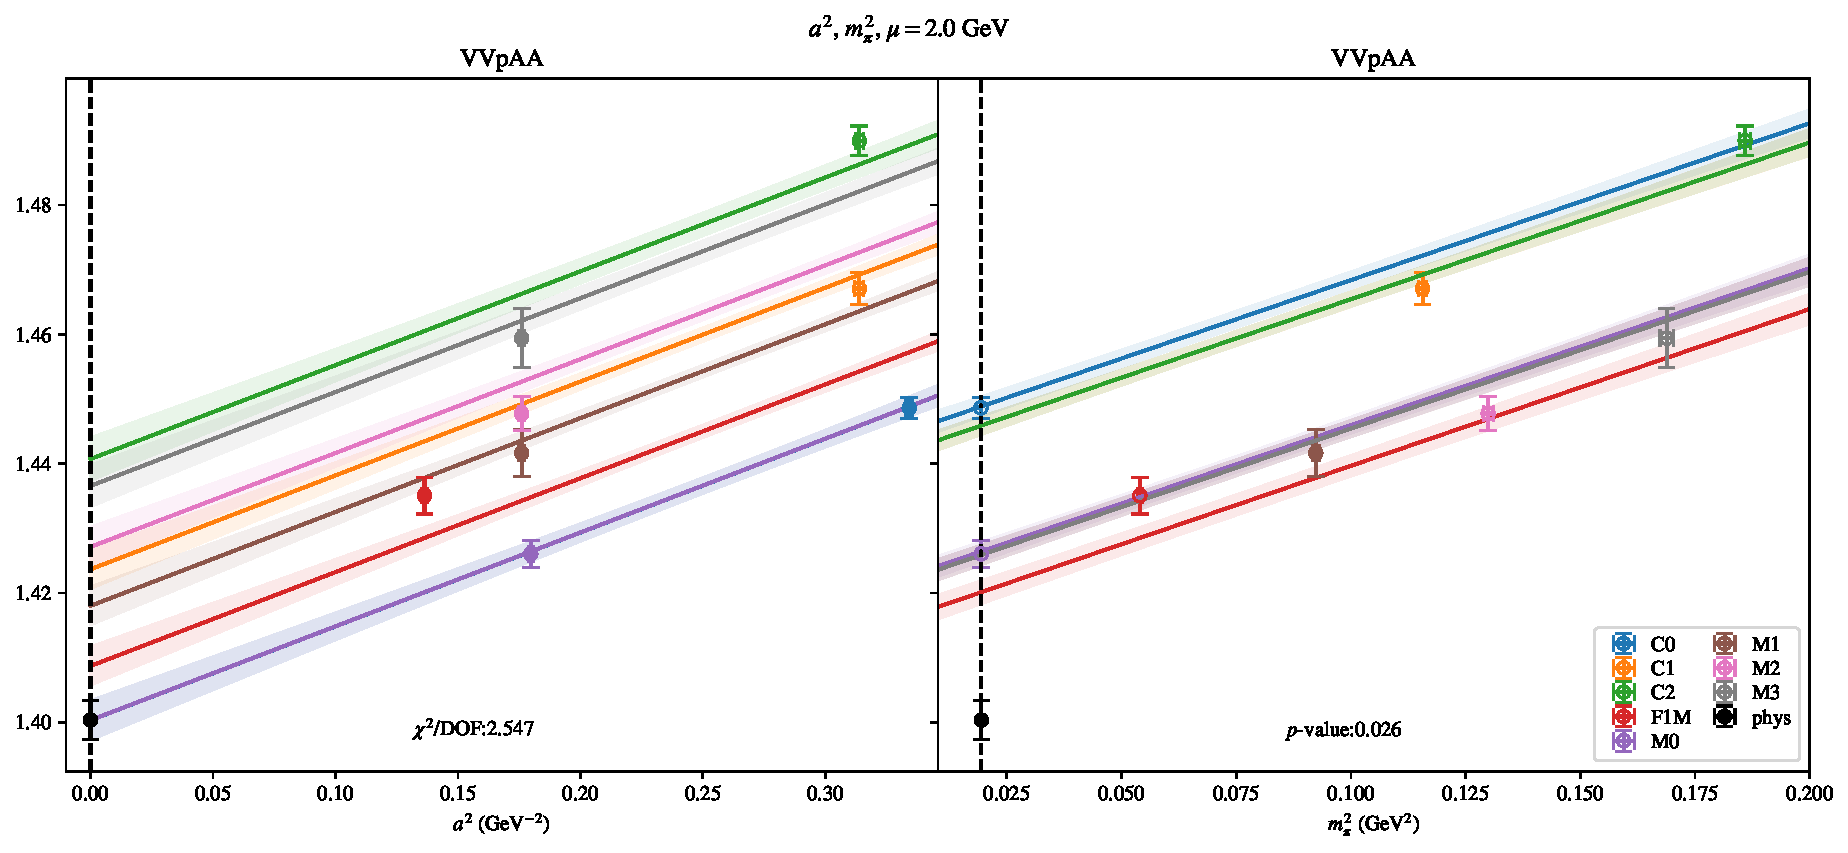
\includepdf[link, pages=-]{VVpAA/NPR/bag_a2m2_20.pdf}
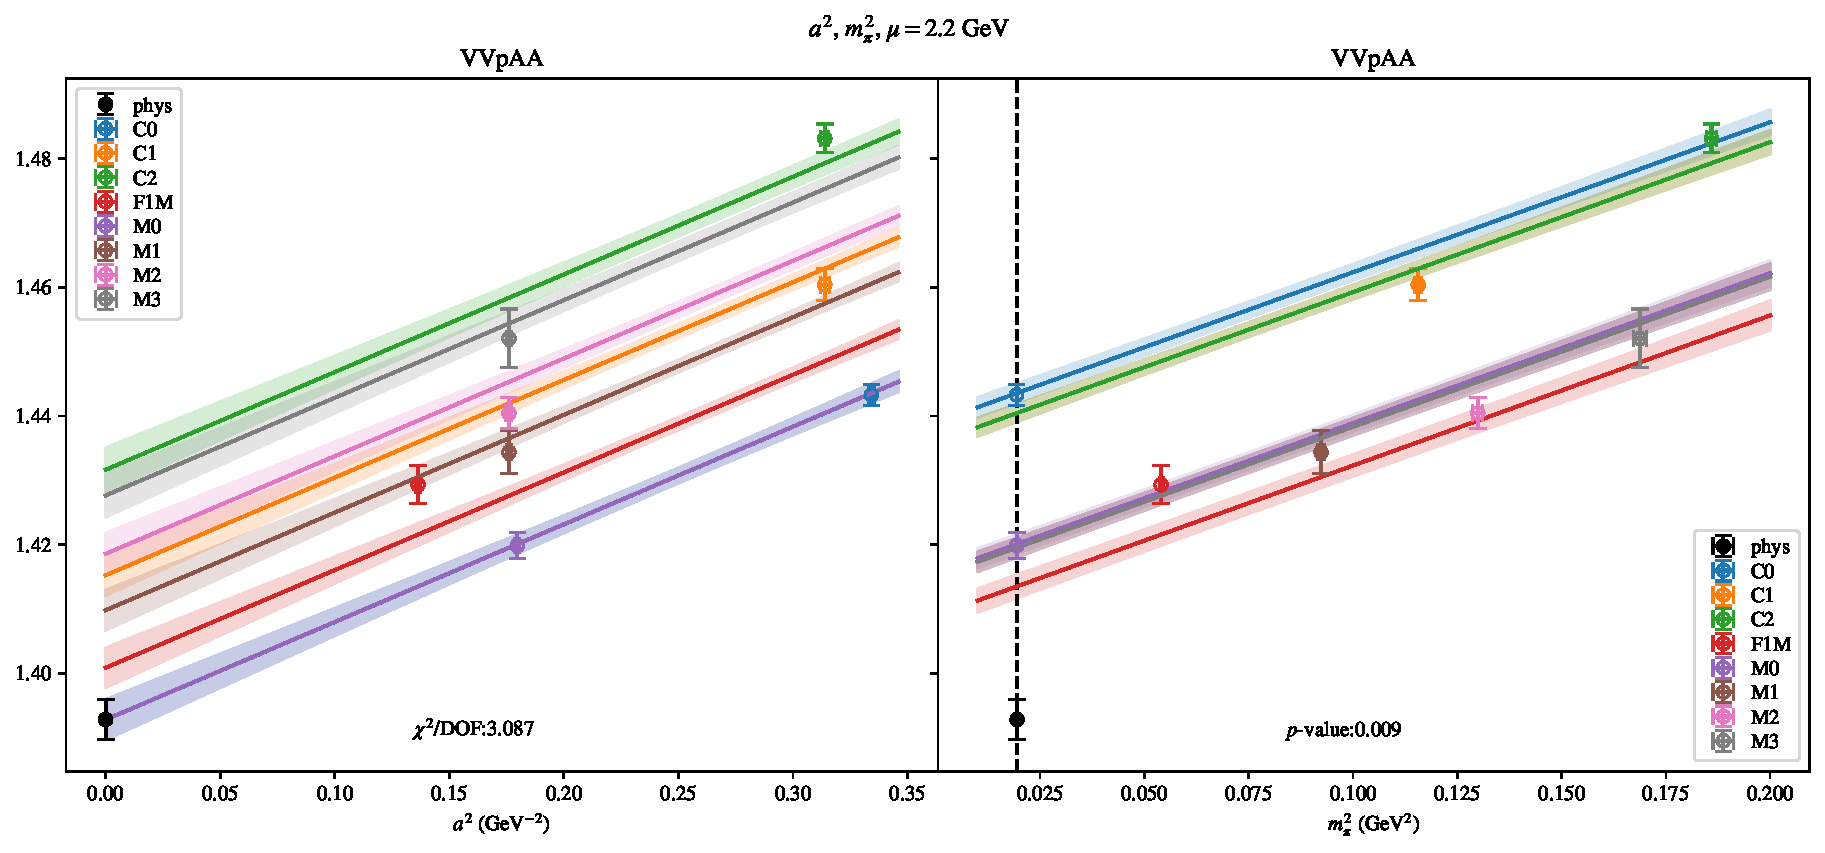
\includepdf[link, pages=-]{VVpAA/NPR/bag_a2m2_22.pdf}
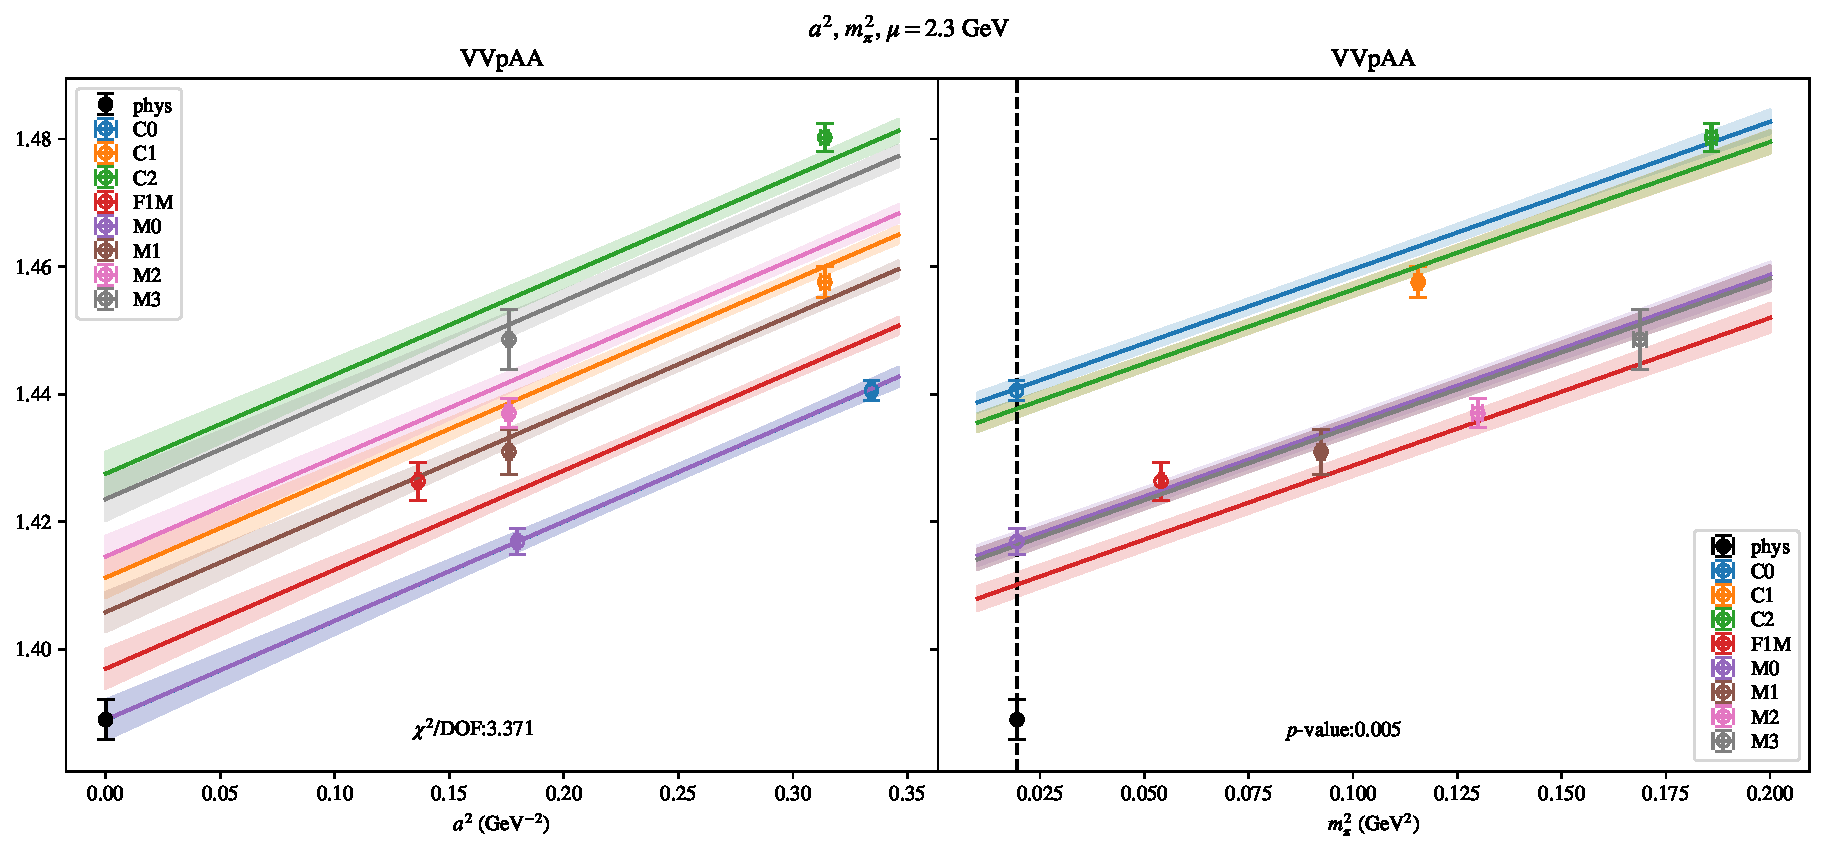
\includepdf[link, pages=-]{VVpAA/NPR/bag_a2m2_23.pdf}
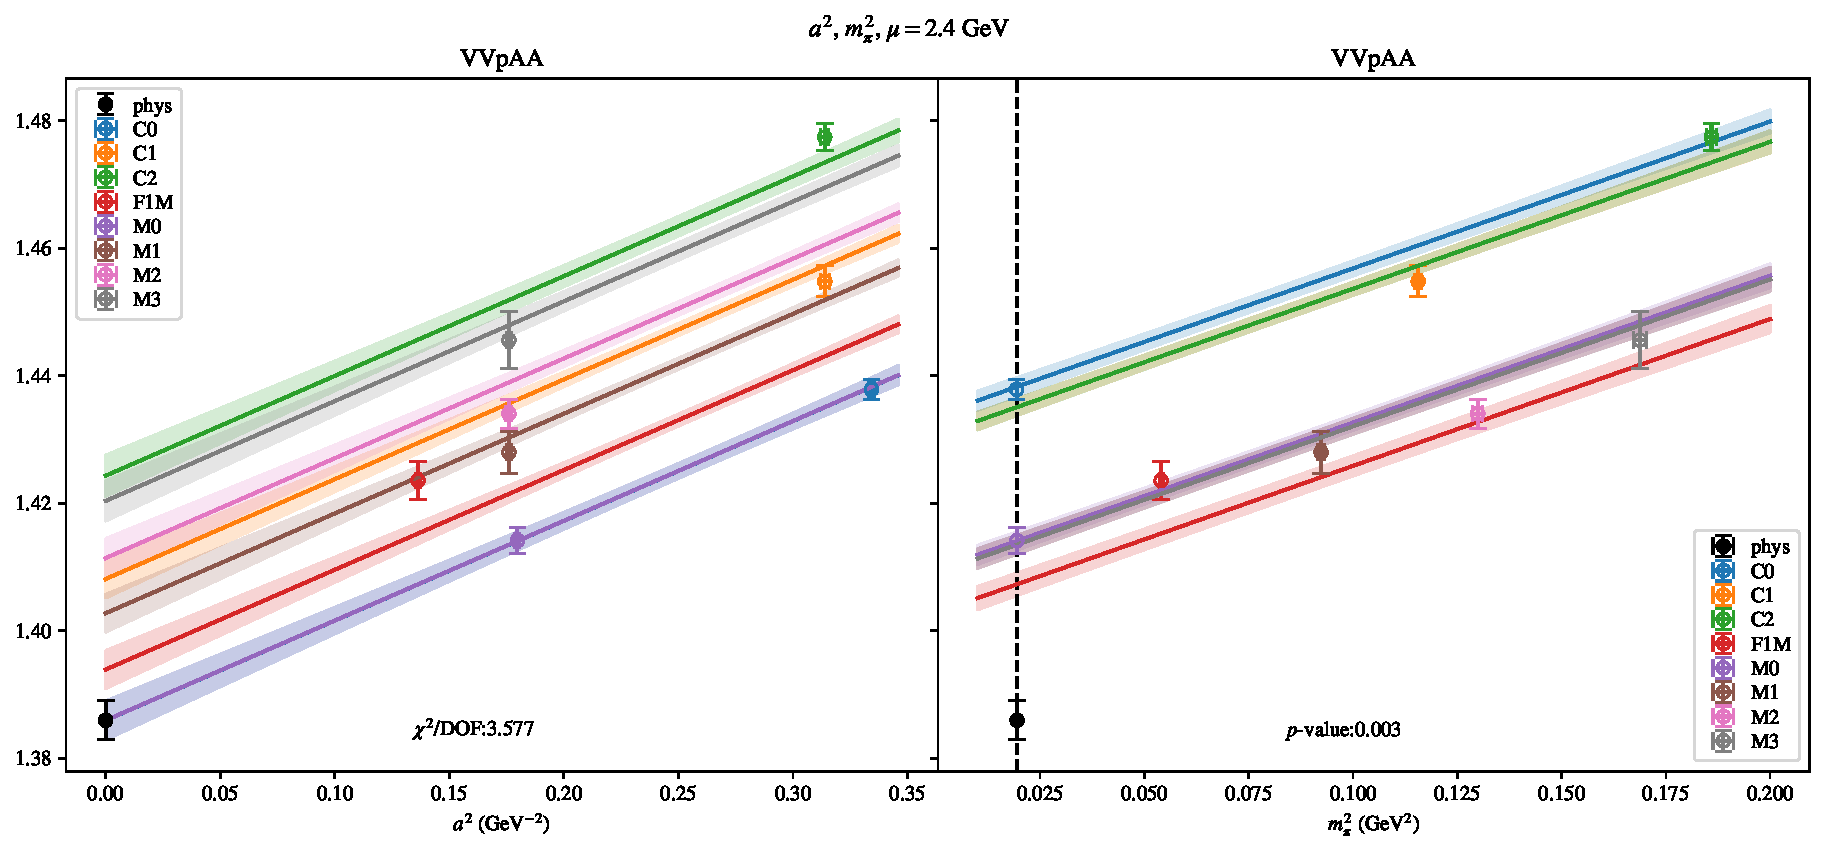
\includepdf[link, pages=-]{VVpAA/NPR/bag_a2m2_24.pdf}
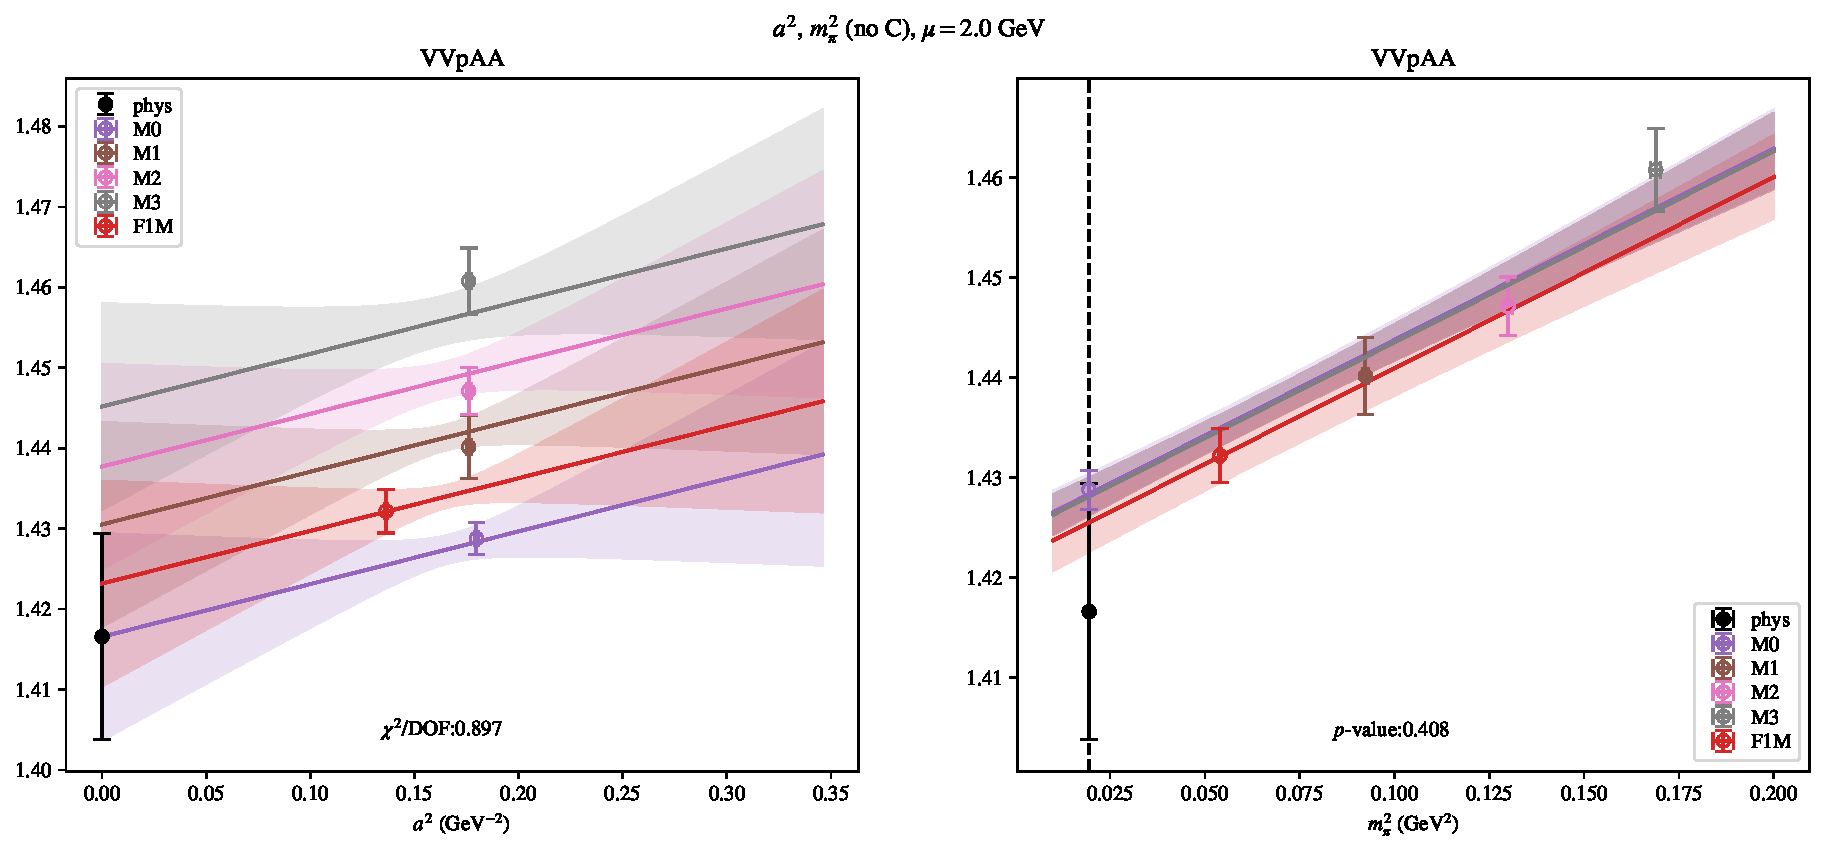
\includepdf[link, pages=-]{VVpAA/NPR/bag_a2m2noC_20.pdf}
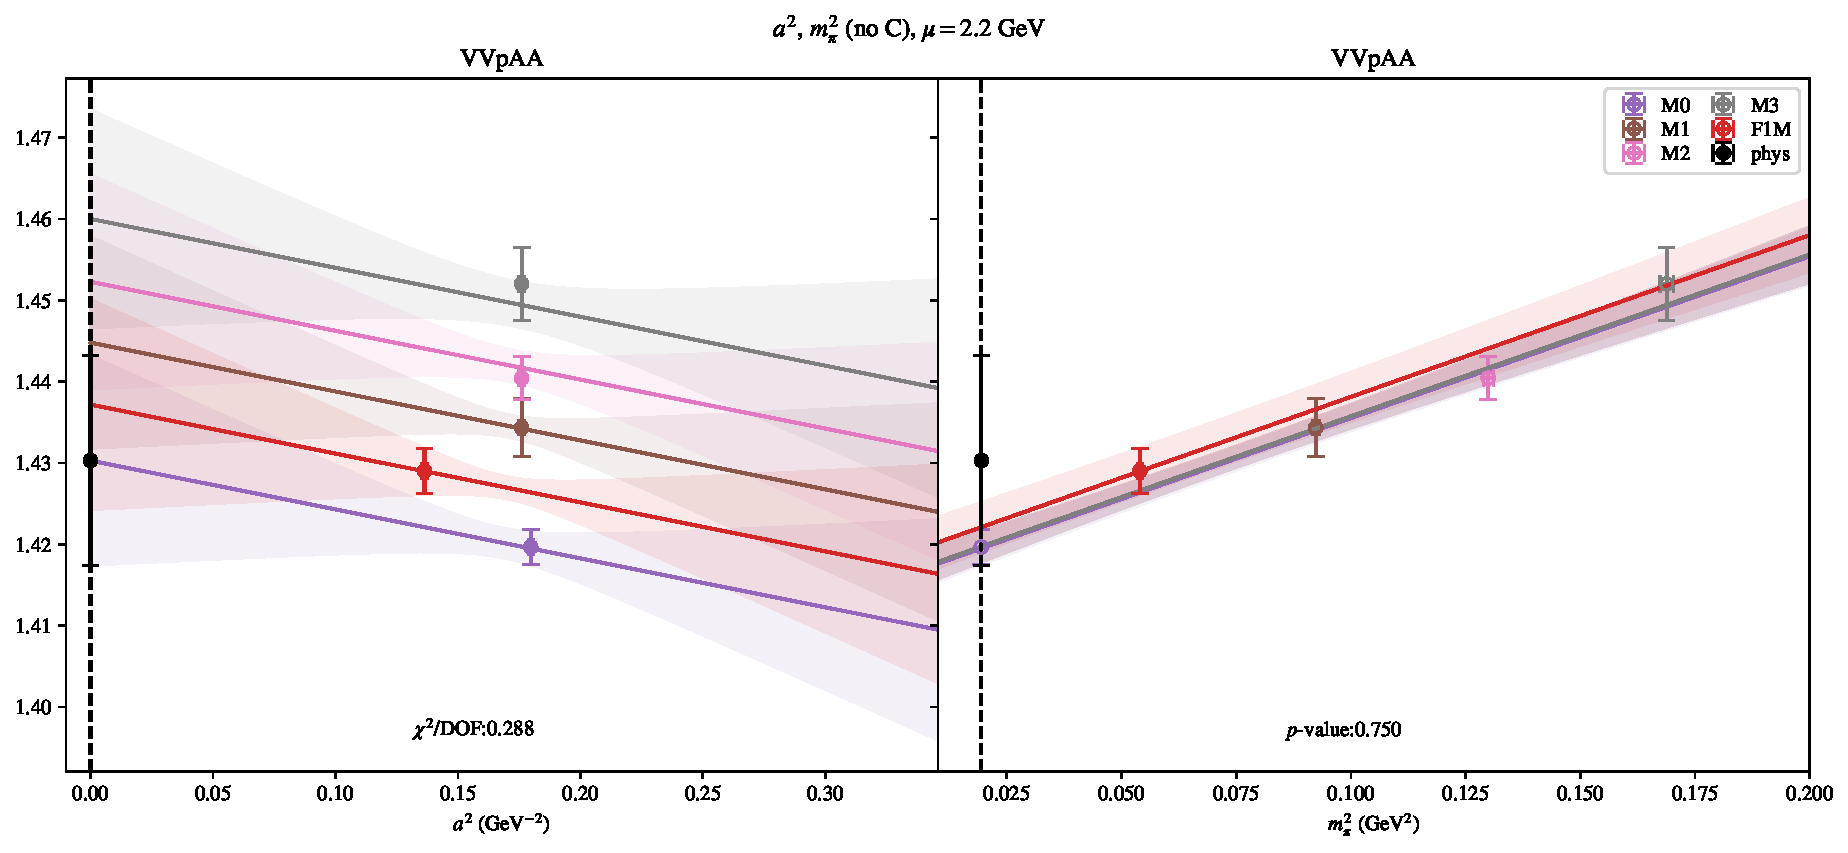
\includepdf[link, pages=-]{VVpAA/NPR/bag_a2m2noC_22.pdf}
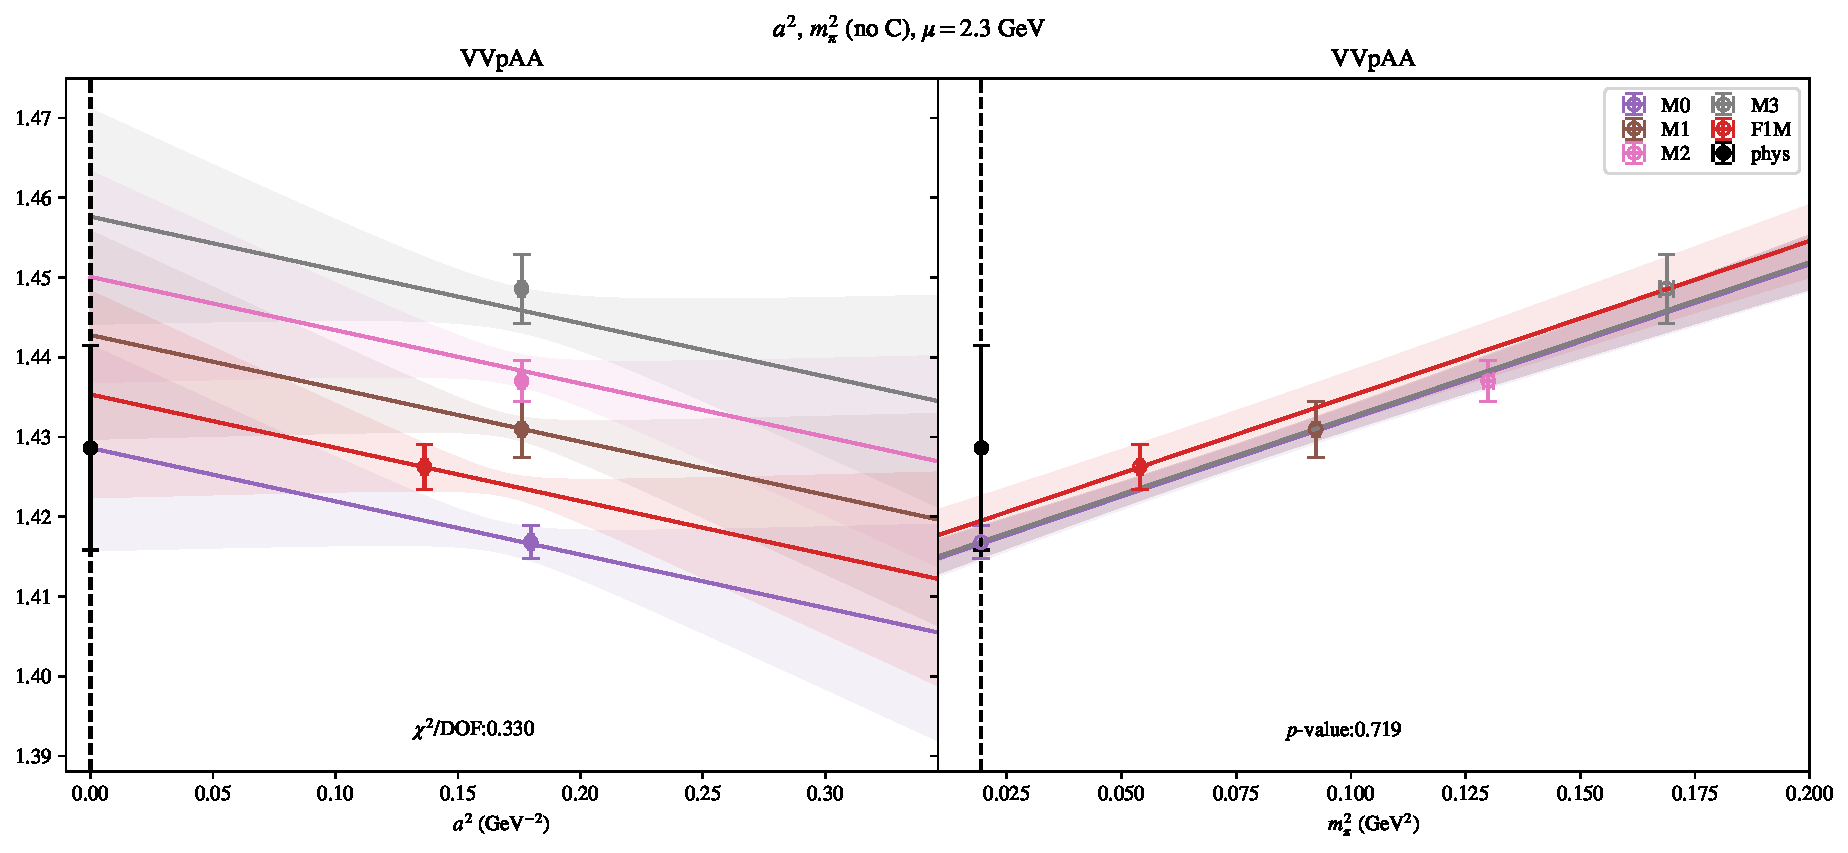
\includepdf[link, pages=-]{VVpAA/NPR/bag_a2m2noC_23.pdf}
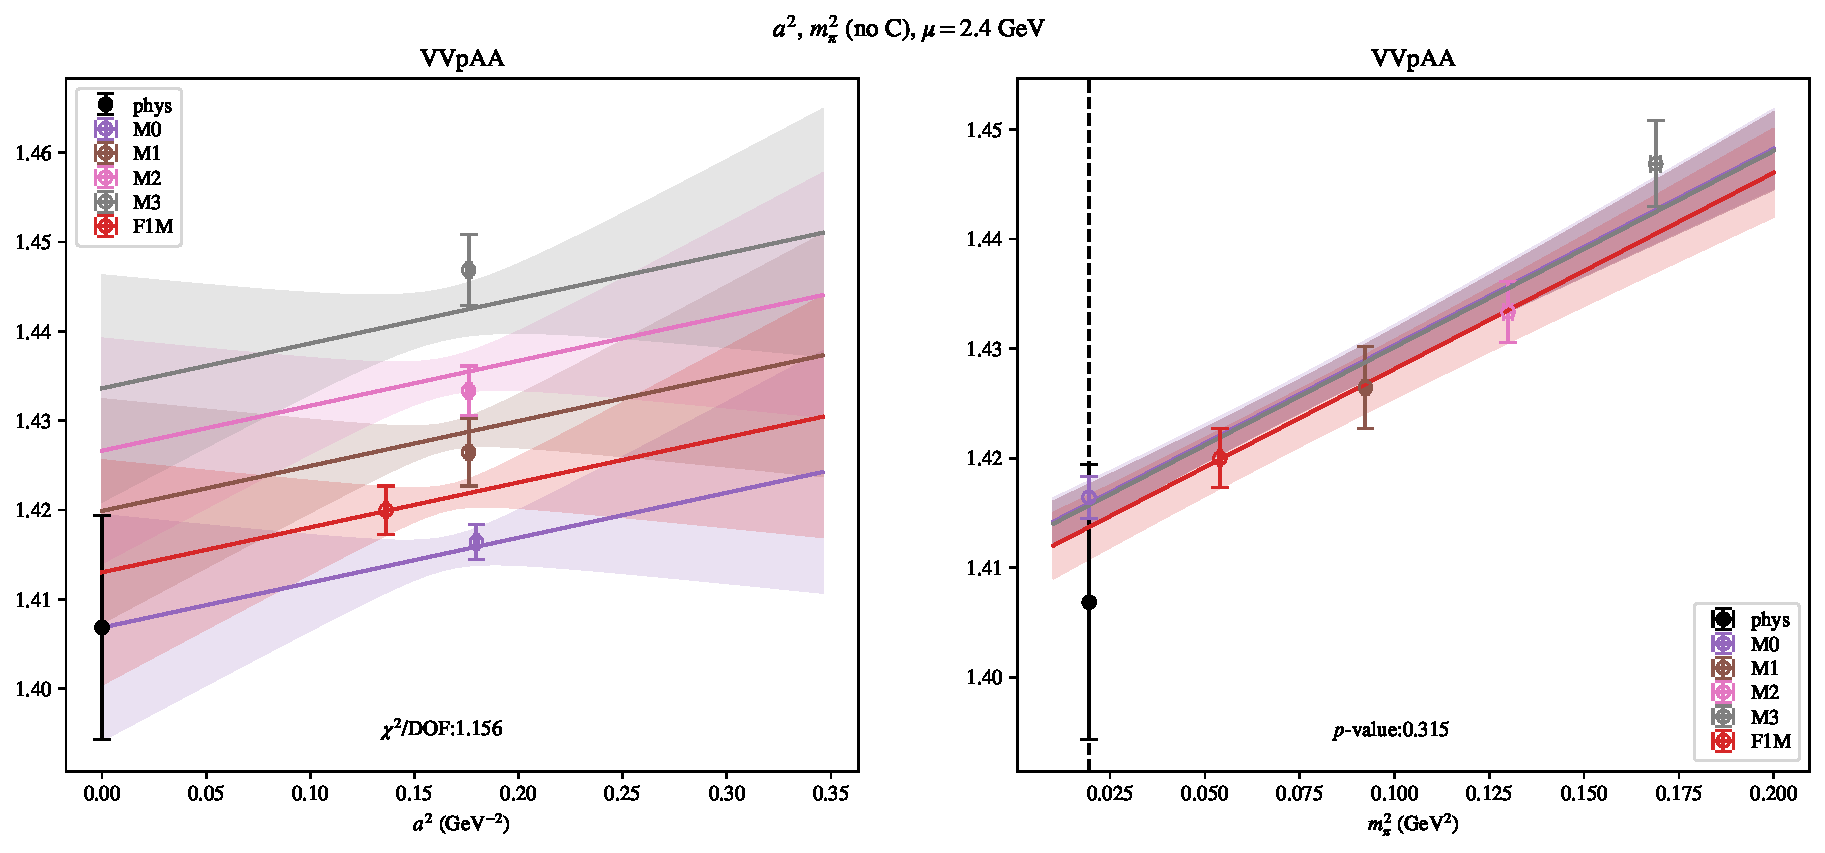
\includepdf[link, pages=-]{VVpAA/NPR/bag_a2m2noC_24.pdf}
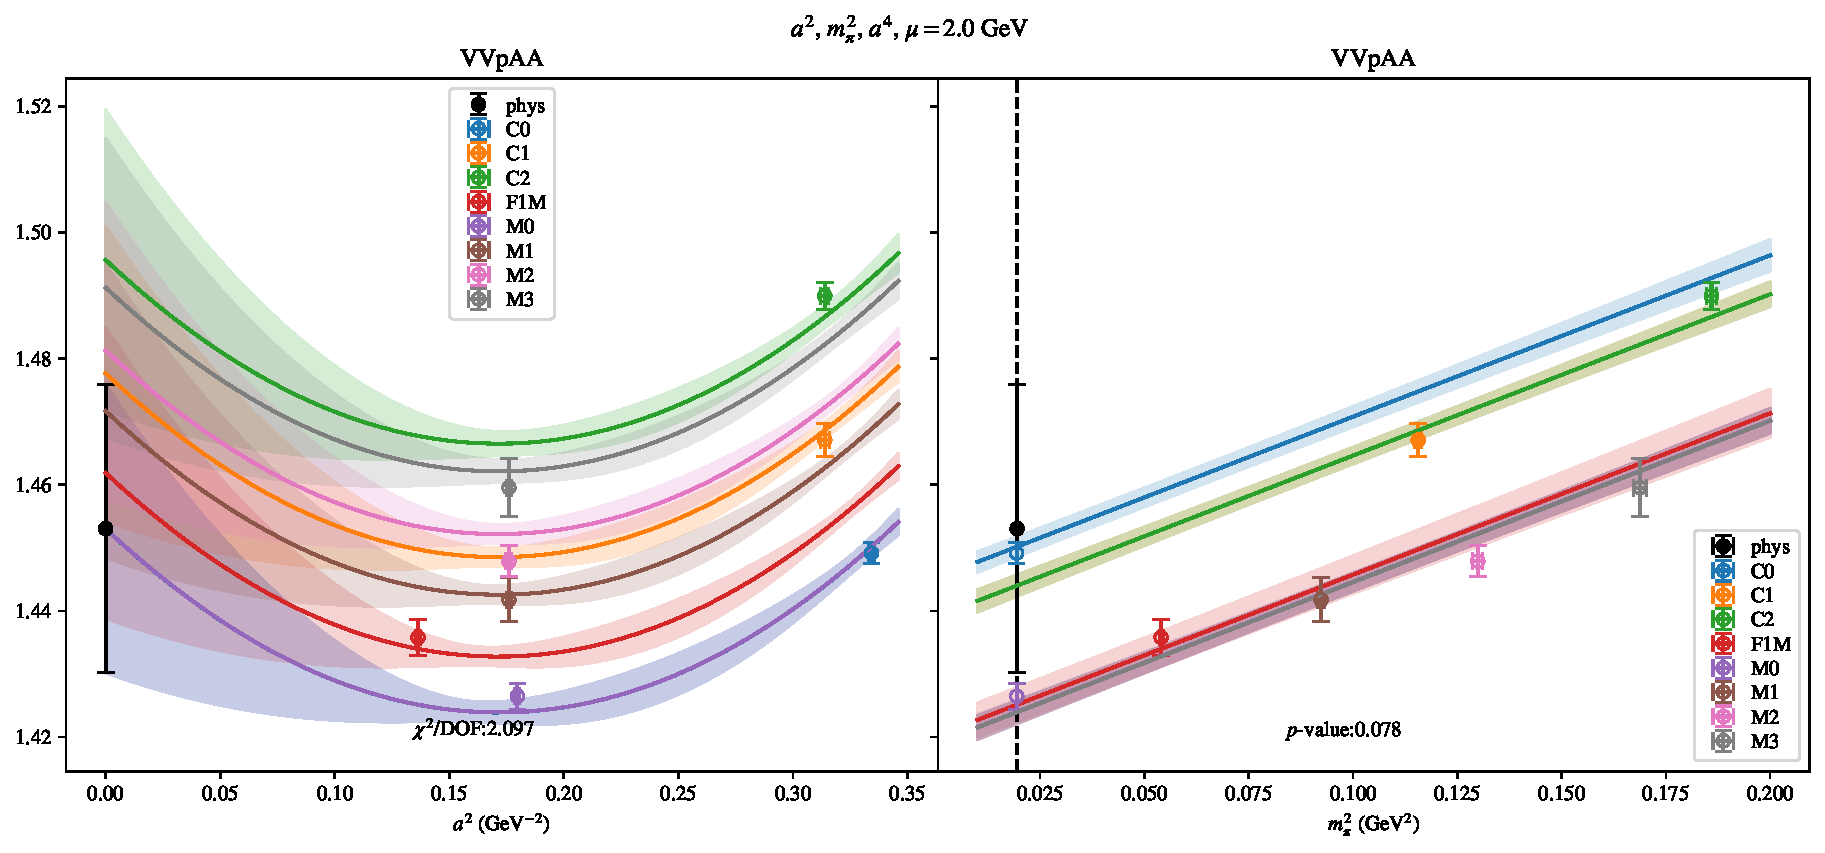
\includepdf[link, pages=-]{VVpAA/NPR/bag_a2a4m2_20.pdf}
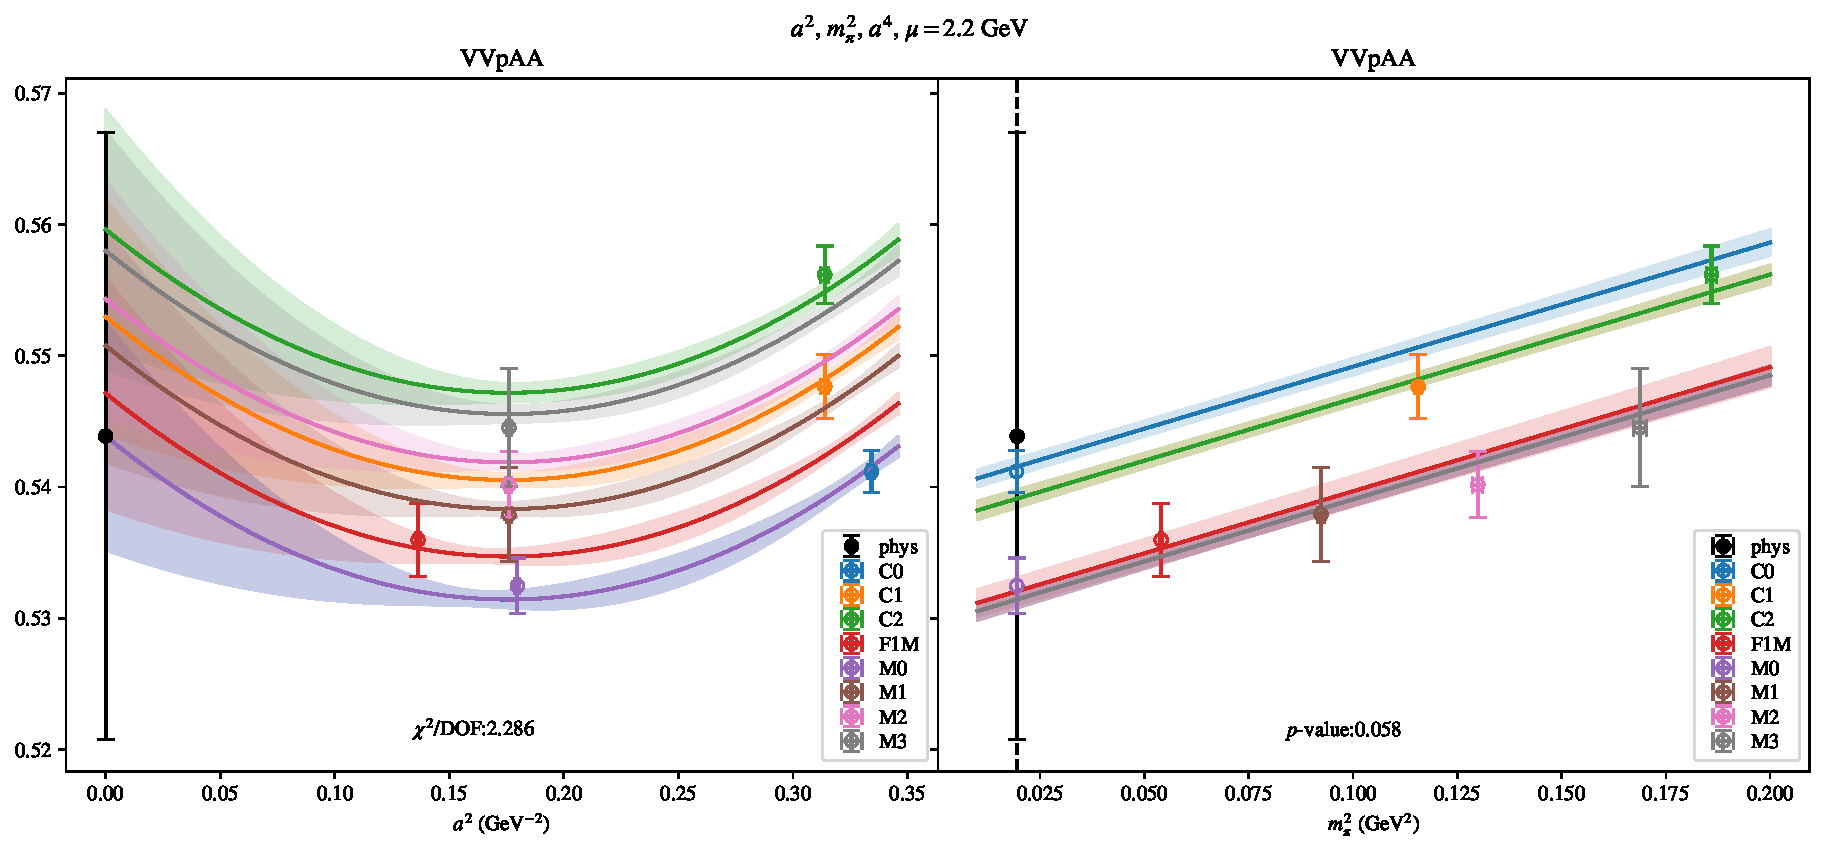
\includepdf[link, pages=-]{VVpAA/NPR/bag_a2a4m2_22.pdf}
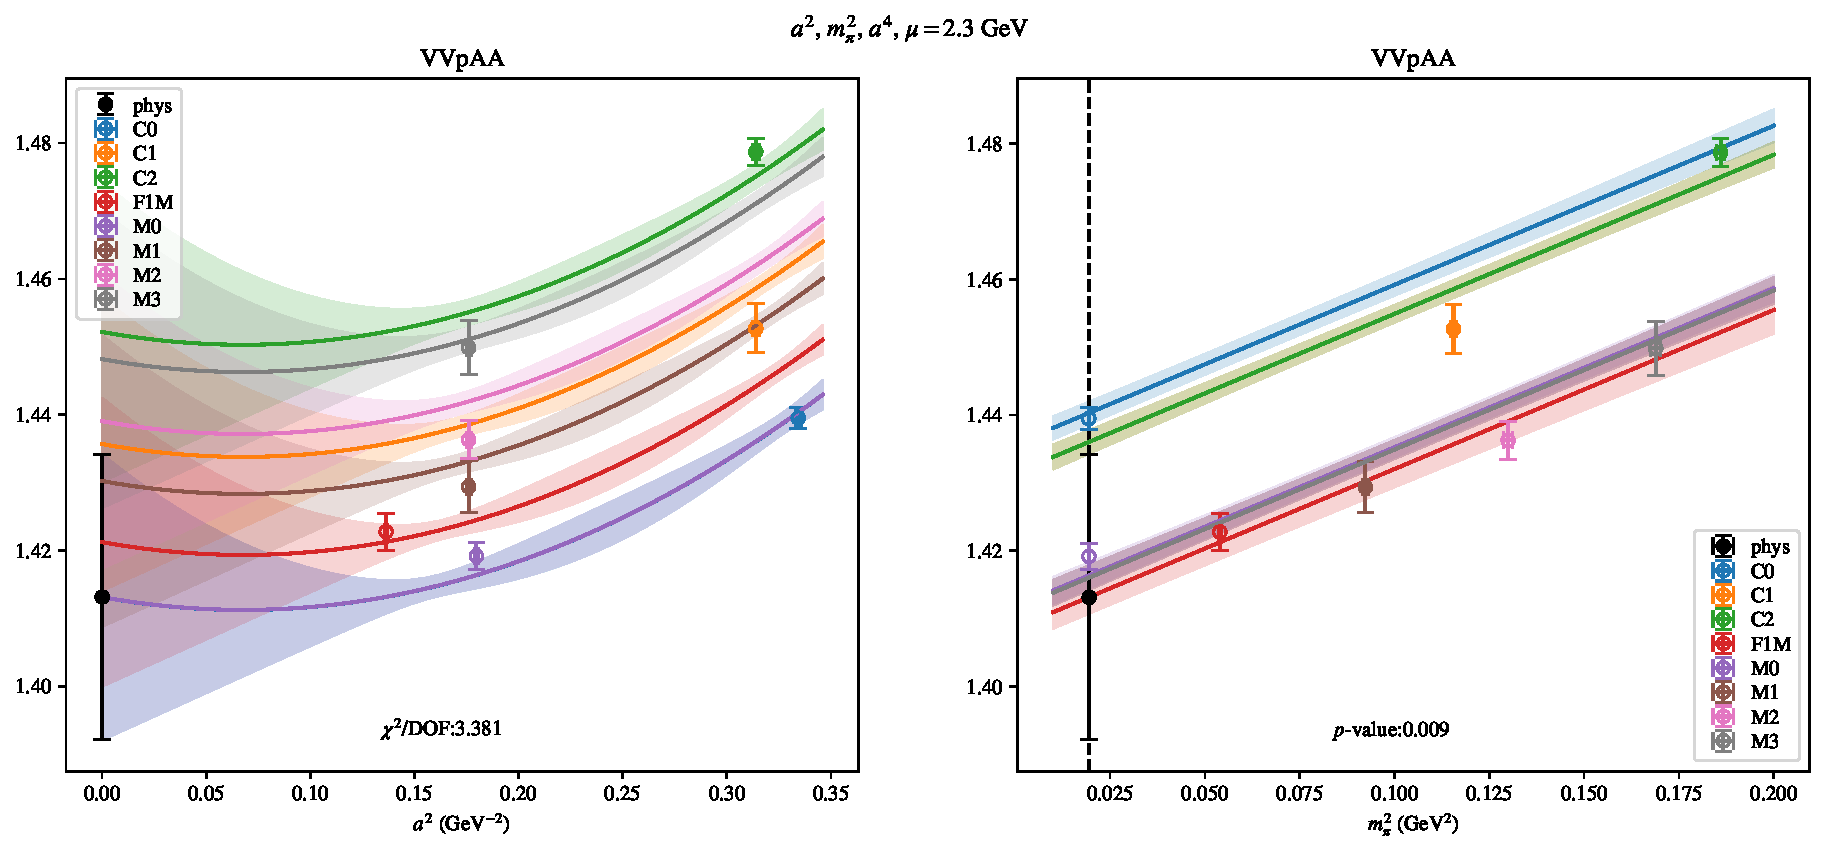
\includepdf[link, pages=-]{VVpAA/NPR/bag_a2a4m2_23.pdf}
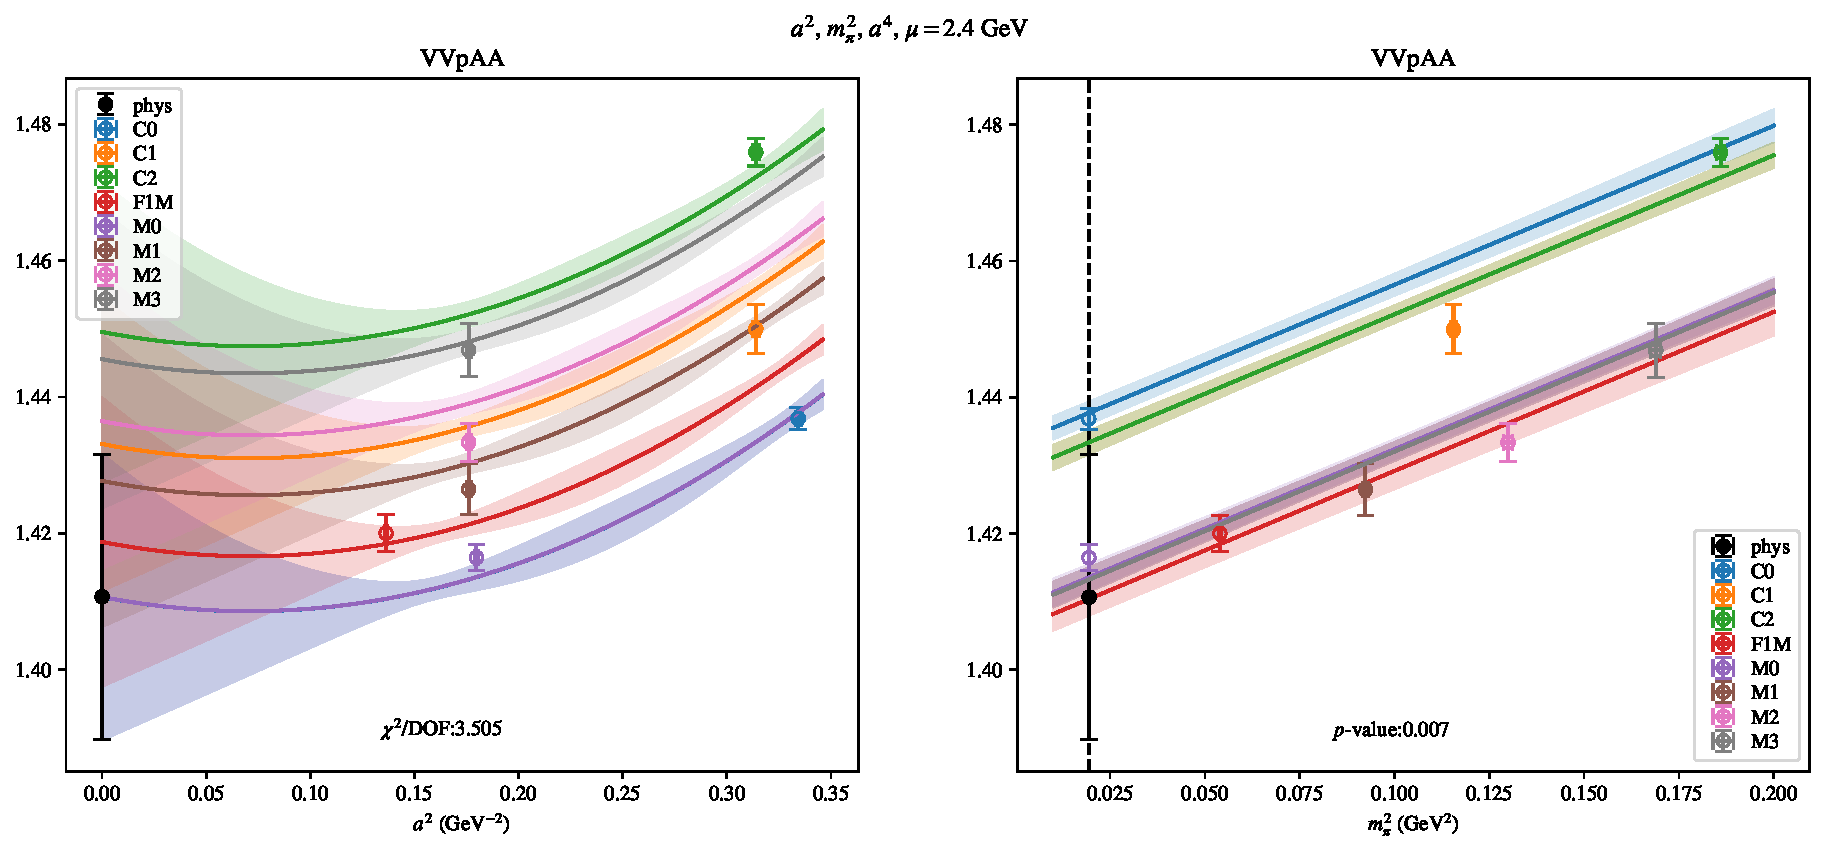
\includepdf[link, pages=-]{VVpAA/NPR/bag_a2a4m2_24.pdf}
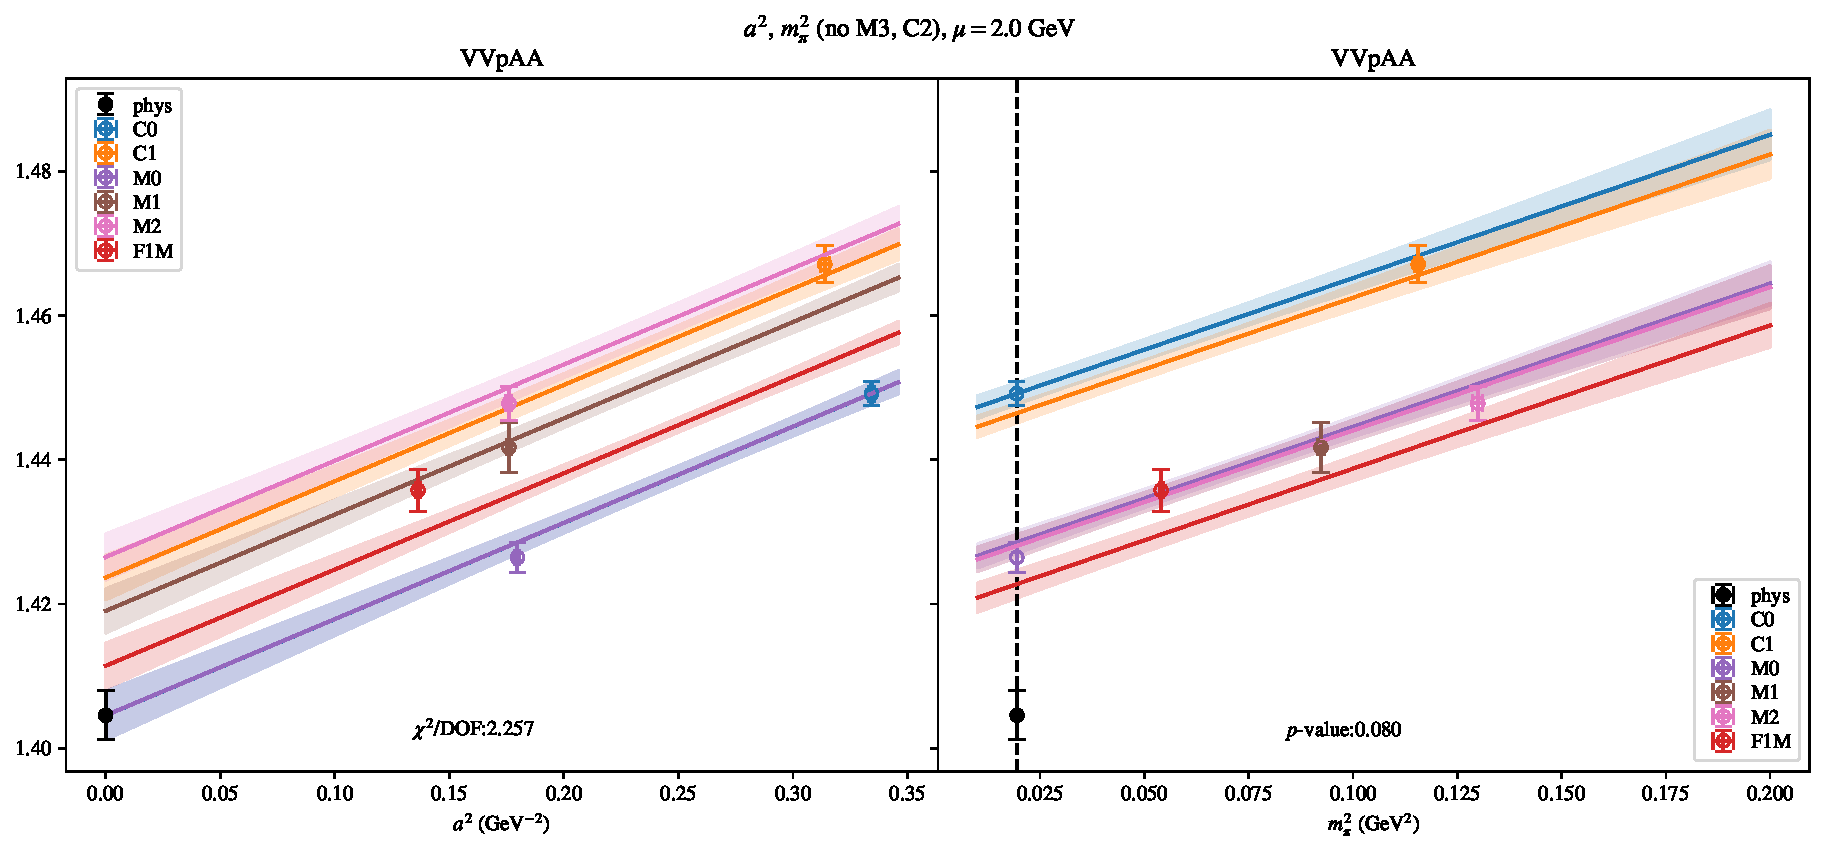
\includepdf[link, pages=-]{VVpAA/NPR/bag_a2m2mcut_20.pdf}
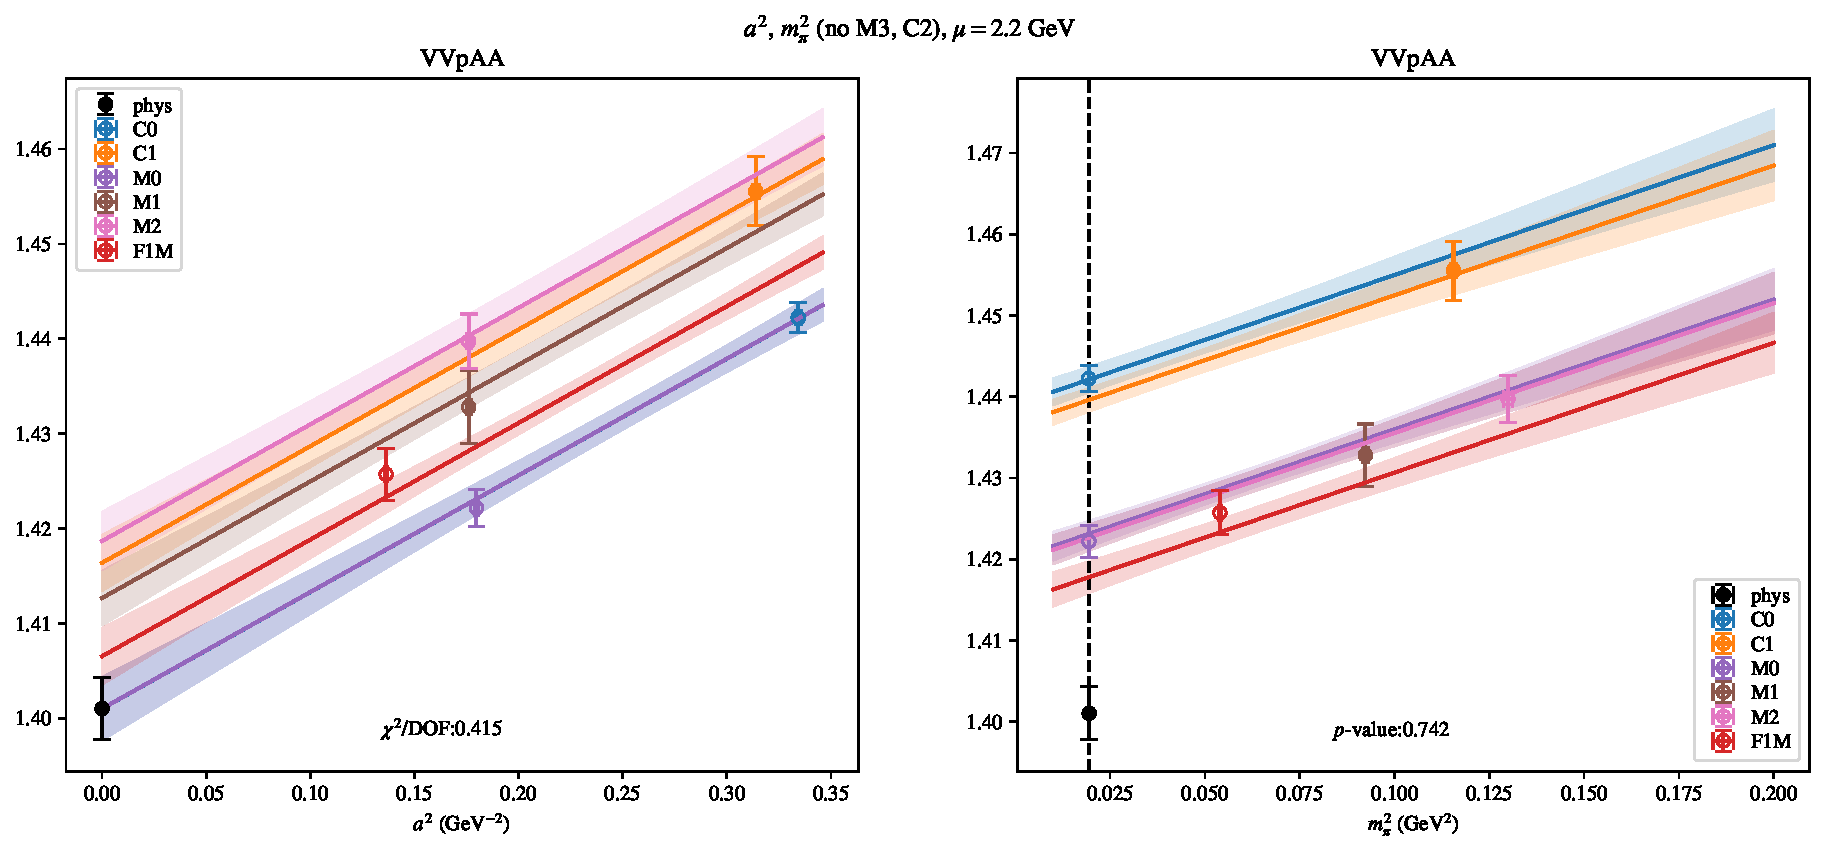
\includepdf[link, pages=-]{VVpAA/NPR/bag_a2m2mcut_22.pdf}
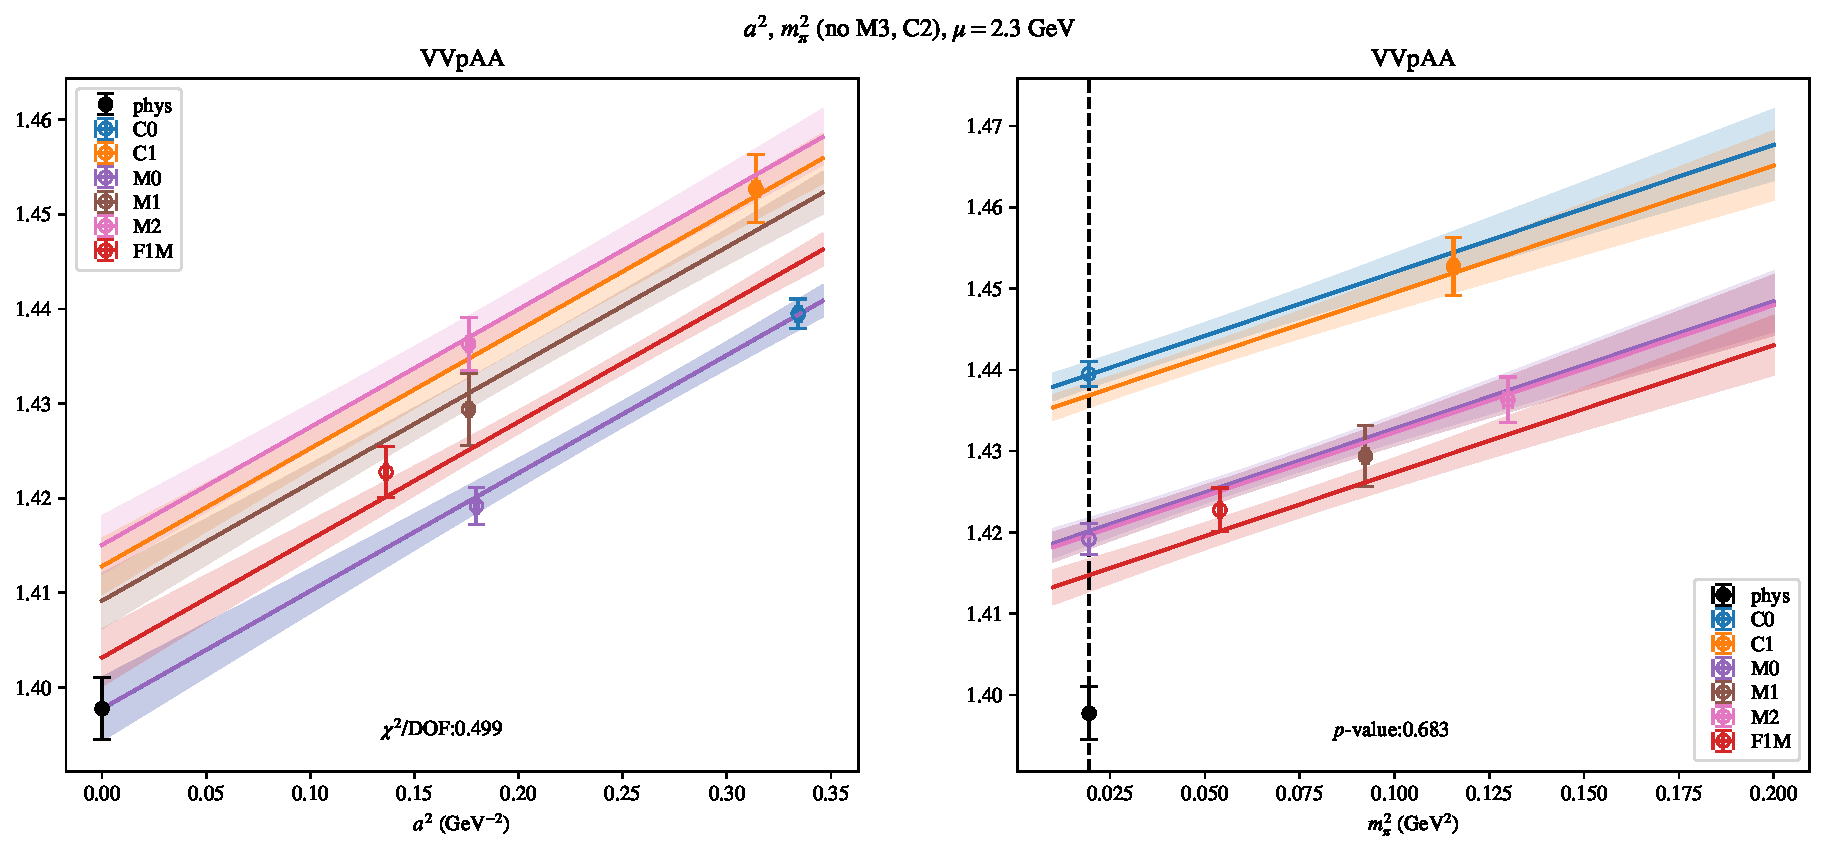
\includepdf[link, pages=-]{VVpAA/NPR/bag_a2m2mcut_23.pdf}
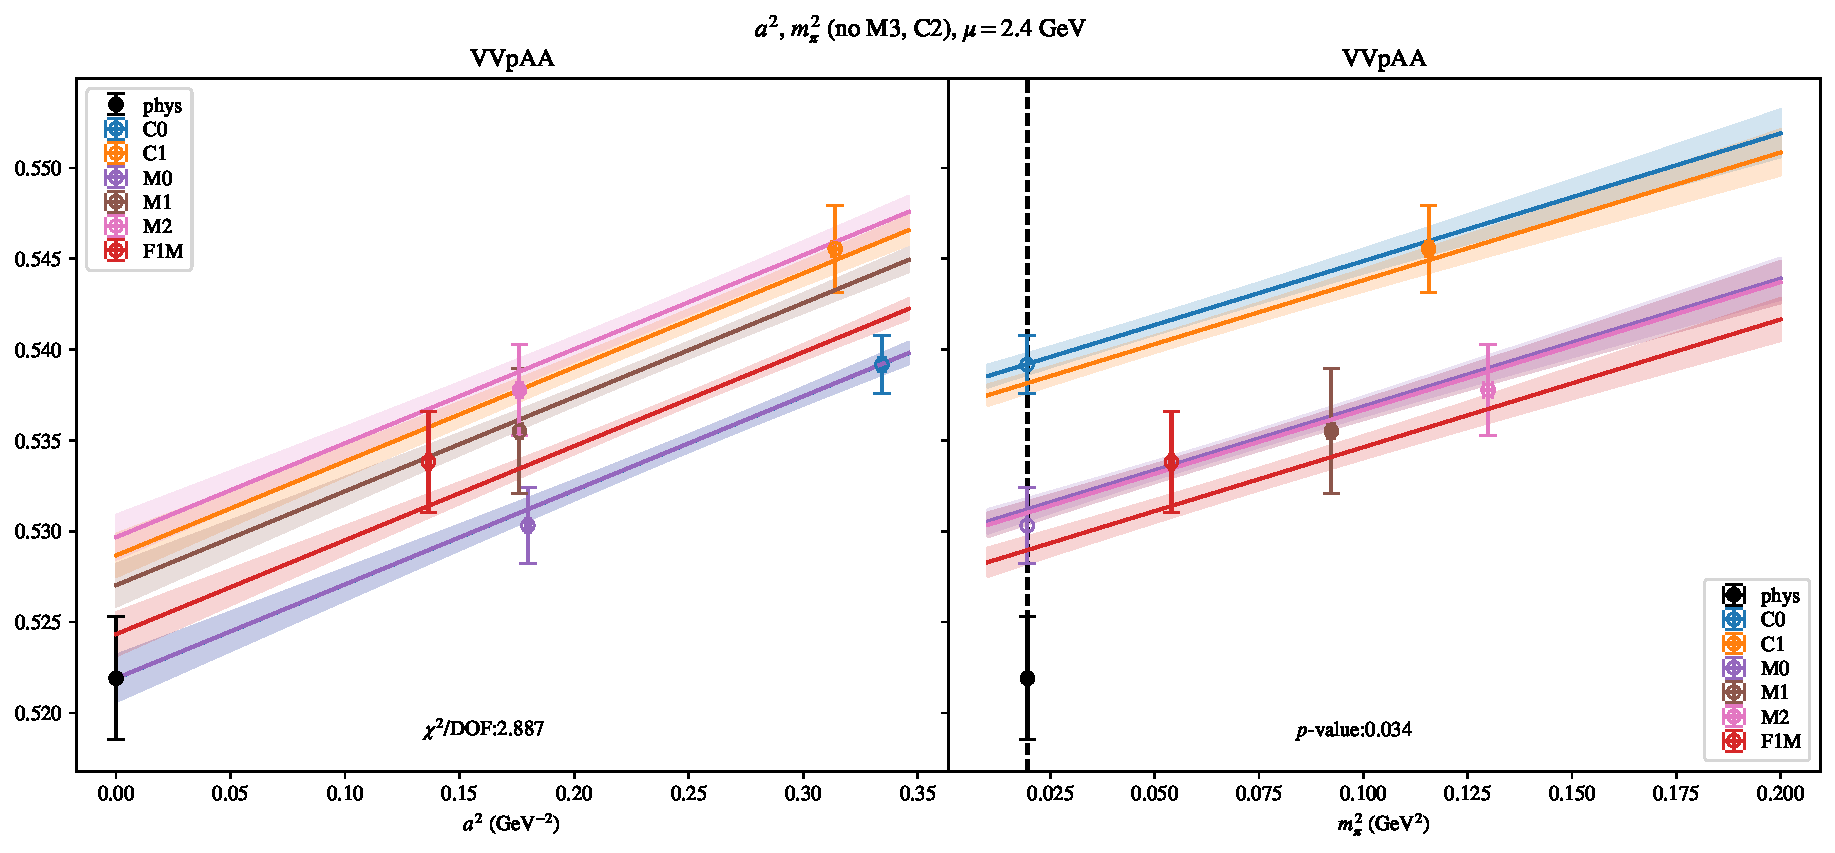
\includepdf[link, pages=-]{VVpAA/NPR/bag_a2m2mcut_24.pdf}
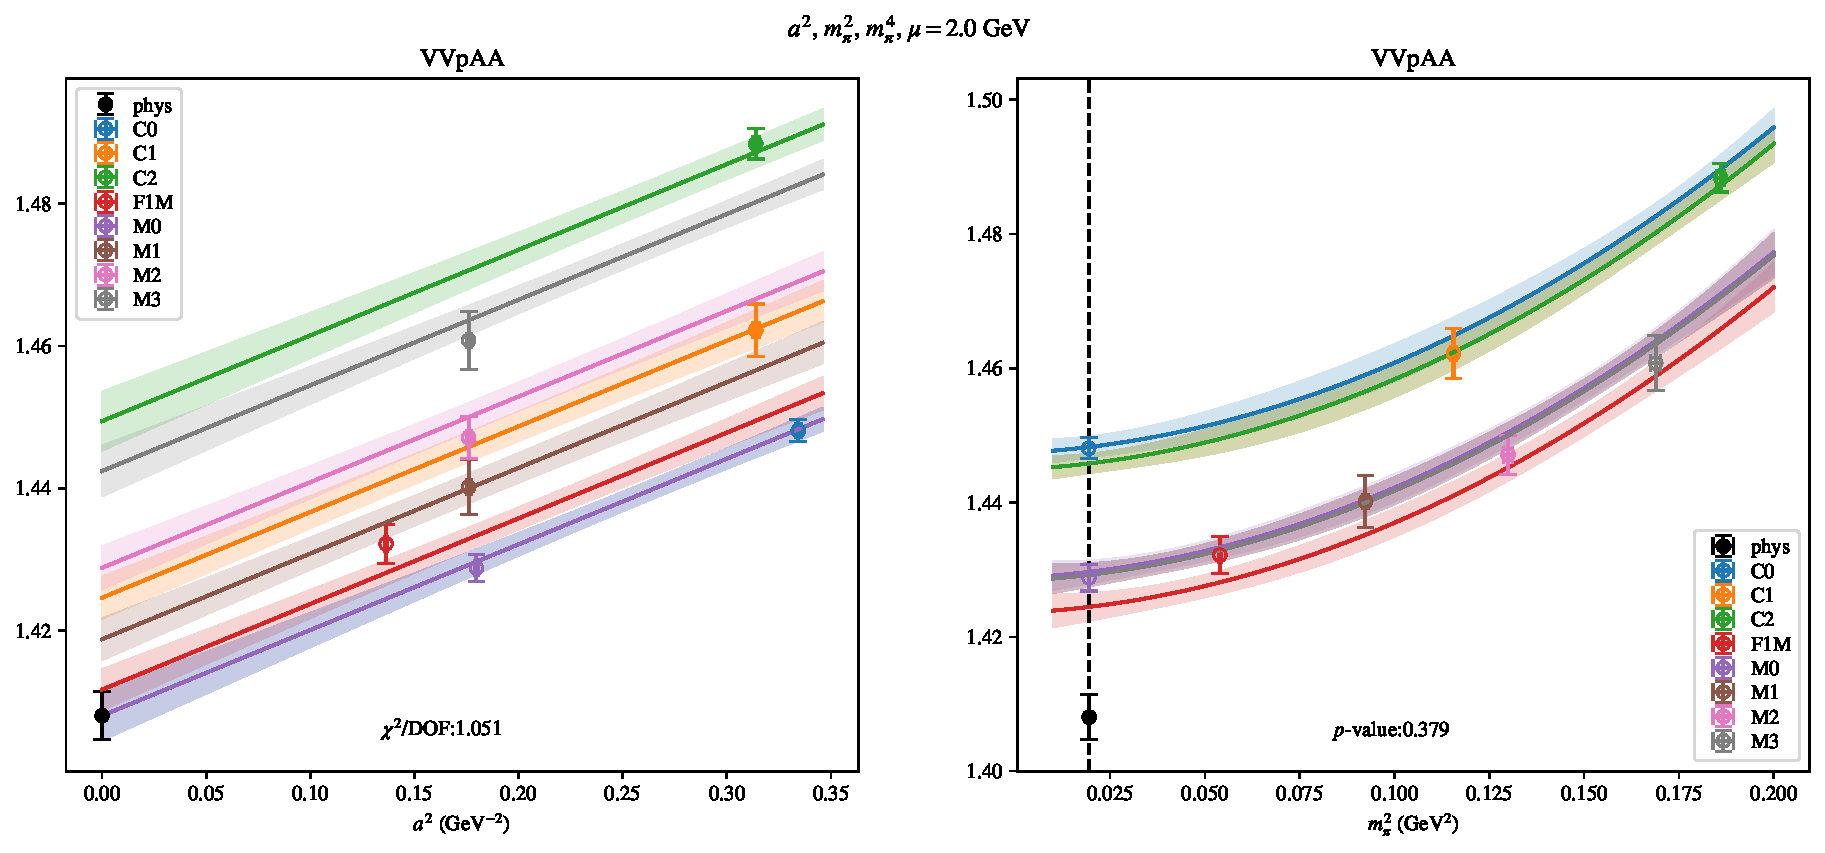
\includepdf[link, pages=-]{VVpAA/NPR/bag_a2m2m4_20.pdf}
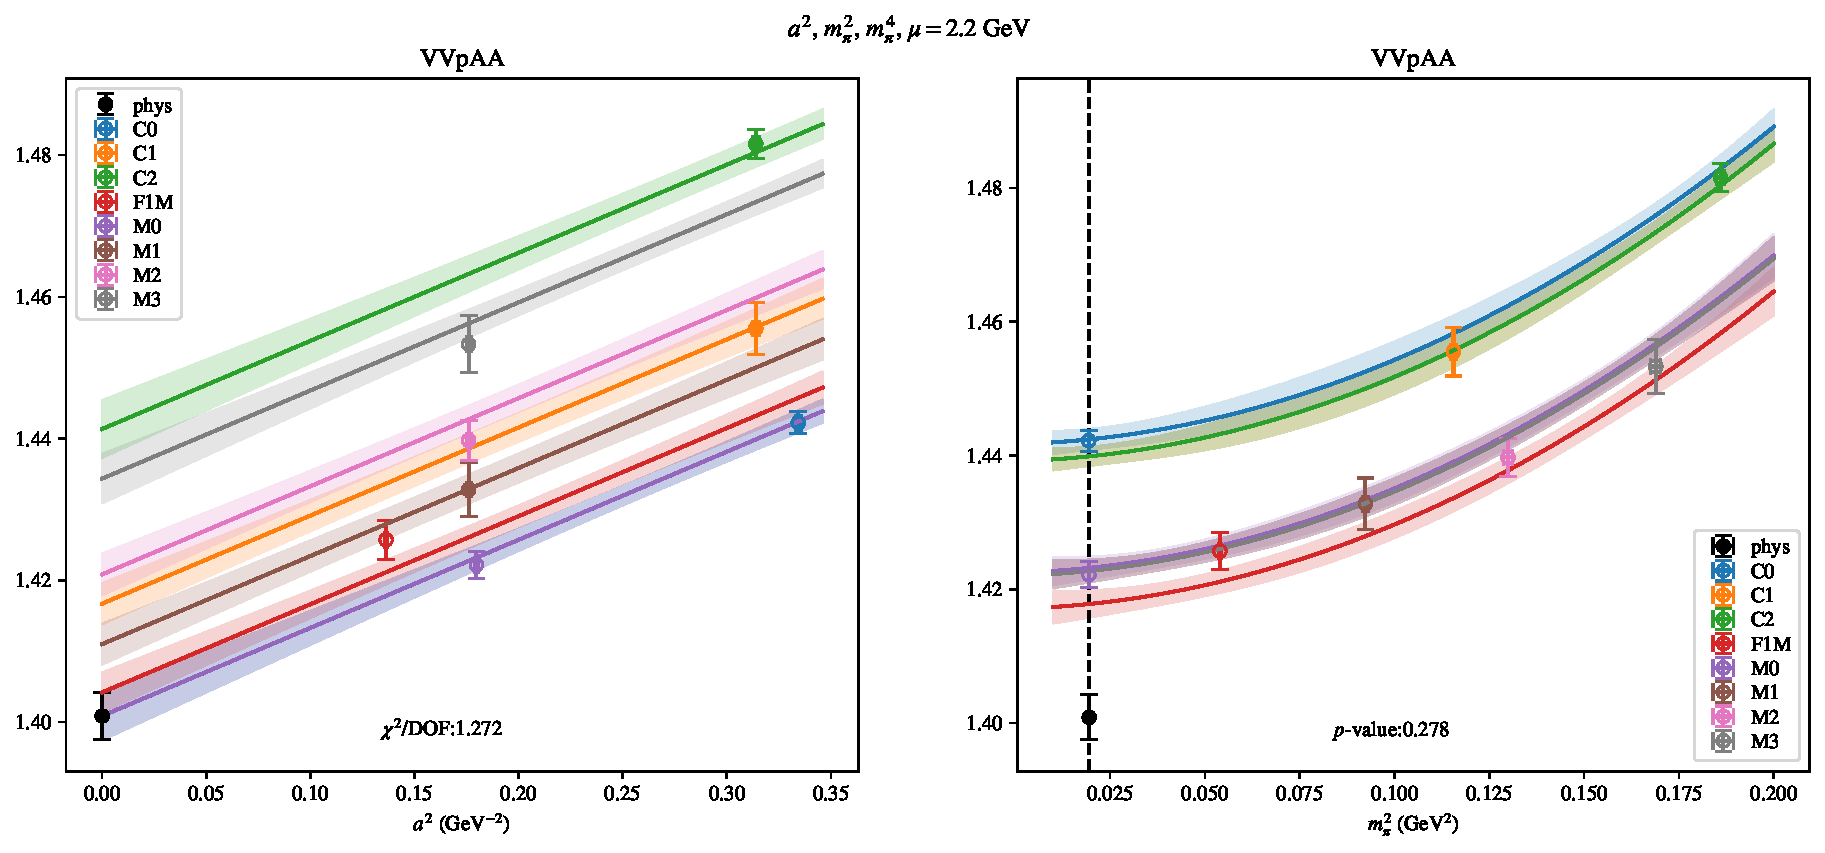
\includepdf[link, pages=-]{VVpAA/NPR/bag_a2m2m4_22.pdf}
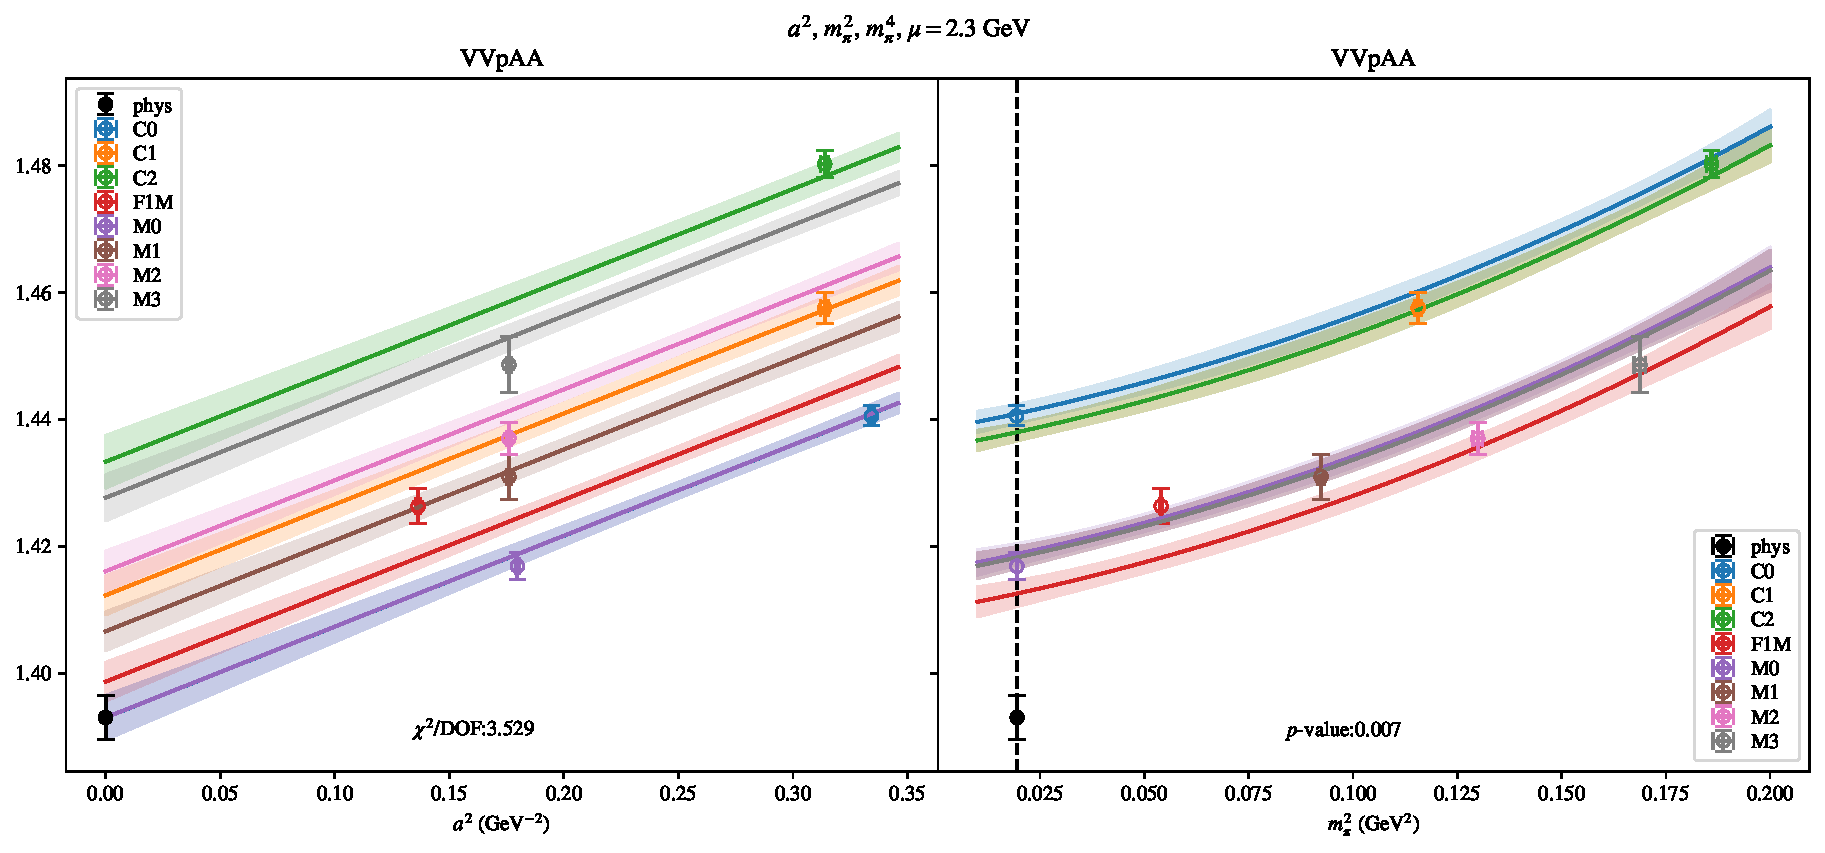
\includepdf[link, pages=-]{VVpAA/NPR/bag_a2m2m4_23.pdf}
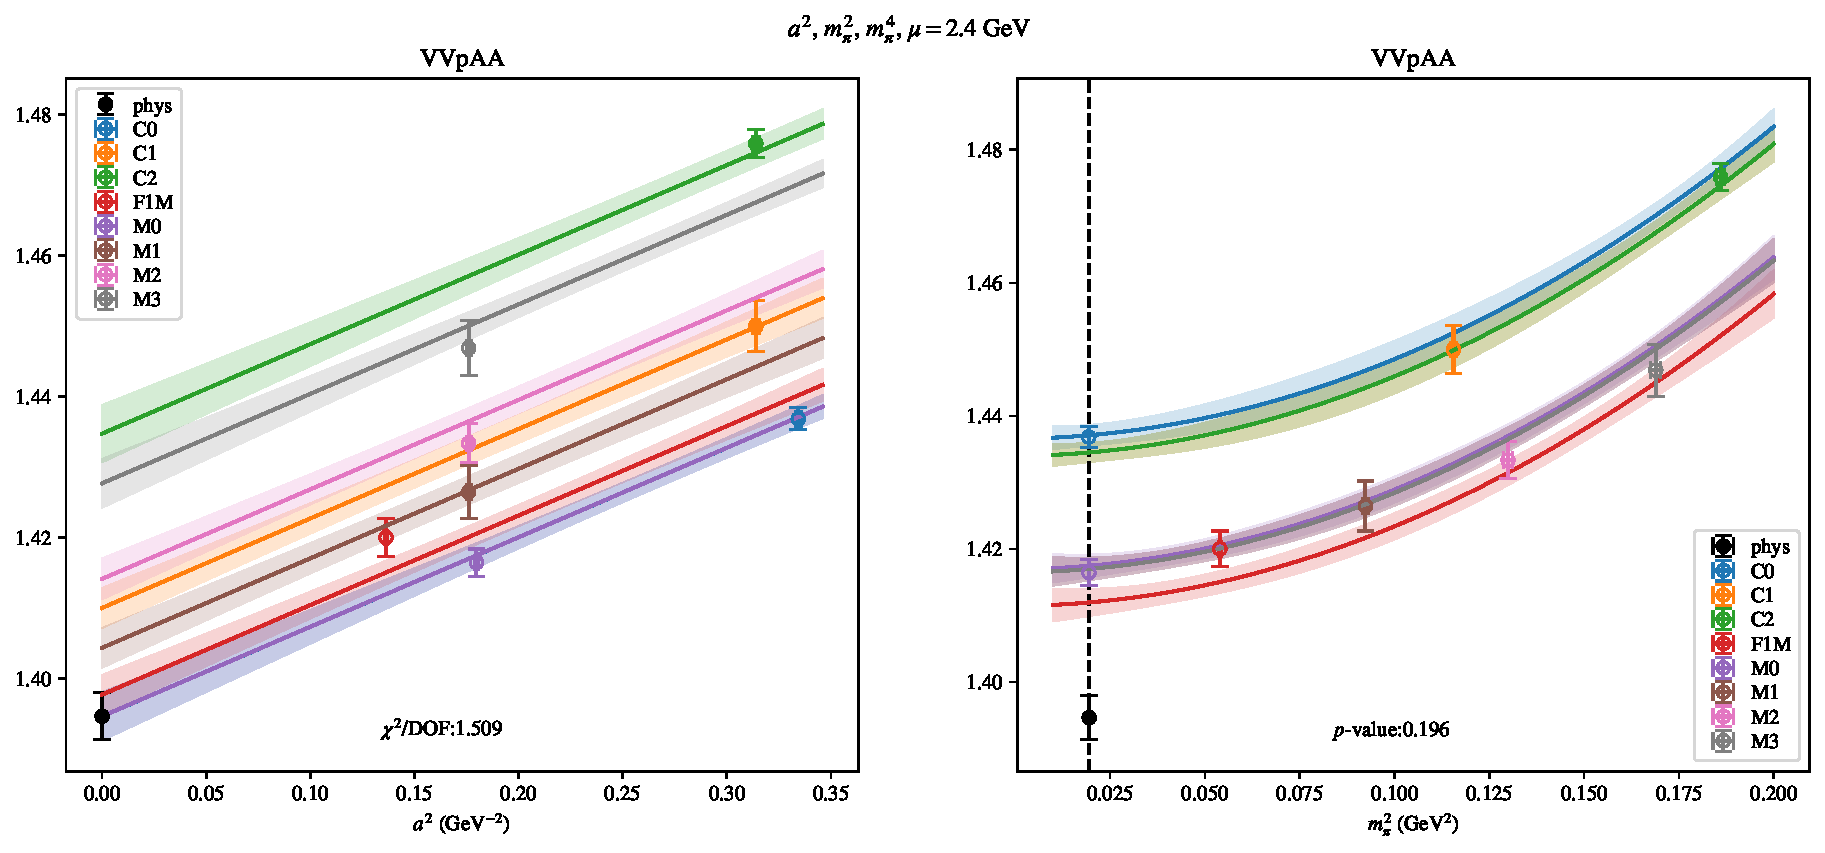
\includepdf[link, pages=-]{VVpAA/NPR/bag_a2m2m4_24.pdf}
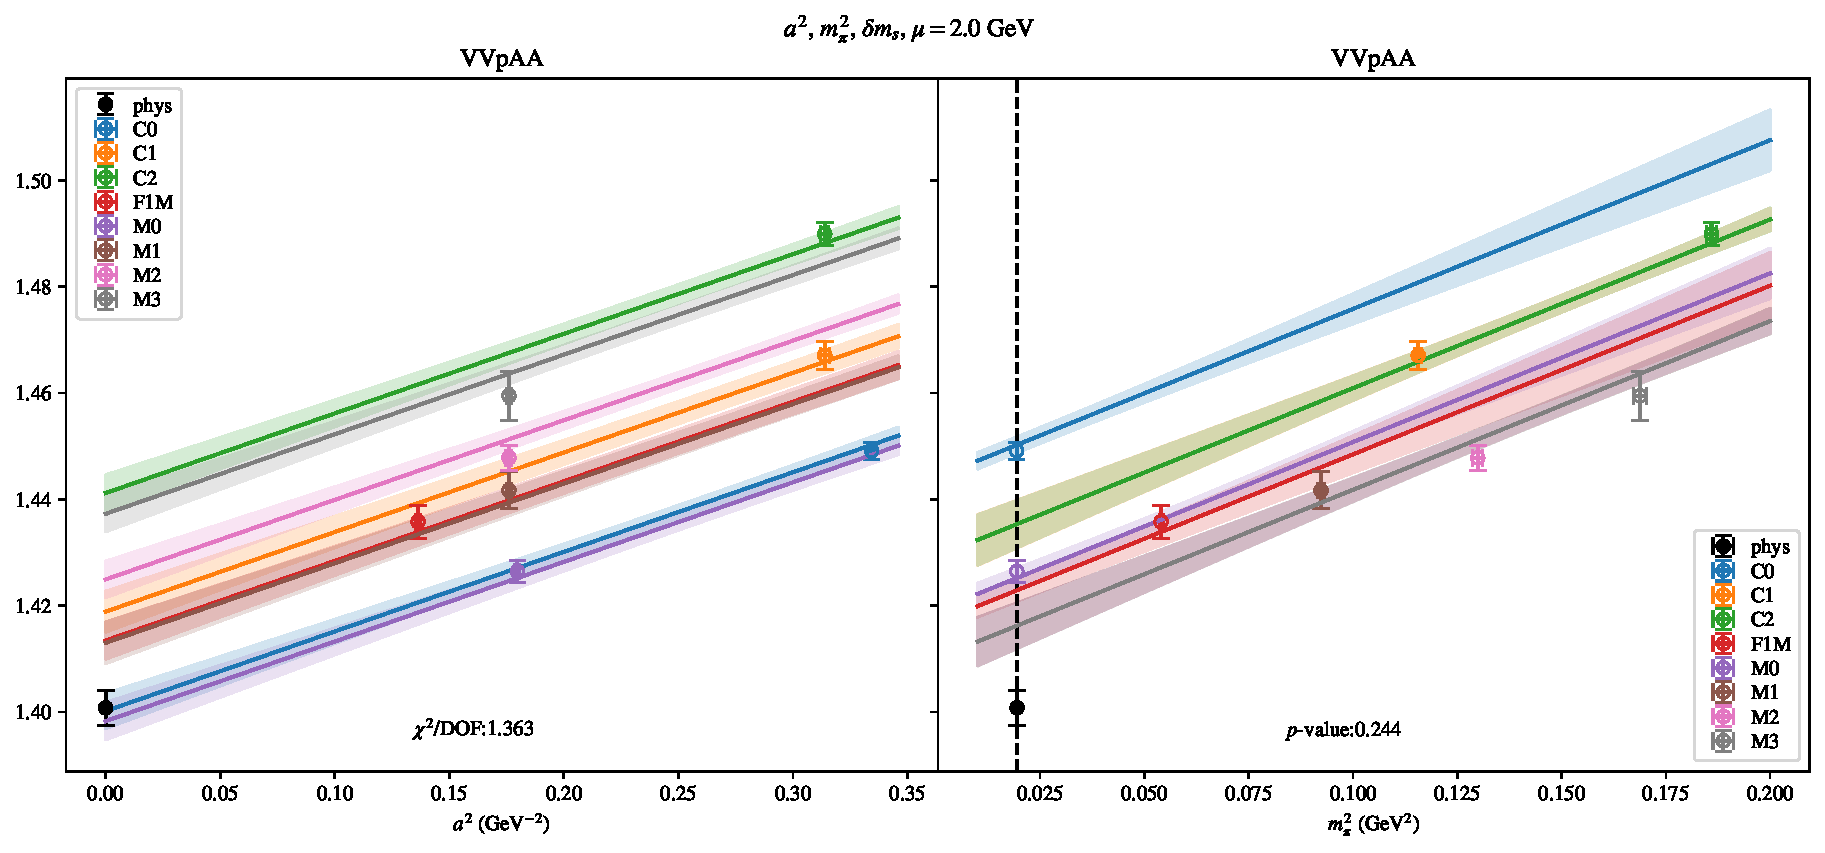
\includepdf[link, pages=-]{VVpAA/NPR/bag_a2m2delm_20.pdf}
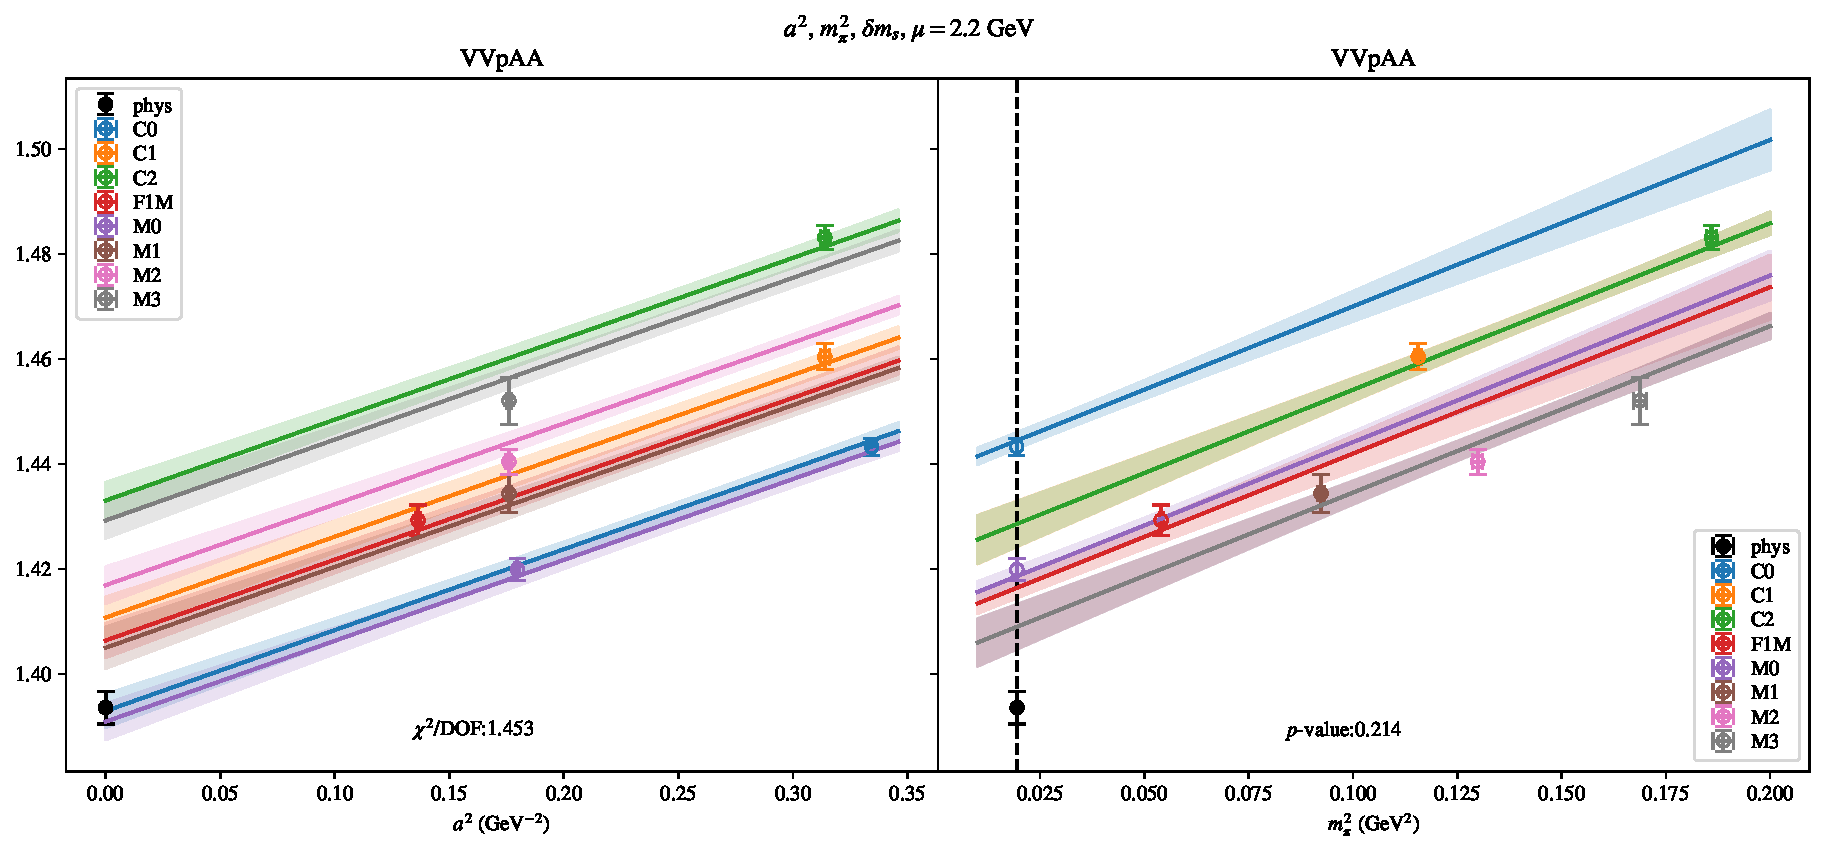
\includepdf[link, pages=-]{VVpAA/NPR/bag_a2m2delm_22.pdf}
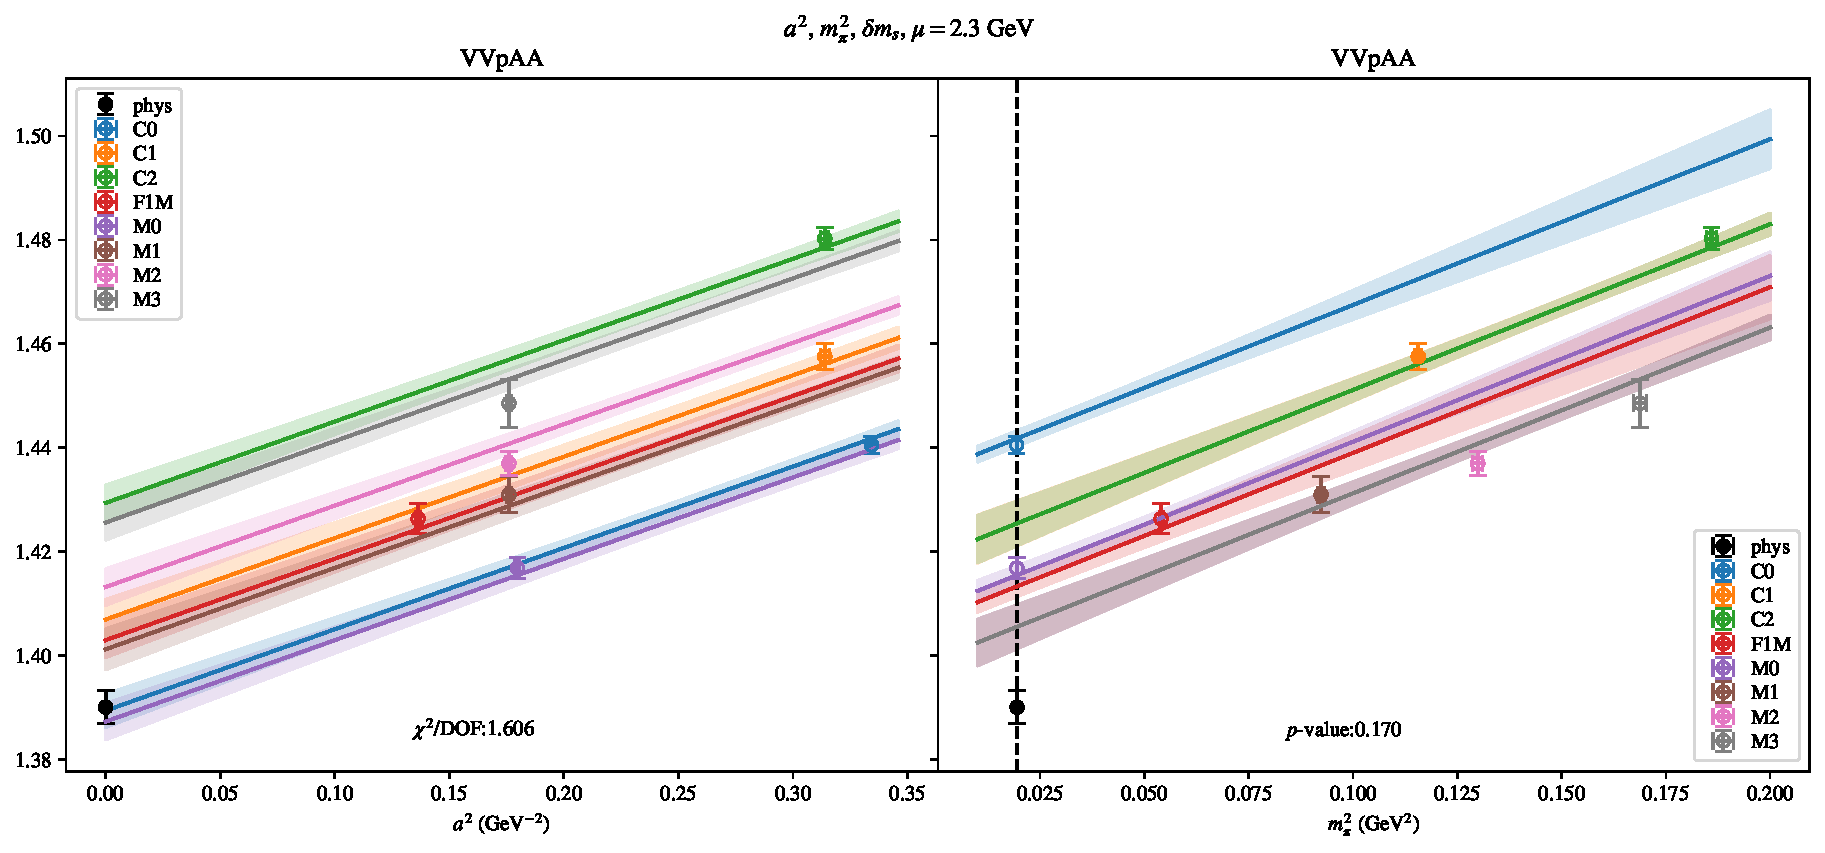
\includepdf[link, pages=-]{VVpAA/NPR/bag_a2m2delm_23.pdf}
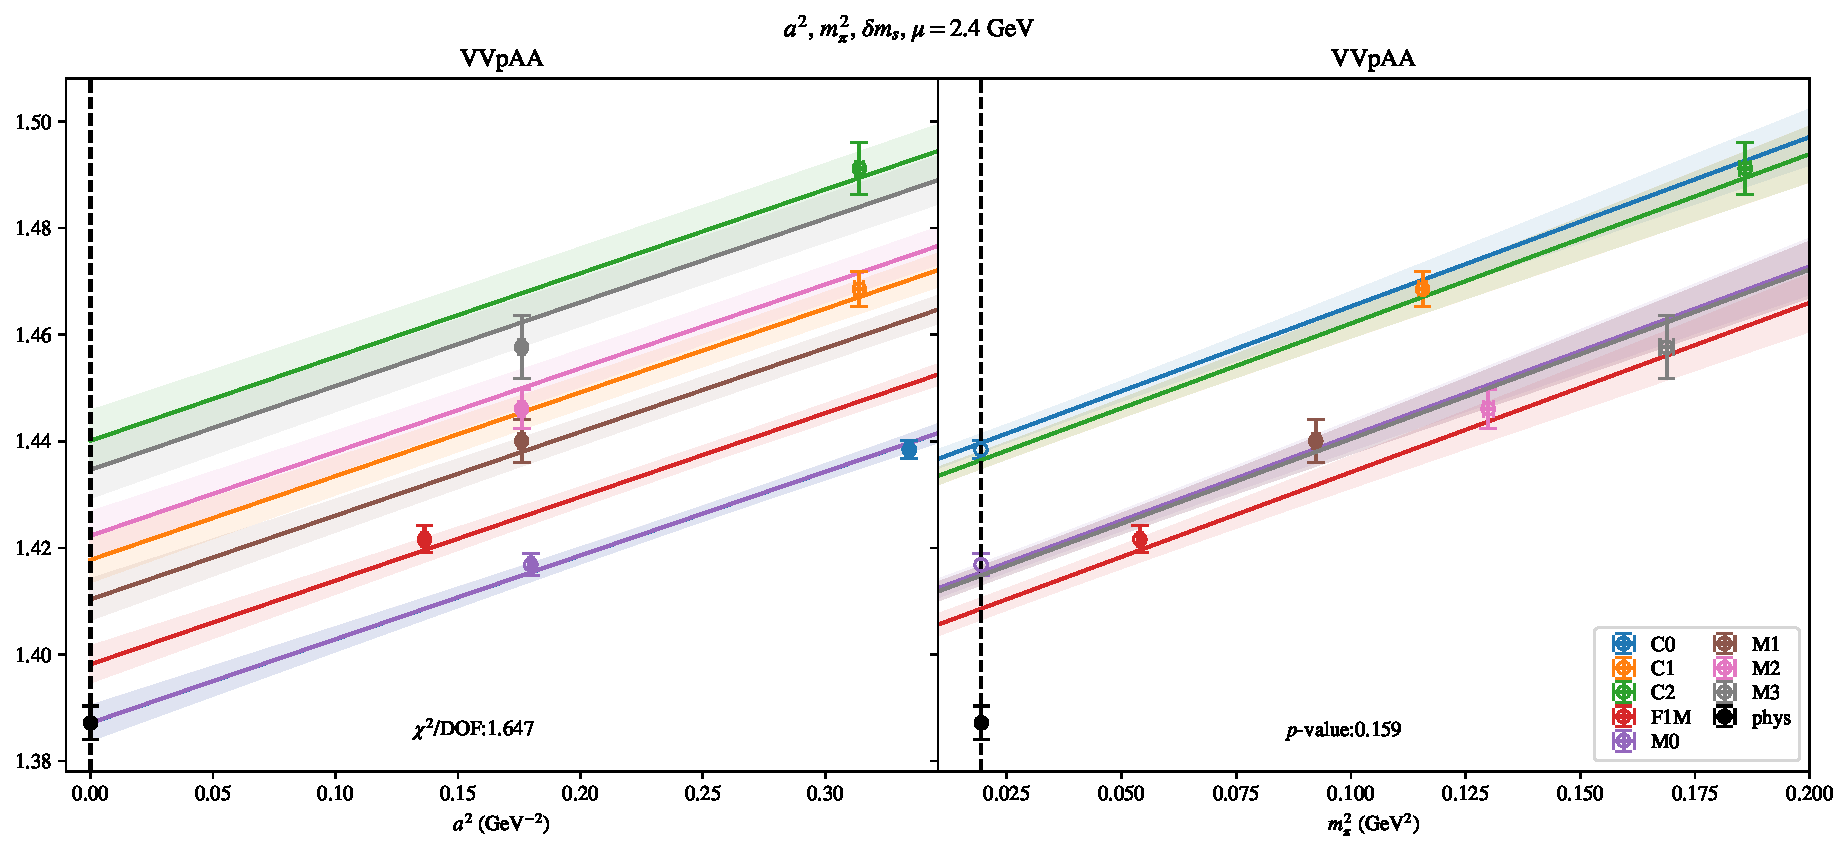
\includepdf[link, pages=-]{VVpAA/NPR/bag_a2m2delm_24.pdf}
\clearpage
\section{$\mathcal{B}_2$}
\begin{table}[h!]
\begin{center}
\begin{tabular}{|c|c|c|c|c|c|c|}
\hline
$\mu$ (GeV) & $a^2$, $m_\pi^2$& $a^2$, $m_\pi^2$ (no C)& $a^2$, $m_\pi^2$, $a^4$& $a^2$, $m_\pi^2$ (no M3, C2)& $a^2$, $m_\pi^2$, $m_\pi^4$& $a^2$, $m_\pi^2$, $\delta m_s$\\
\hline
2.0& \hyperlink{VVmAA/NPR/bag_a2m2_20.pdf.1}{\textbf{-0.9917(15)}: 10.598 (0.0)} & \hyperlink{VVmAA/NPR/bag_a2m2noC_20.pdf.1}{\textbf{-0.9310(87)}: 1.871 (0.154)} & \hyperlink{VVmAA/NPR/bag_a2a4m2_20.pdf.1}{\textbf{-0.898(12)}: 1.909 (0.106)} & \hyperlink{VVmAA/NPR/bag_a2m2mcut_20.pdf.1}{\textbf{-0.9923(15)}: 16.526 (0.0)} & \hyperlink{VVmAA/NPR/bag_a2m2m4_20.pdf.1}{\textbf{-0.9936(15)}: 10.104 (0.0)} & \hyperlink{VVmAA/NPR/bag_a2m2delm_20.pdf.1}{\textbf{-0.9942(15)}: 2.092 (0.079)}\\
2.2& \hyperlink{VVmAA/NPR/bag_a2m2_22.pdf.1}{\textbf{-1.0061(14)}: 10.271 (0.0)} & \hyperlink{VVmAA/NPR/bag_a2m2noC_22.pdf.1}{\textbf{-0.9498(86)}: 2.933 (0.053)} & \hyperlink{VVmAA/NPR/bag_a2a4m2_22.pdf.1}{\textbf{-0.919(12)}: 2.581 (0.035)} & \hyperlink{VVmAA/NPR/bag_a2m2mcut_22.pdf.1}{\textbf{-1.0068(14)}: 14.456 (0.0)} & \hyperlink{VVmAA/NPR/bag_a2m2m4_22.pdf.1}{\textbf{-1.0081(14)}: 8.637 (0.0)} & \hyperlink{VVmAA/NPR/bag_a2m2delm_22.pdf.1}{\textbf{-1.0082(15)}: 3.258 (0.011)}\\
2.3& \hyperlink{VVmAA/NPR/bag_a2m2_23.pdf.1}{\textbf{-1.0122(14)}: 10.049 (0.0)} & \hyperlink{VVmAA/NPR/bag_a2m2noC_23.pdf.1}{\textbf{-0.9571(85)}: 3.084 (0.046)} & \hyperlink{VVmAA/NPR/bag_a2a4m2_23.pdf.1}{\textbf{-0.927(12)}: 2.444 (0.044)} & \hyperlink{VVmAA/NPR/bag_a2m2mcut_23.pdf.1}{\textbf{-1.0127(14)}: 14.407 (0.0)} & \hyperlink{VVmAA/NPR/bag_a2m2m4_23.pdf.1}{\textbf{-1.0141(14)}: 8.861 (0.0)} & \hyperlink{VVmAA/NPR/bag_a2m2delm_23.pdf.1}{\textbf{-1.0142(14)}: 3.181 (0.013)}\\
2.4& \hyperlink{VVmAA/NPR/bag_a2m2_24.pdf.1}{\textbf{-1.0170(14)}: 9.421 (0.0)} & \hyperlink{VVmAA/NPR/bag_a2m2noC_24.pdf.1}{\textbf{-0.9642(84)}: 3.135 (0.044)} & \hyperlink{VVmAA/NPR/bag_a2a4m2_24.pdf.1}{\textbf{-0.937(12)}: 2.622 (0.033)} & \hyperlink{VVmAA/NPR/bag_a2m2mcut_24.pdf.1}{\textbf{-1.0174(14)}: 13.378 (0.0)} & \hyperlink{VVmAA/NPR/bag_a2m2m4_24.pdf.1}{\textbf{-1.0189(14)}: 8.42 (0.0)} & \hyperlink{VVmAA/NPR/bag_a2m2delm_24.pdf.1}{\textbf{-1.0189(14)}: 3.056 (0.016)}\\
\hline
\end{tabular}
\caption{Physical point value from chiral and continuum extrapolation at renormalisation scale $\mu$. Entries are \textbf{value(error)}: $\chi^2/\text{DOF}$ ($p$-value).}
\end{center}
\end{table}
\begin{table}[h!]
\begin{center}
\begin{tabular}{|c c|c|c|c|c|c|c|}
\hline
$\mu$ (GeV) &  & $a^2$, $m_\pi^2$& $a^2$, $m_\pi^2$ (no C)& $a^2$, $m_\pi^2$, $a^4$& $a^2$, $m_\pi^2$ (no M3, C2)& $a^2$, $m_\pi^2$, $m_\pi^4$& $a^2$, $m_\pi^2$, $\delta m_s$\\
\hline
\multirow{3}{0.5in}{2.0} & $\alpha$ & 0.1815(55)& -0.167(49)& -0.65(11)& 0.1830(54)& 0.1873(55)& 0.1909(56)\\
 & $\beta$ & -0.00104(14)& -0.00106(23)& -0.00075(14)& -0.00068(24)& 0.00149(71)& -0.00070(14)\\
 & $\gamma$ &  &  & 1.65(22)&  & -0.000232(63)& -0.0146(20)\\
\hline
\multirow{3}{0.5in}{2.2} & $\alpha$ & 0.2258(53)& -0.097(49)& -0.54(11)& 0.2275(53)& 0.2321(53)& 0.2340(55)\\
 & $\beta$ & -0.00118(12)& -0.00114(21)& -0.00091(13)& -0.00067(22)& 0.00150(65)& -0.00088(13)\\
 & $\gamma$ &  &  & 1.52(22)&  & -0.000243(57)& -0.0132(20)\\
\hline
\multirow{3}{0.5in}{2.3} & $\alpha$ & 0.2491(52)& -0.066(48)& -0.50(11)& 0.2505(53)& 0.2553(53)& 0.2570(54)\\
 & $\beta$ & -0.00118(12)& -0.00115(20)& -0.00091(13)& -0.00072(22)& 0.00127(63)& -0.00088(13)\\
 & $\gamma$ &  &  & 1.50(22)&  & -0.000222(56)& -0.0129(20)\\
\hline
\multirow{3}{0.5in}{2.4} & $\alpha$ & 0.2706(52)& -0.032(48)& -0.44(11)& 0.2715(53)& 0.2767(53)& 0.2781(53)\\
 & $\beta$ & -0.00115(12)& -0.00116(19)& -0.00090(13)& -0.00072(21)& 0.00113(61)& -0.00086(13)\\
 & $\gamma$ &  &  & 1.41(22)&  & -0.000206(54)& -0.0122(20)\\
\hline
\end{tabular}
\caption{Fit values of coefficients in $Q = Q_{phys} + \mathbf{\alpha} a^2 + \mathbf{\beta}\left(\frac{m_\pi^2}{f_\pi^2}-\frac{m_{\pi,PDG}^2}{f_\pi^2}\right) + \gamma(\ldots)$}
\end{center}
\end{table}
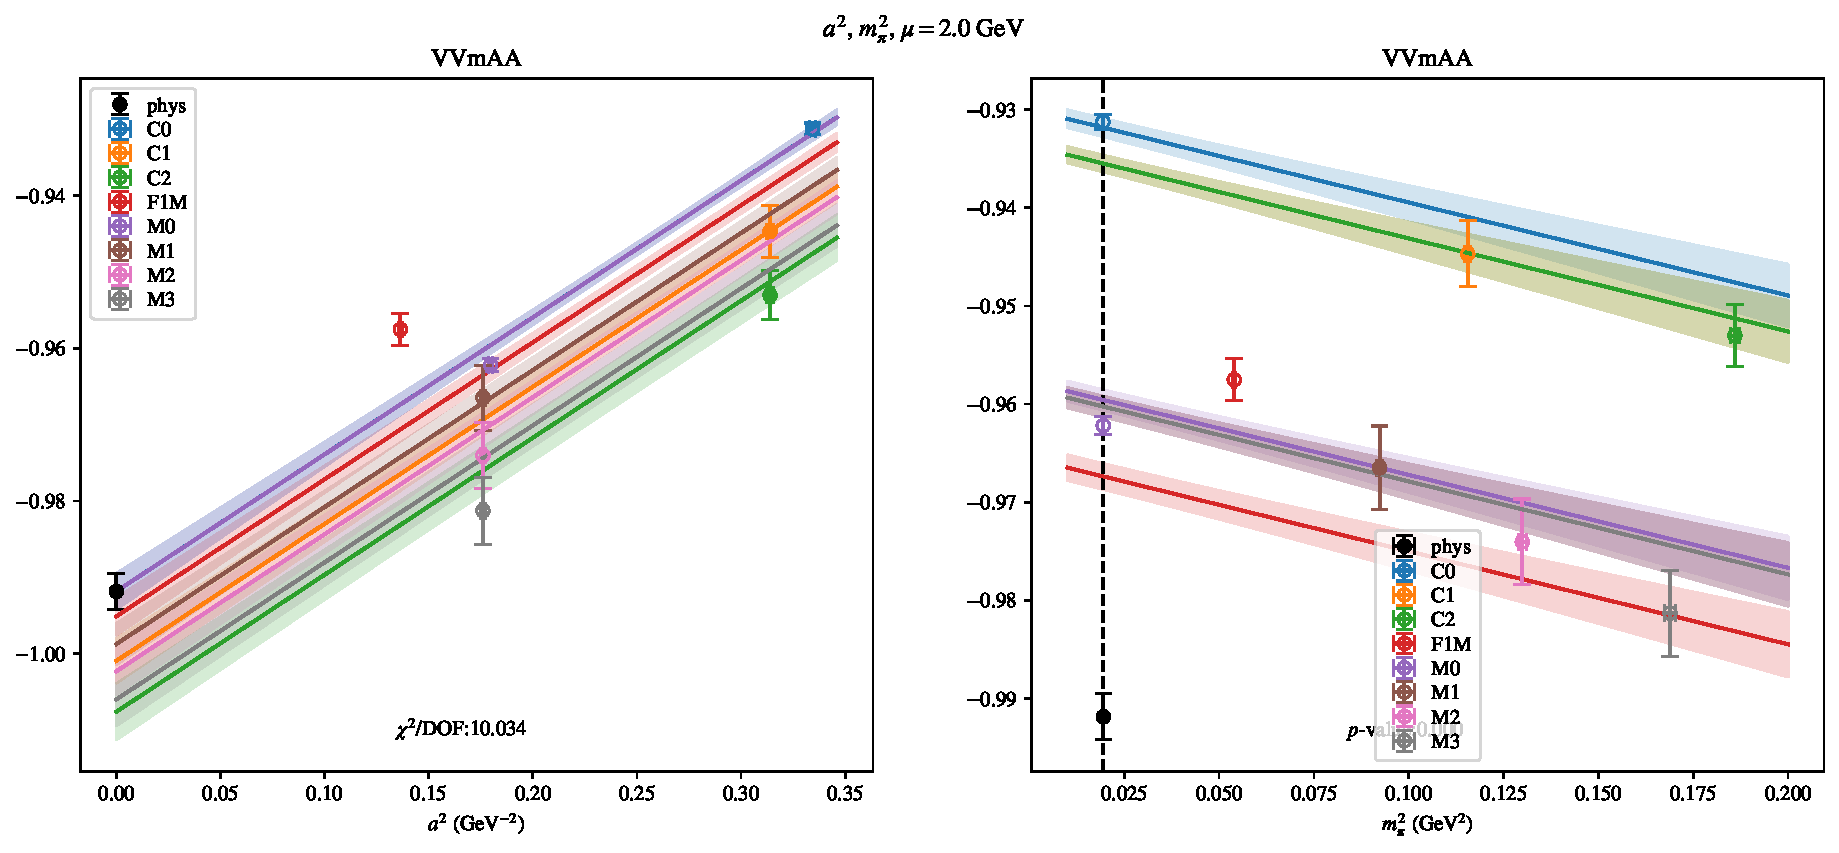
\includepdf[link, pages=-]{VVmAA/NPR/bag_a2m2_20.pdf}
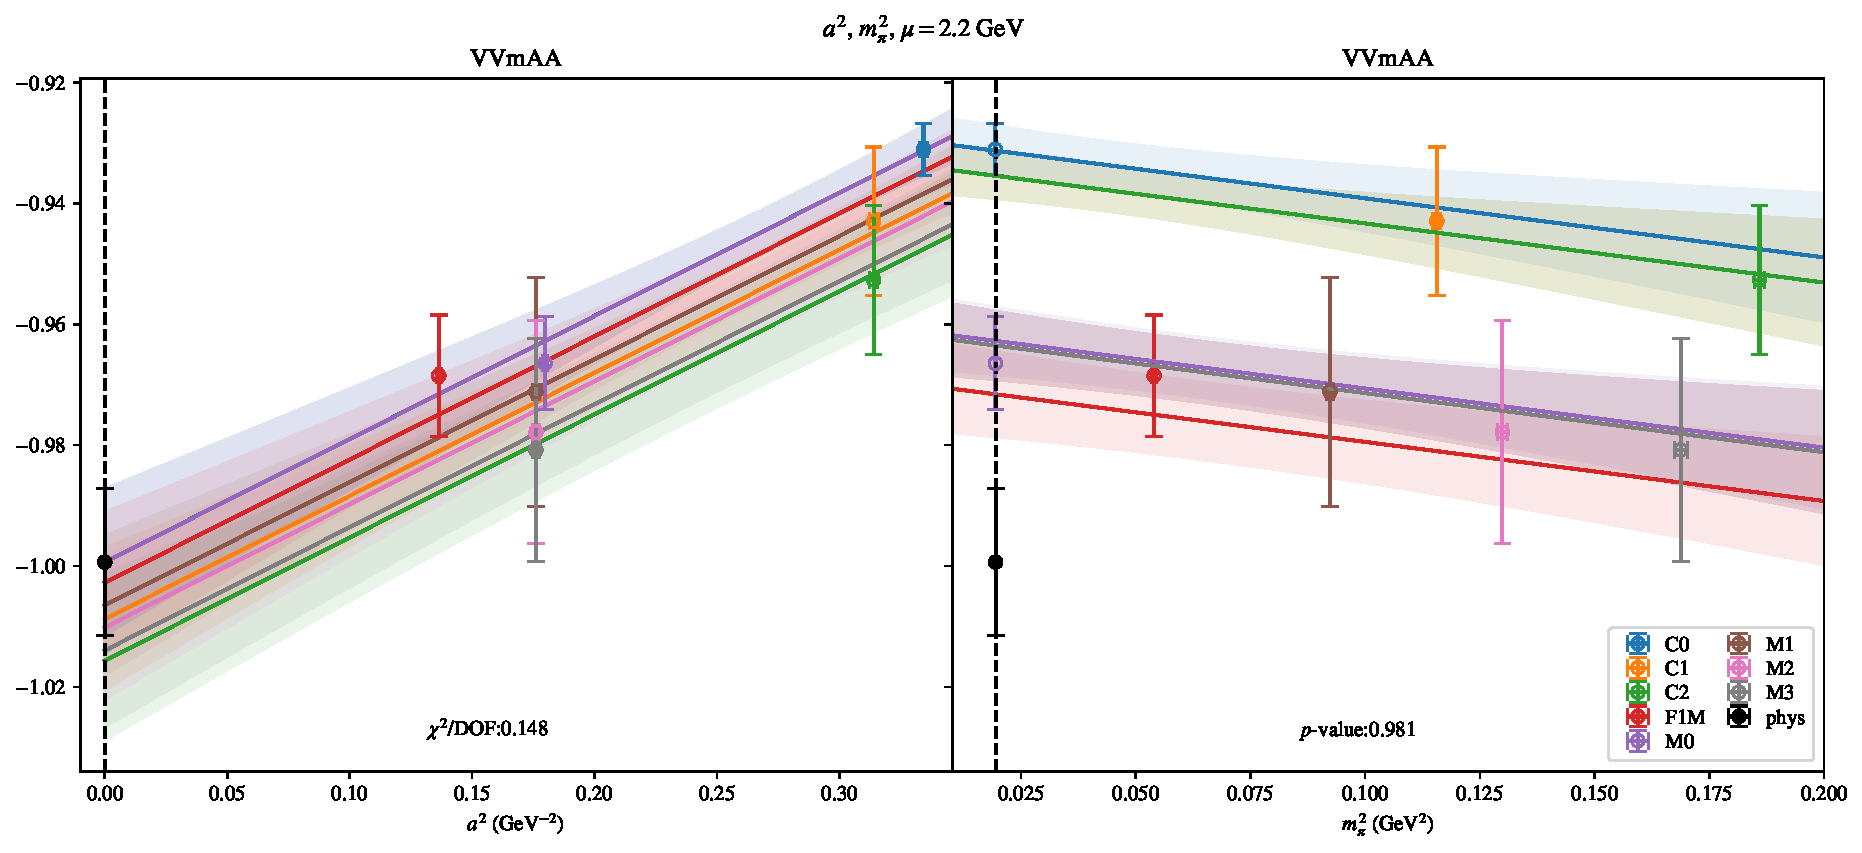
\includepdf[link, pages=-]{VVmAA/NPR/bag_a2m2_22.pdf}
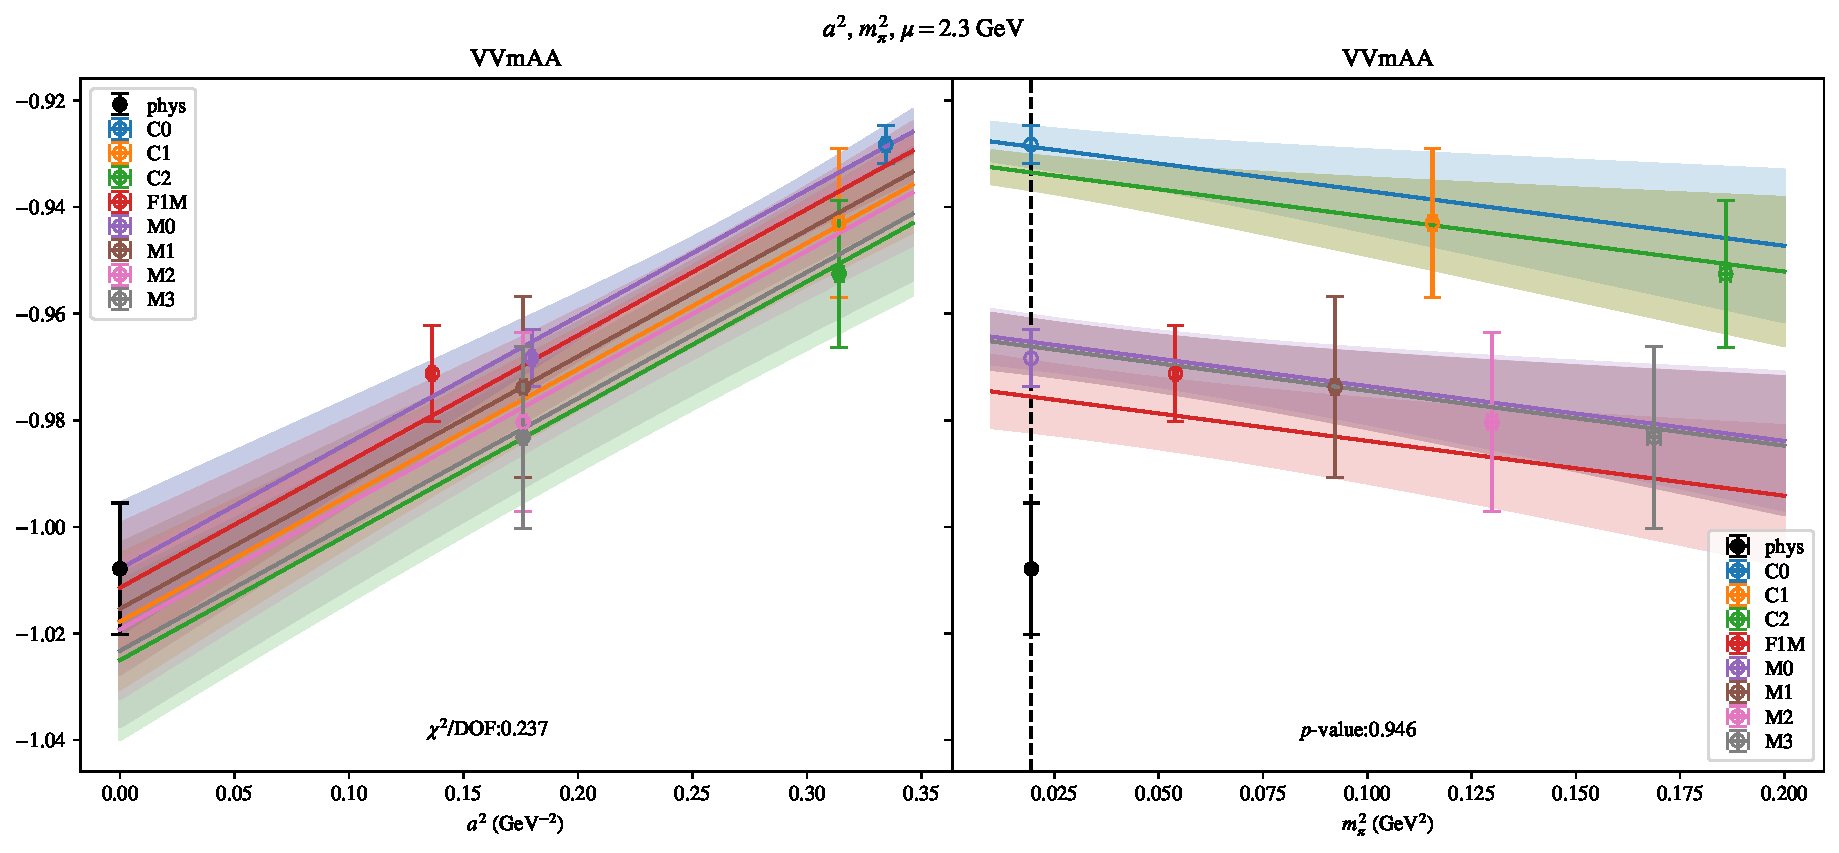
\includepdf[link, pages=-]{VVmAA/NPR/bag_a2m2_23.pdf}
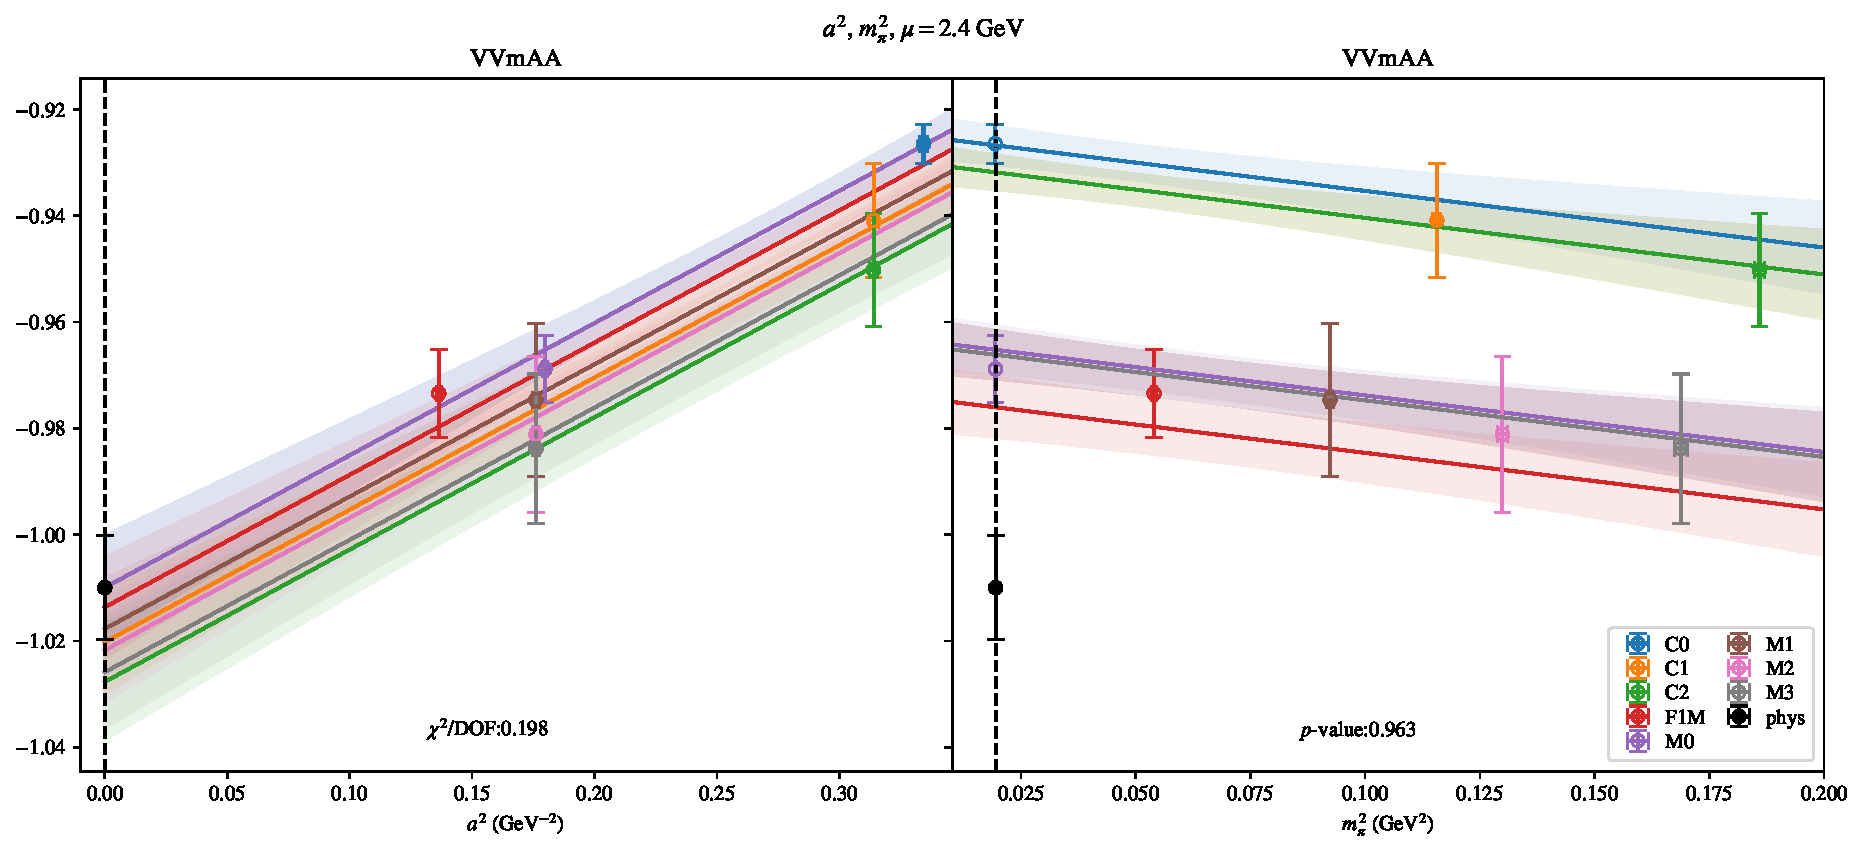
\includepdf[link, pages=-]{VVmAA/NPR/bag_a2m2_24.pdf}
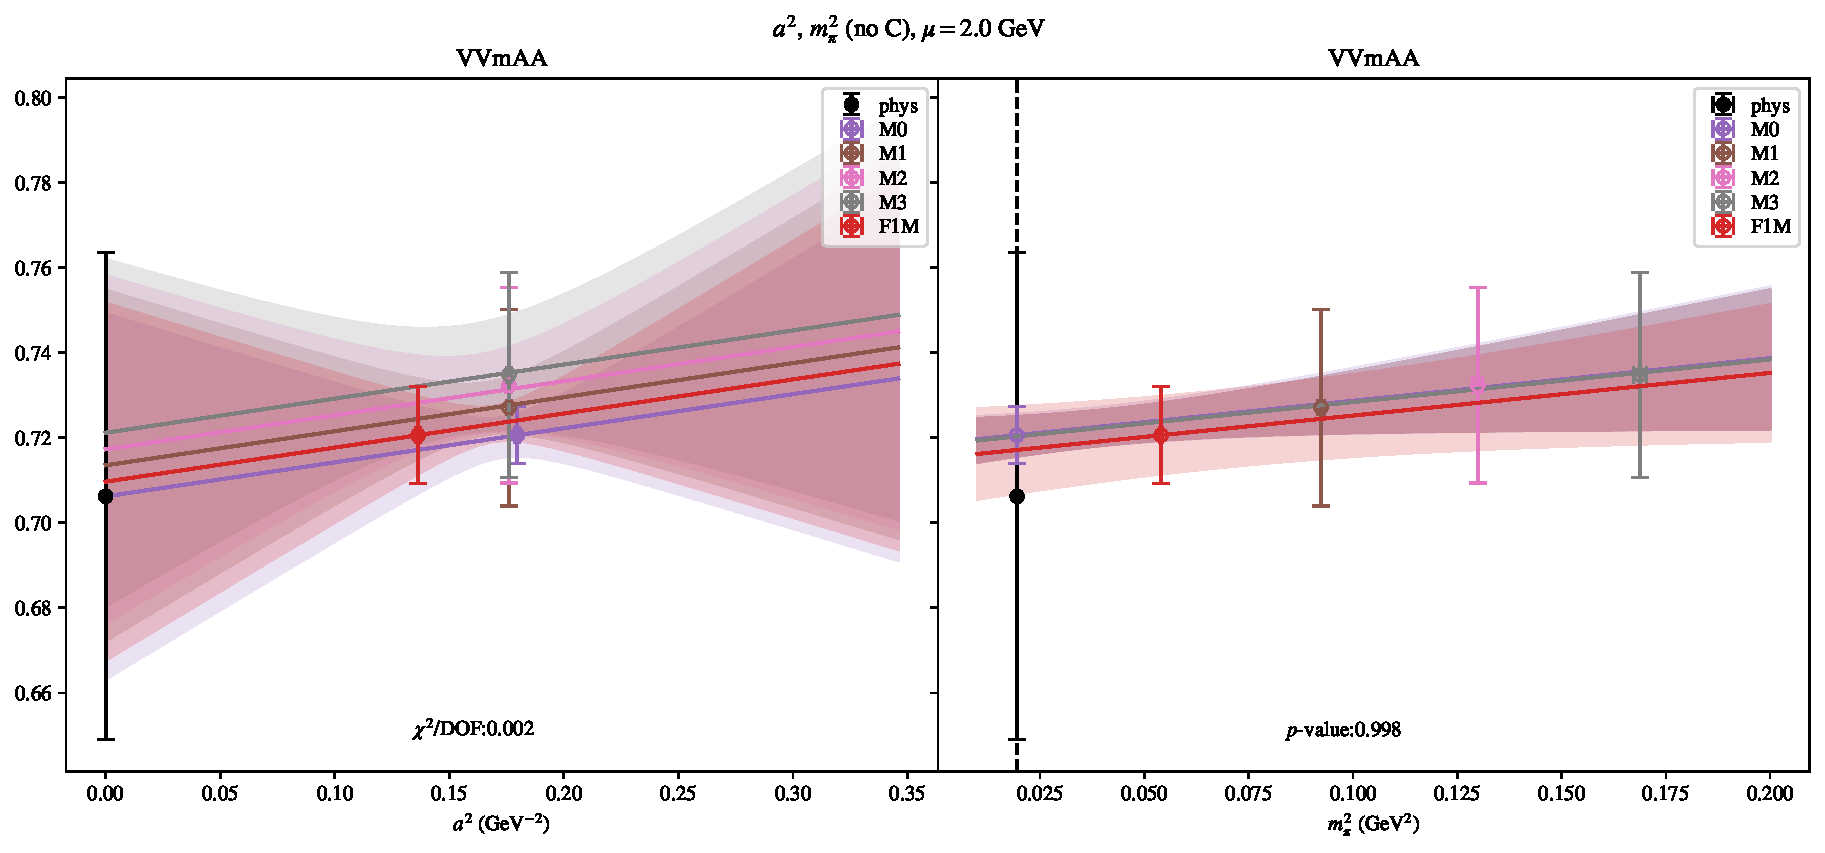
\includepdf[link, pages=-]{VVmAA/NPR/bag_a2m2noC_20.pdf}
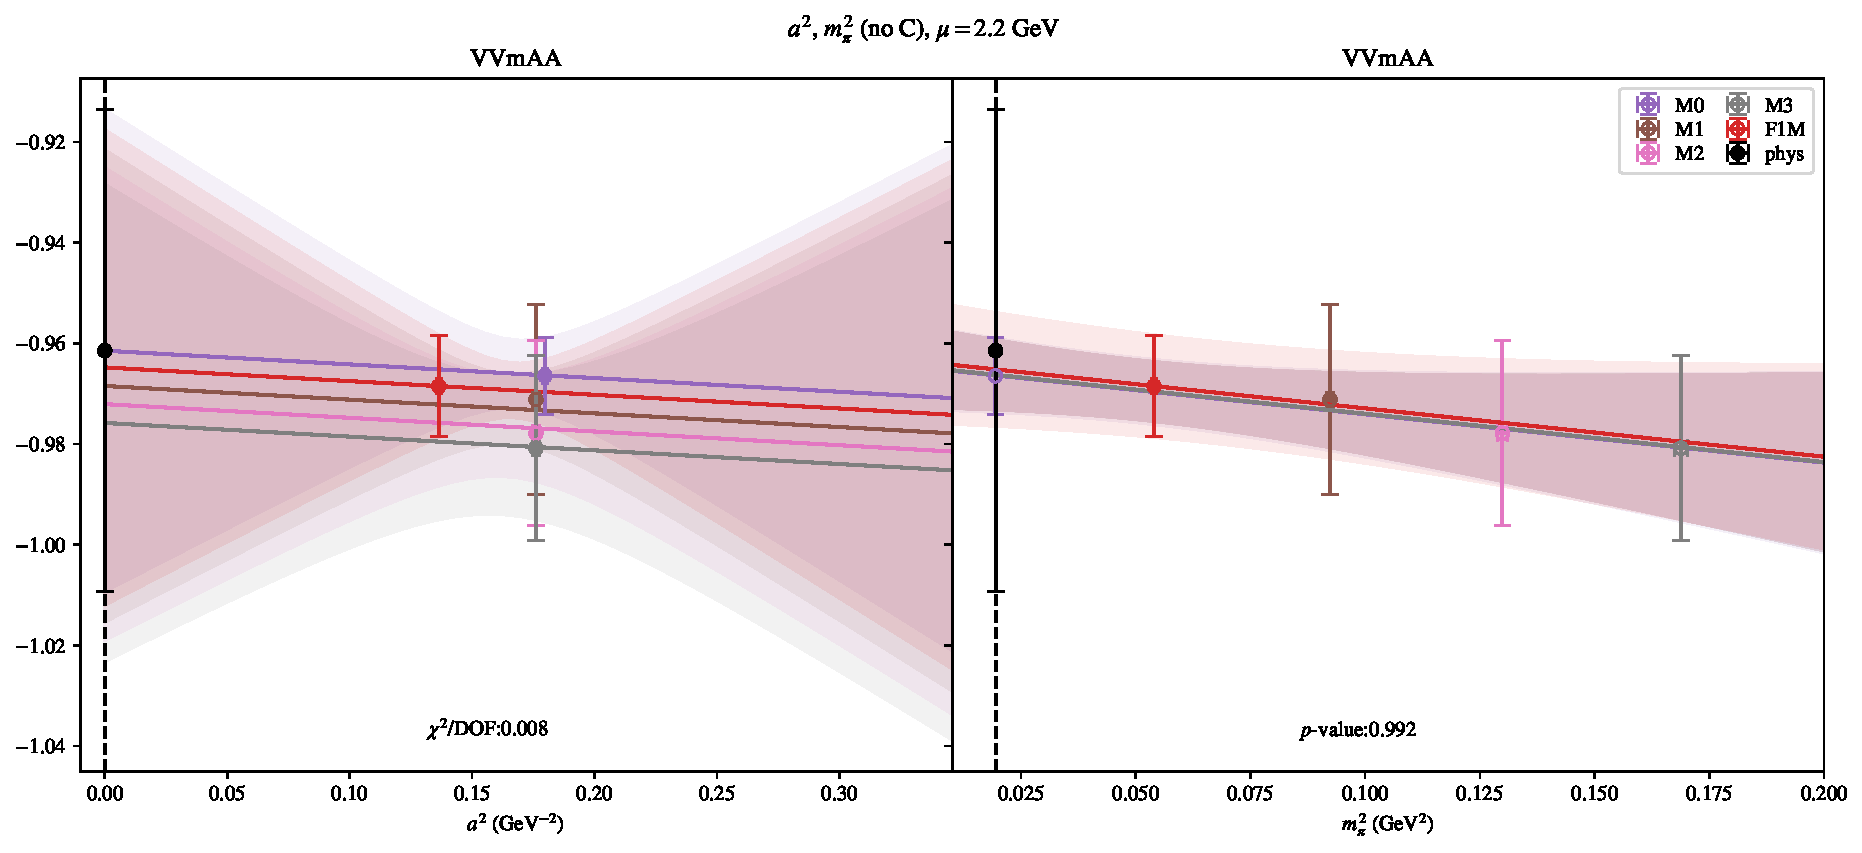
\includepdf[link, pages=-]{VVmAA/NPR/bag_a2m2noC_22.pdf}
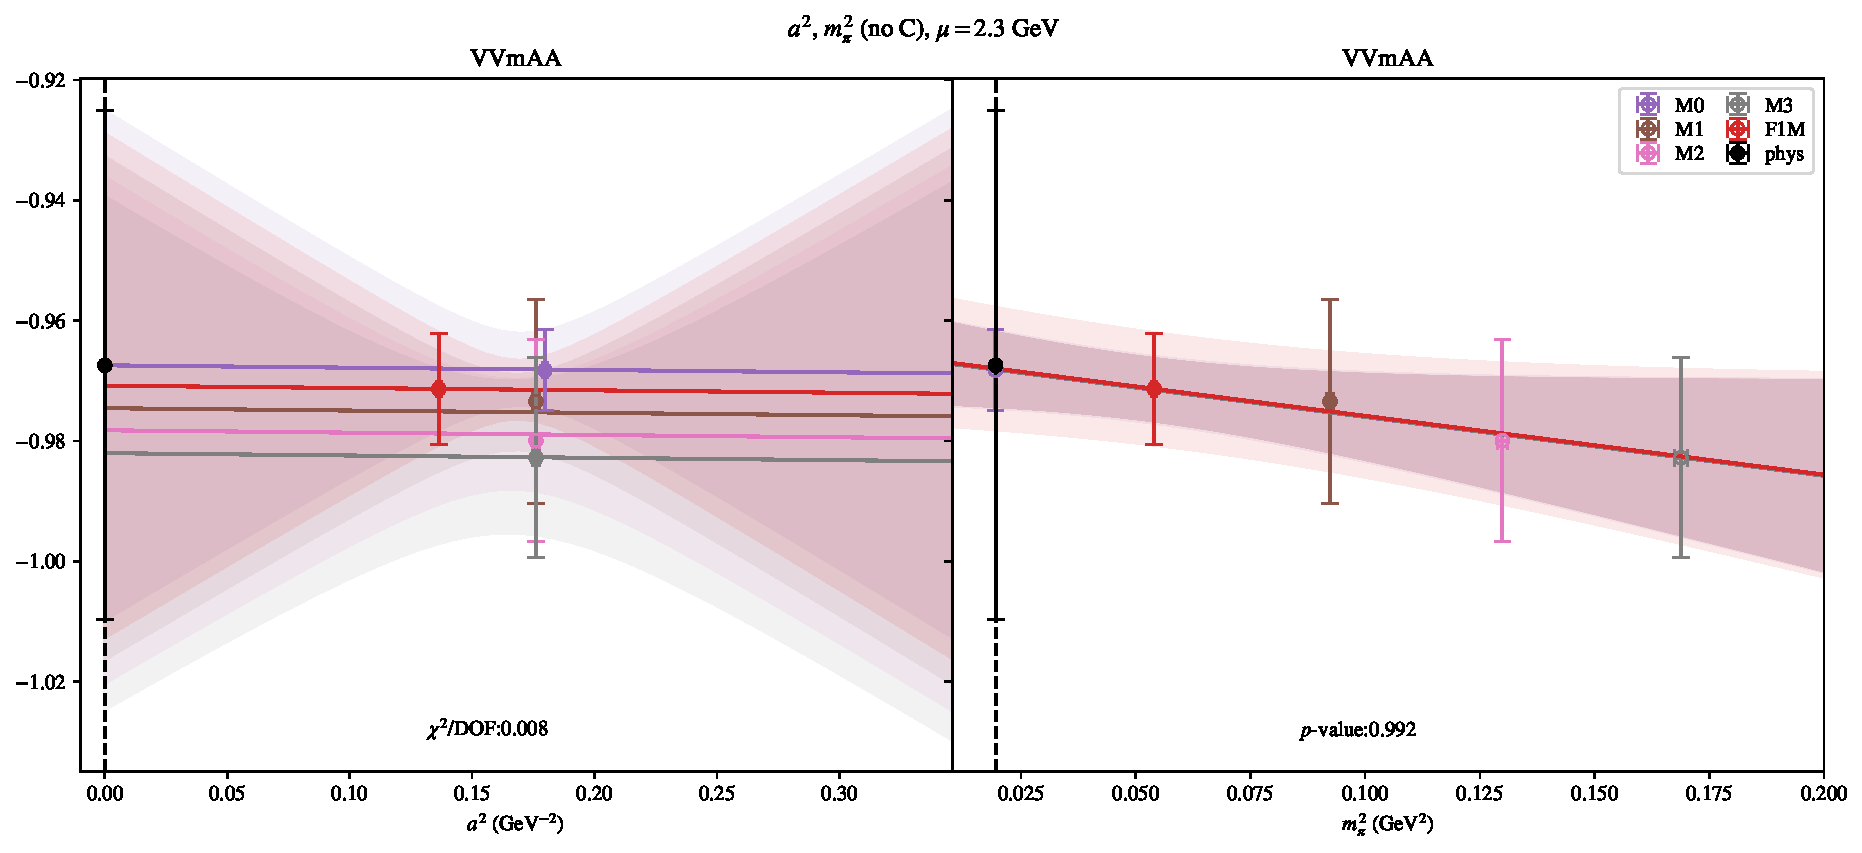
\includepdf[link, pages=-]{VVmAA/NPR/bag_a2m2noC_23.pdf}
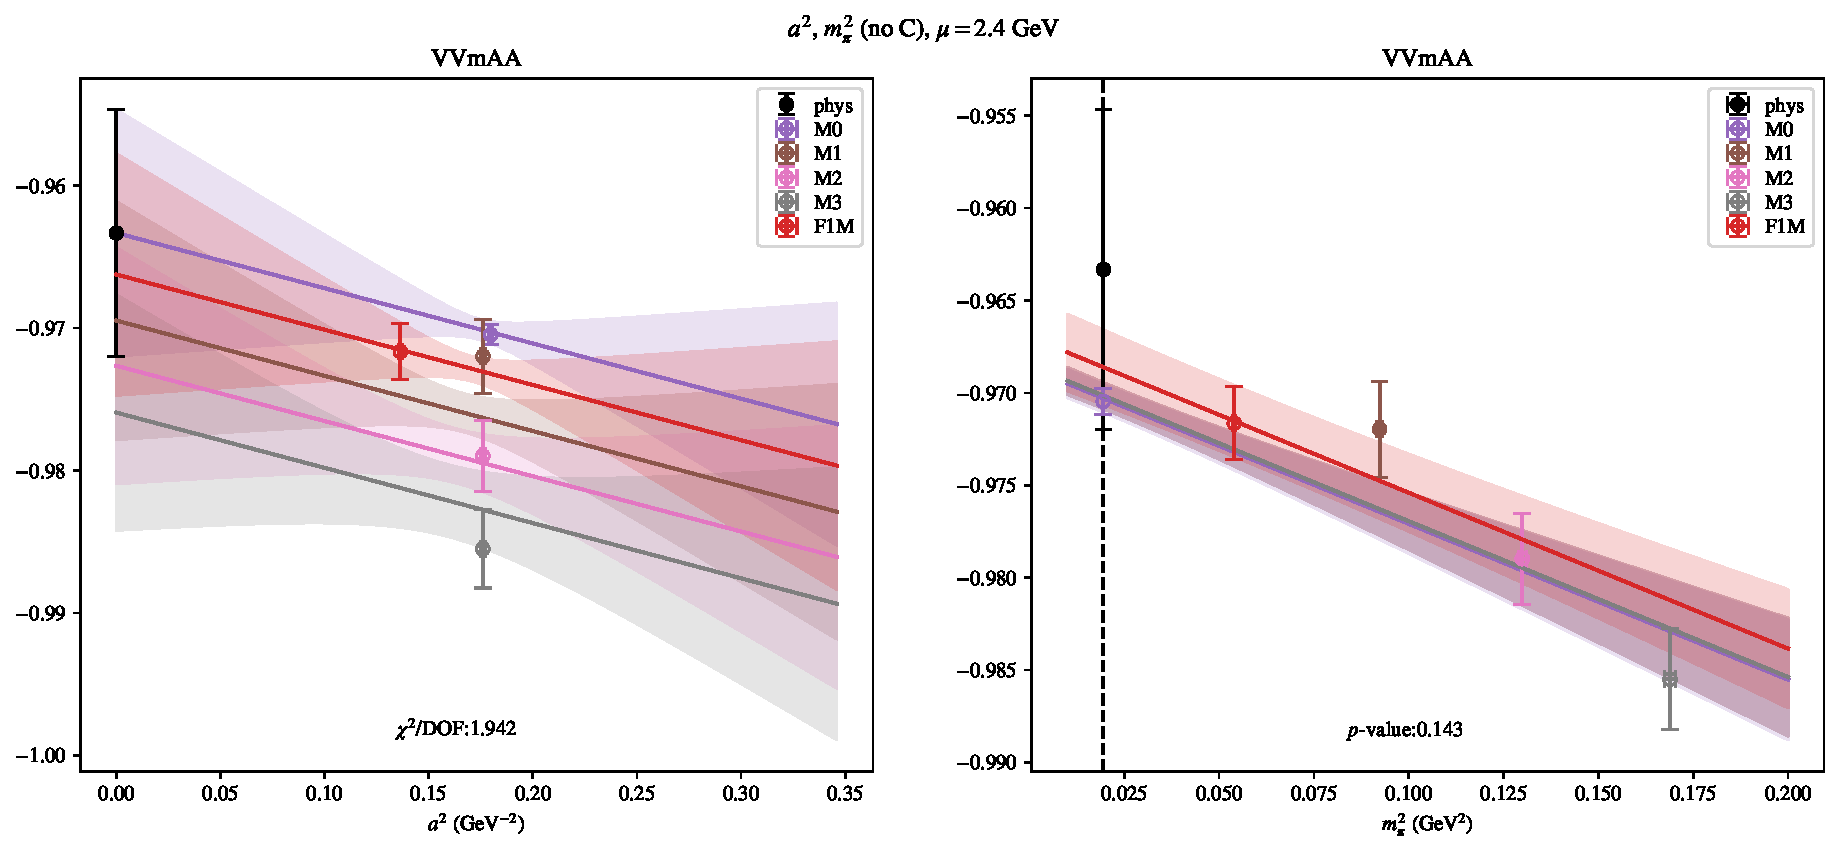
\includepdf[link, pages=-]{VVmAA/NPR/bag_a2m2noC_24.pdf}
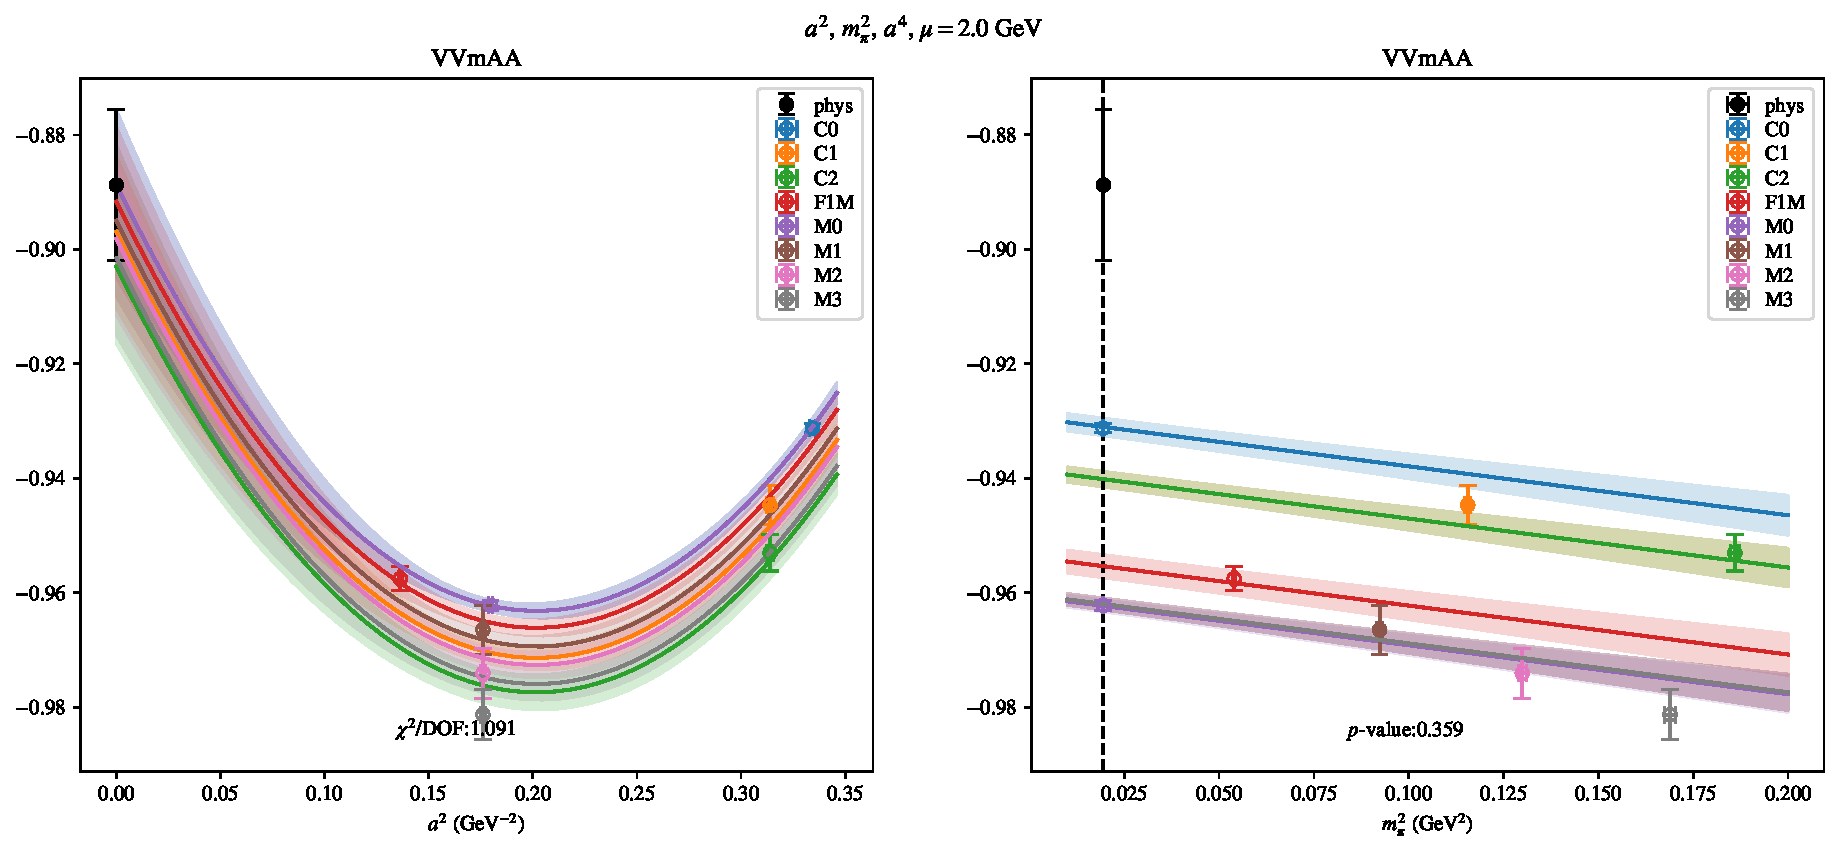
\includepdf[link, pages=-]{VVmAA/NPR/bag_a2a4m2_20.pdf}
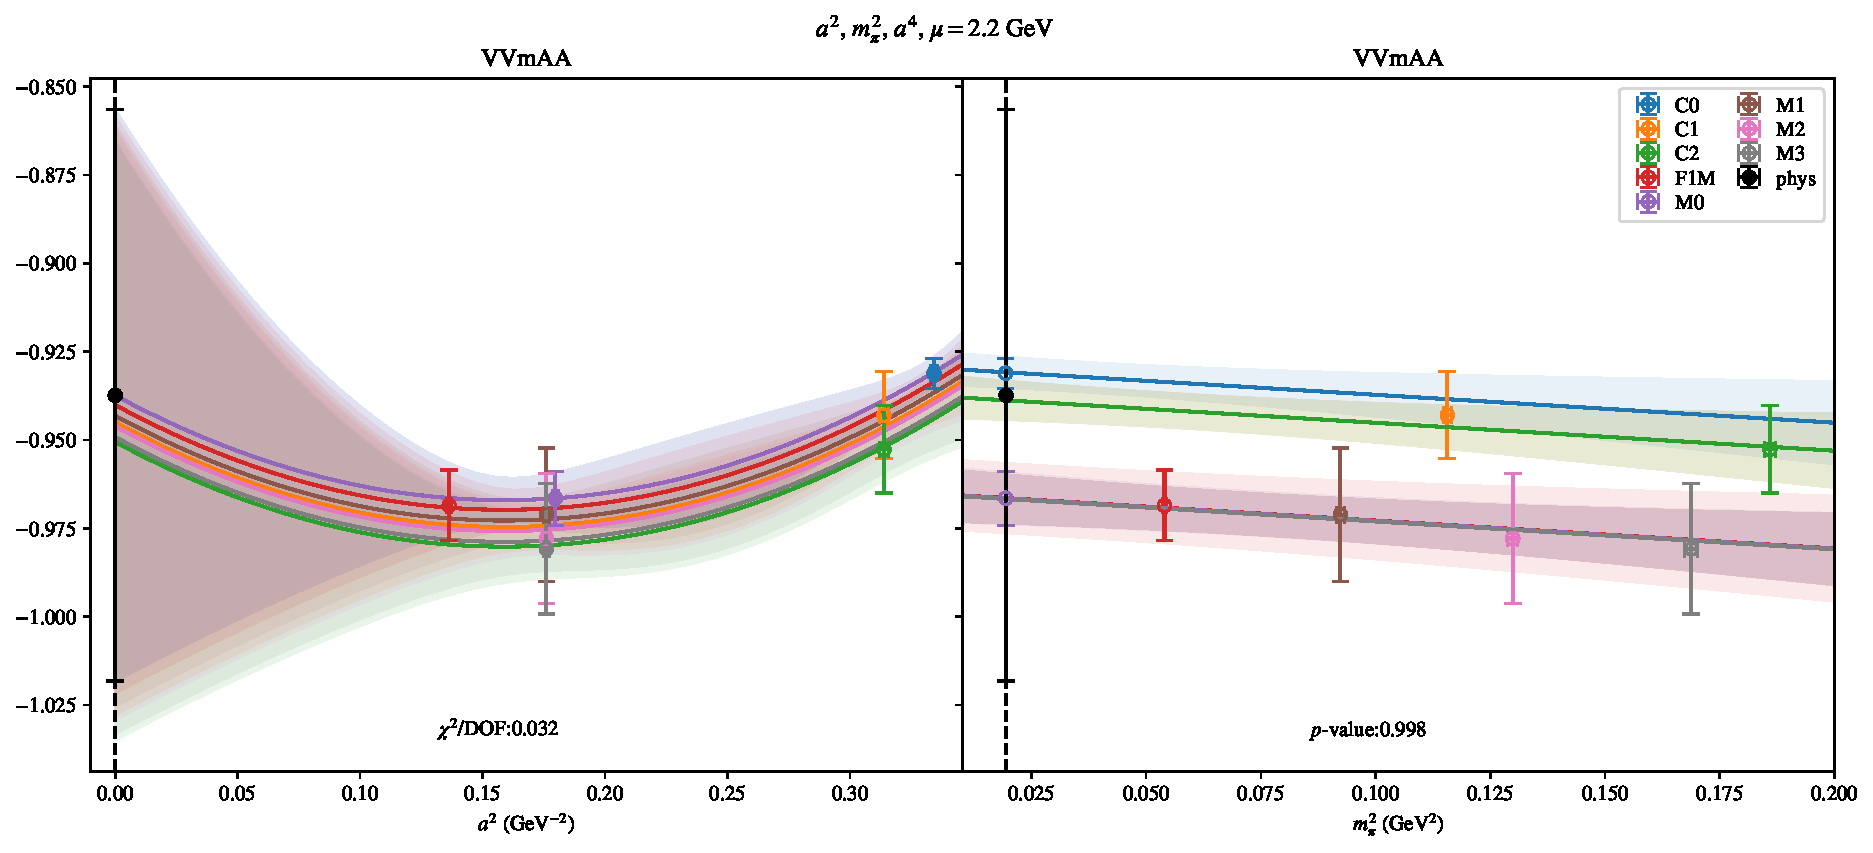
\includepdf[link, pages=-]{VVmAA/NPR/bag_a2a4m2_22.pdf}
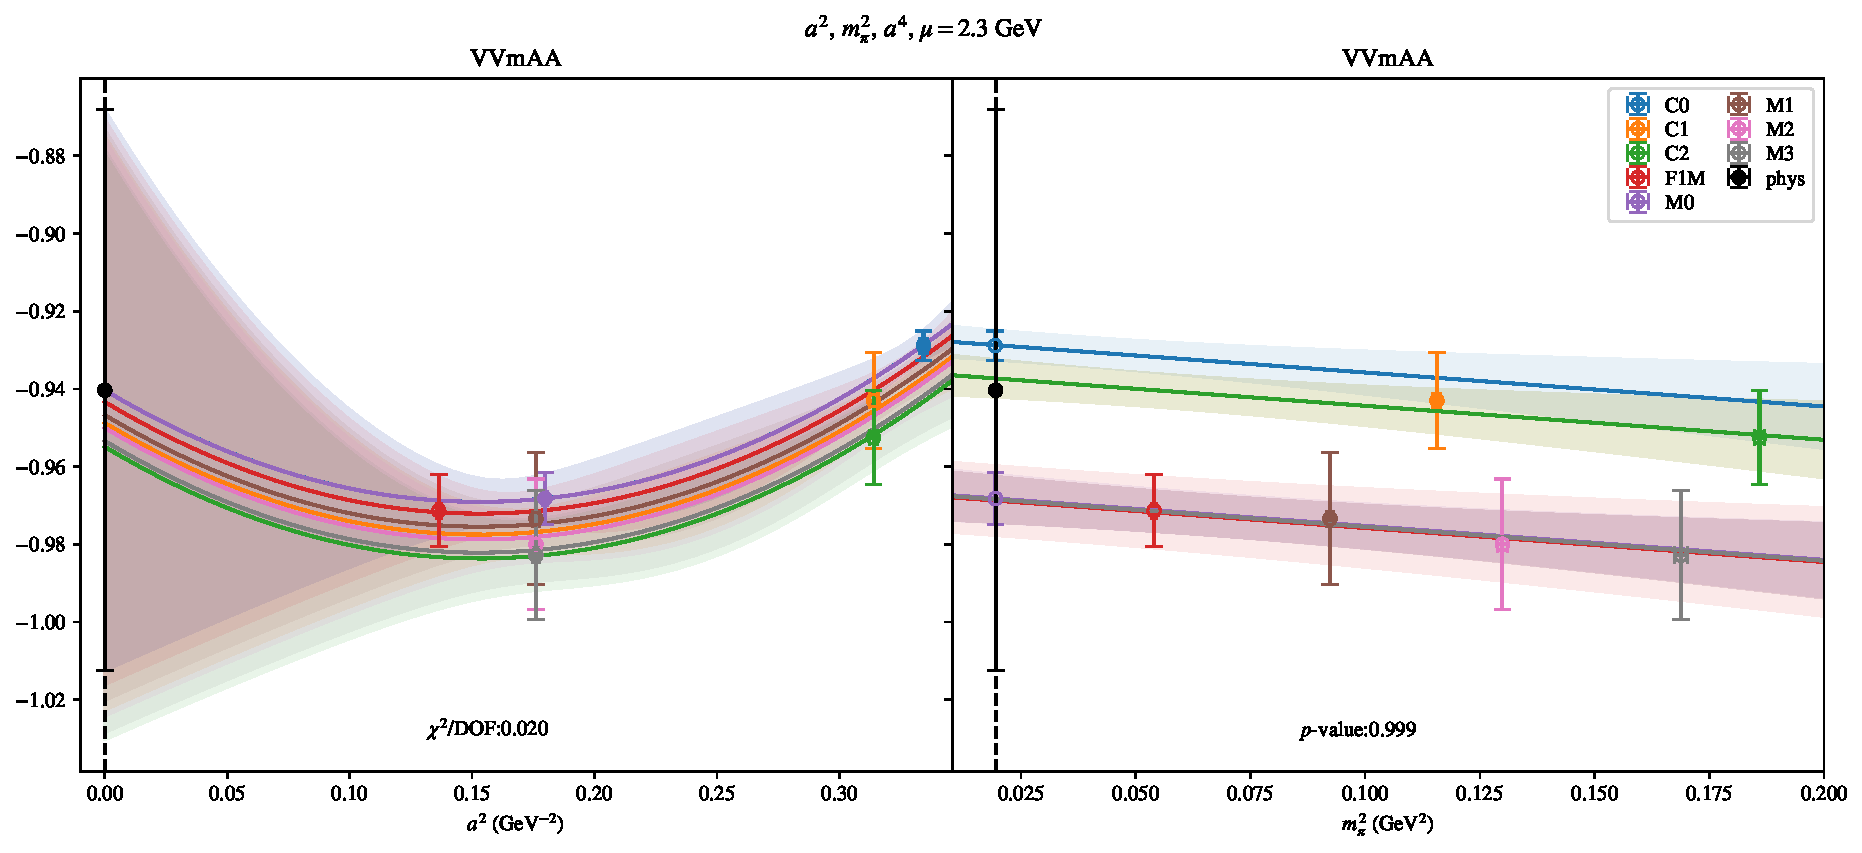
\includepdf[link, pages=-]{VVmAA/NPR/bag_a2a4m2_23.pdf}
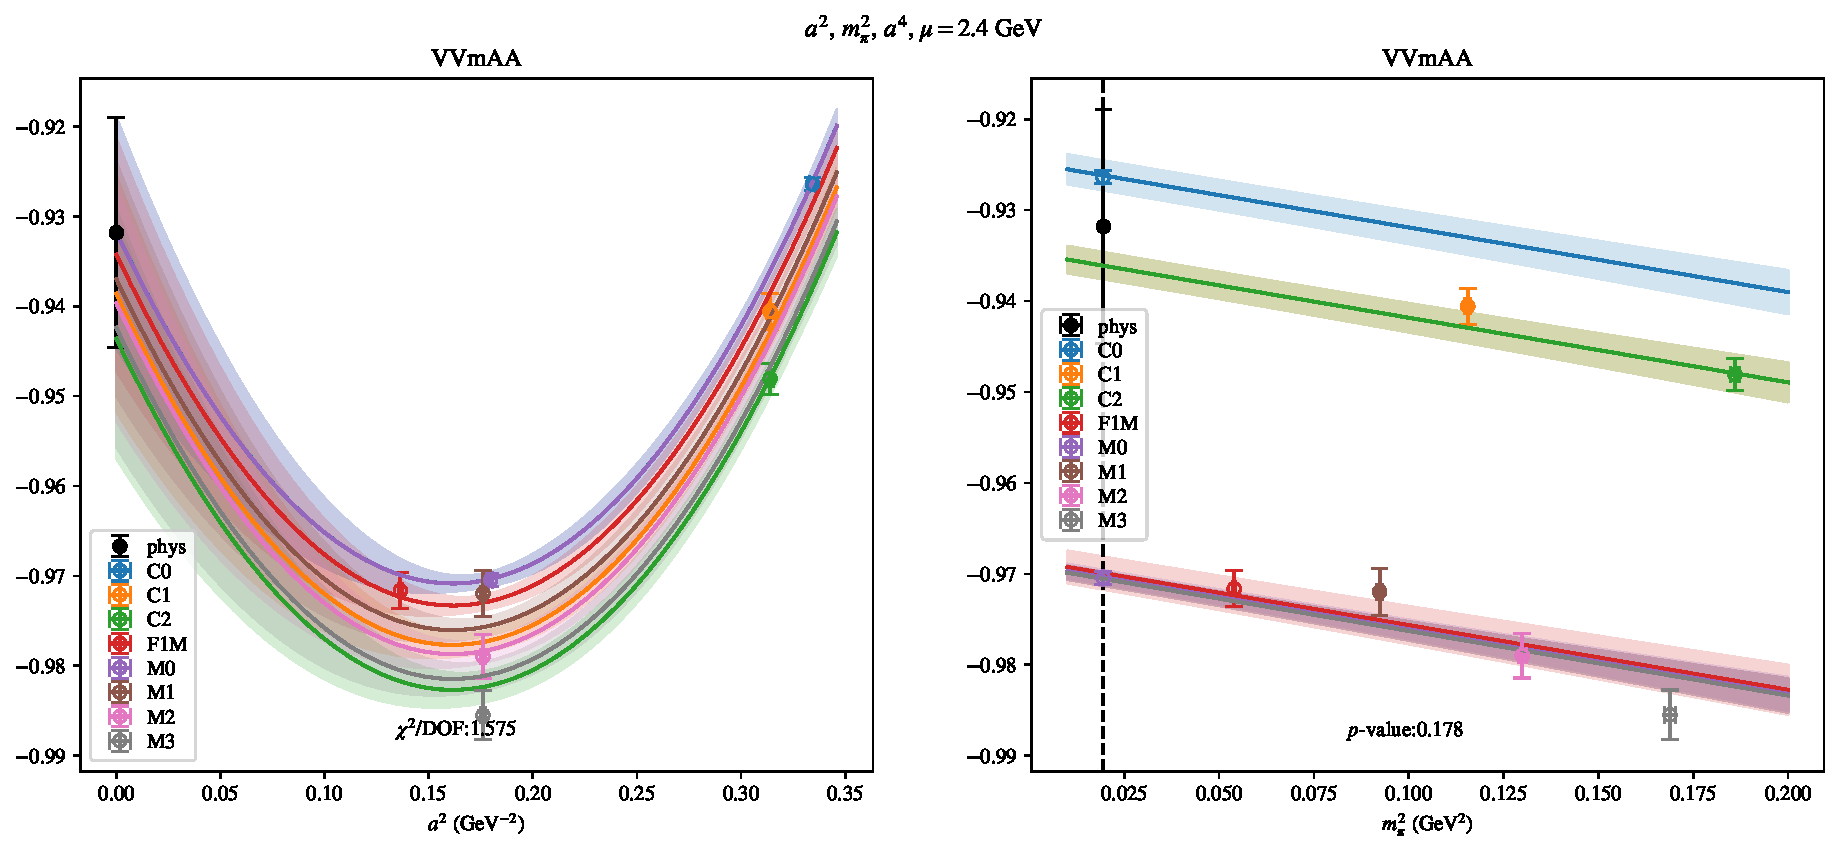
\includepdf[link, pages=-]{VVmAA/NPR/bag_a2a4m2_24.pdf}
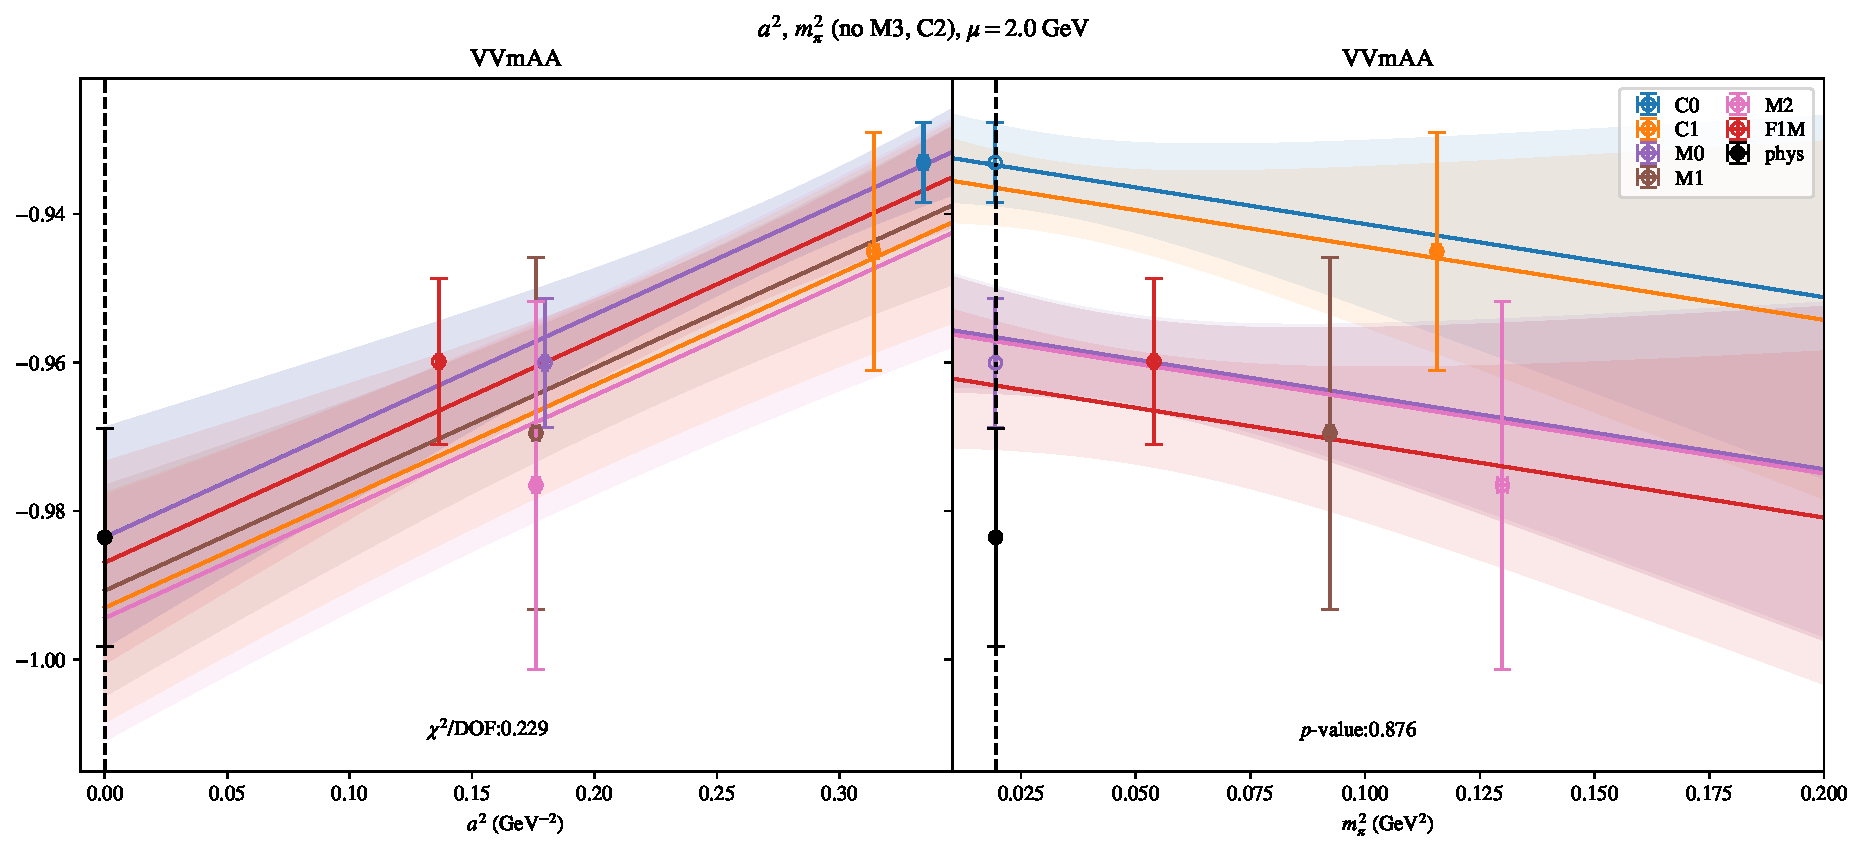
\includepdf[link, pages=-]{VVmAA/NPR/bag_a2m2mcut_20.pdf}
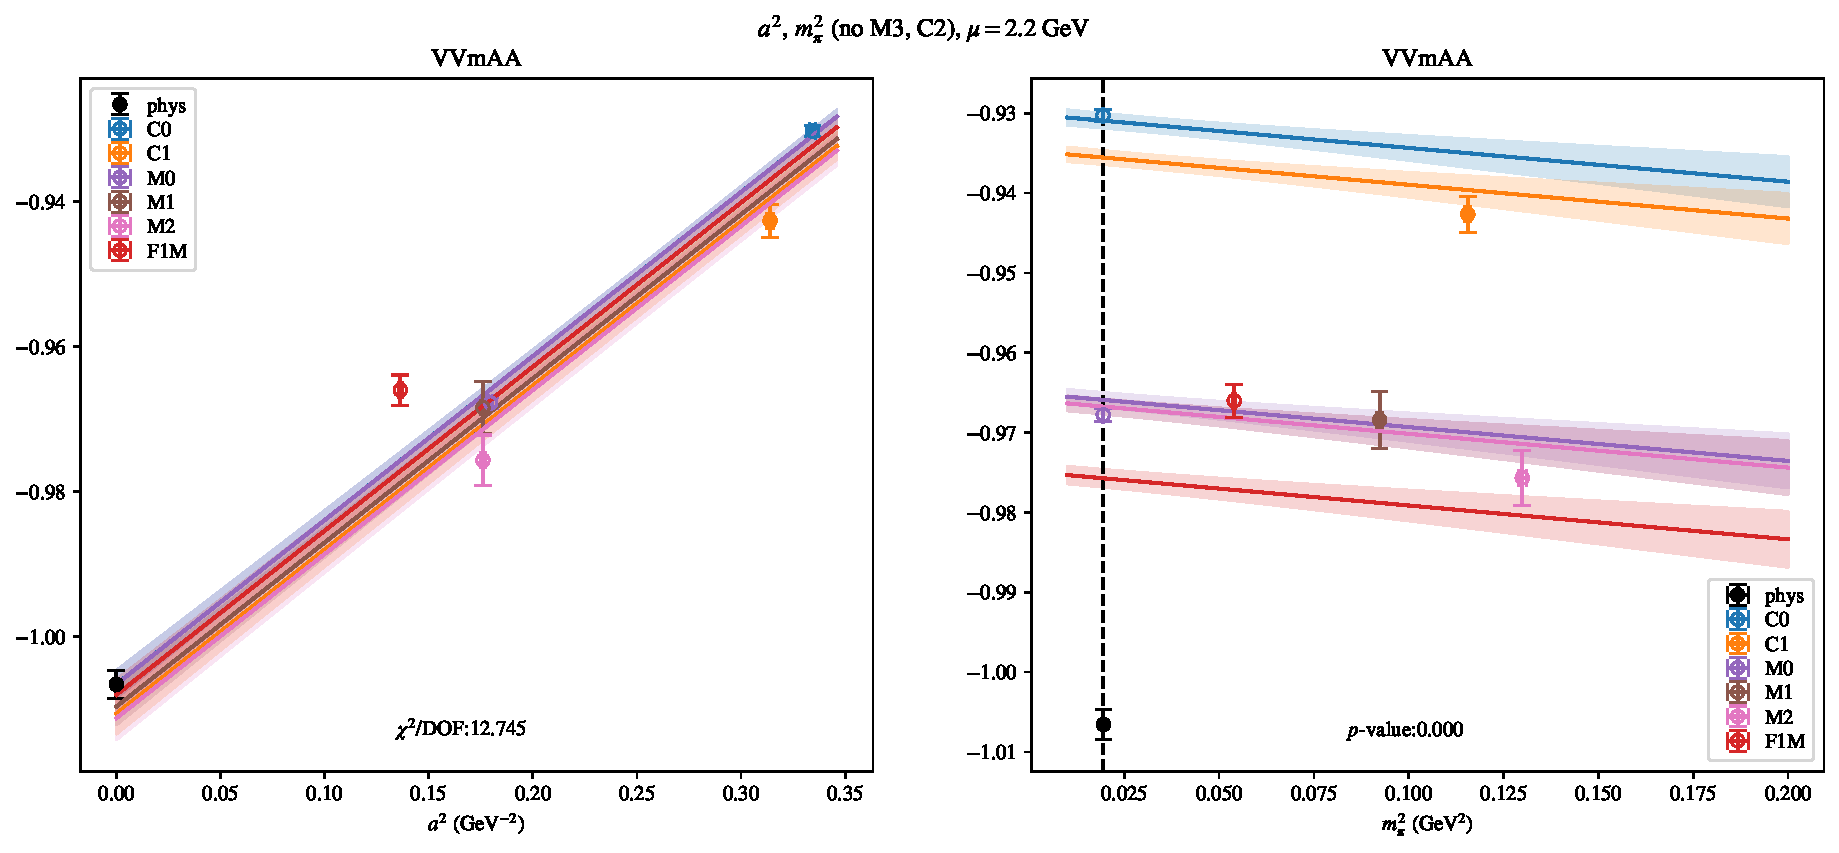
\includepdf[link, pages=-]{VVmAA/NPR/bag_a2m2mcut_22.pdf}
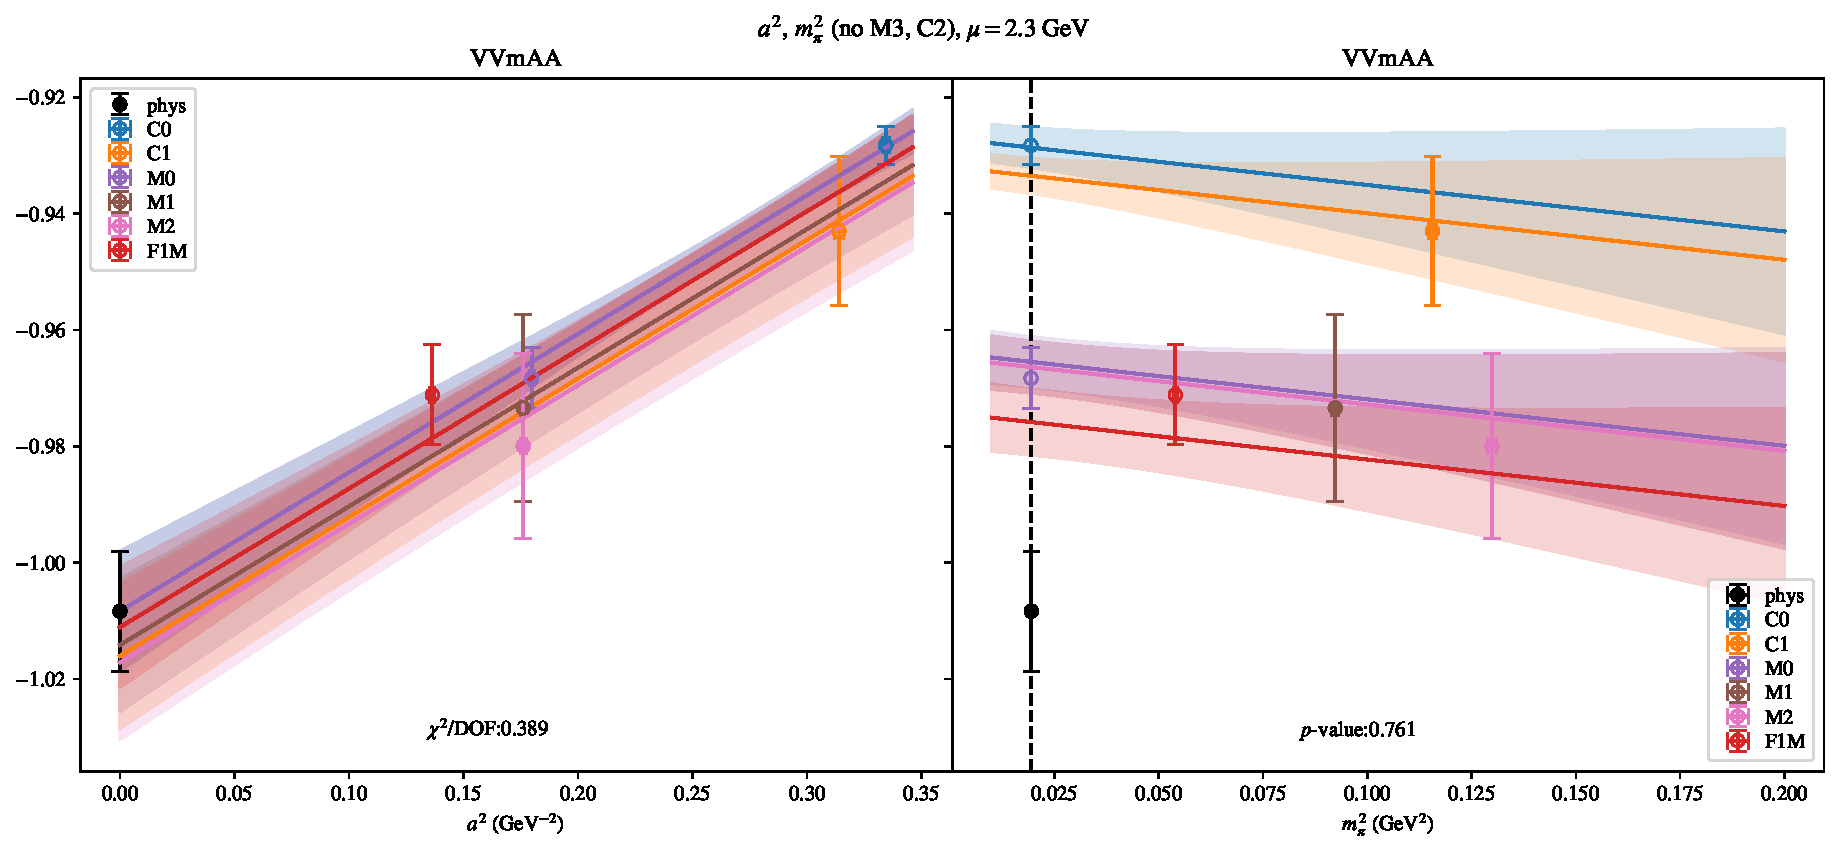
\includepdf[link, pages=-]{VVmAA/NPR/bag_a2m2mcut_23.pdf}
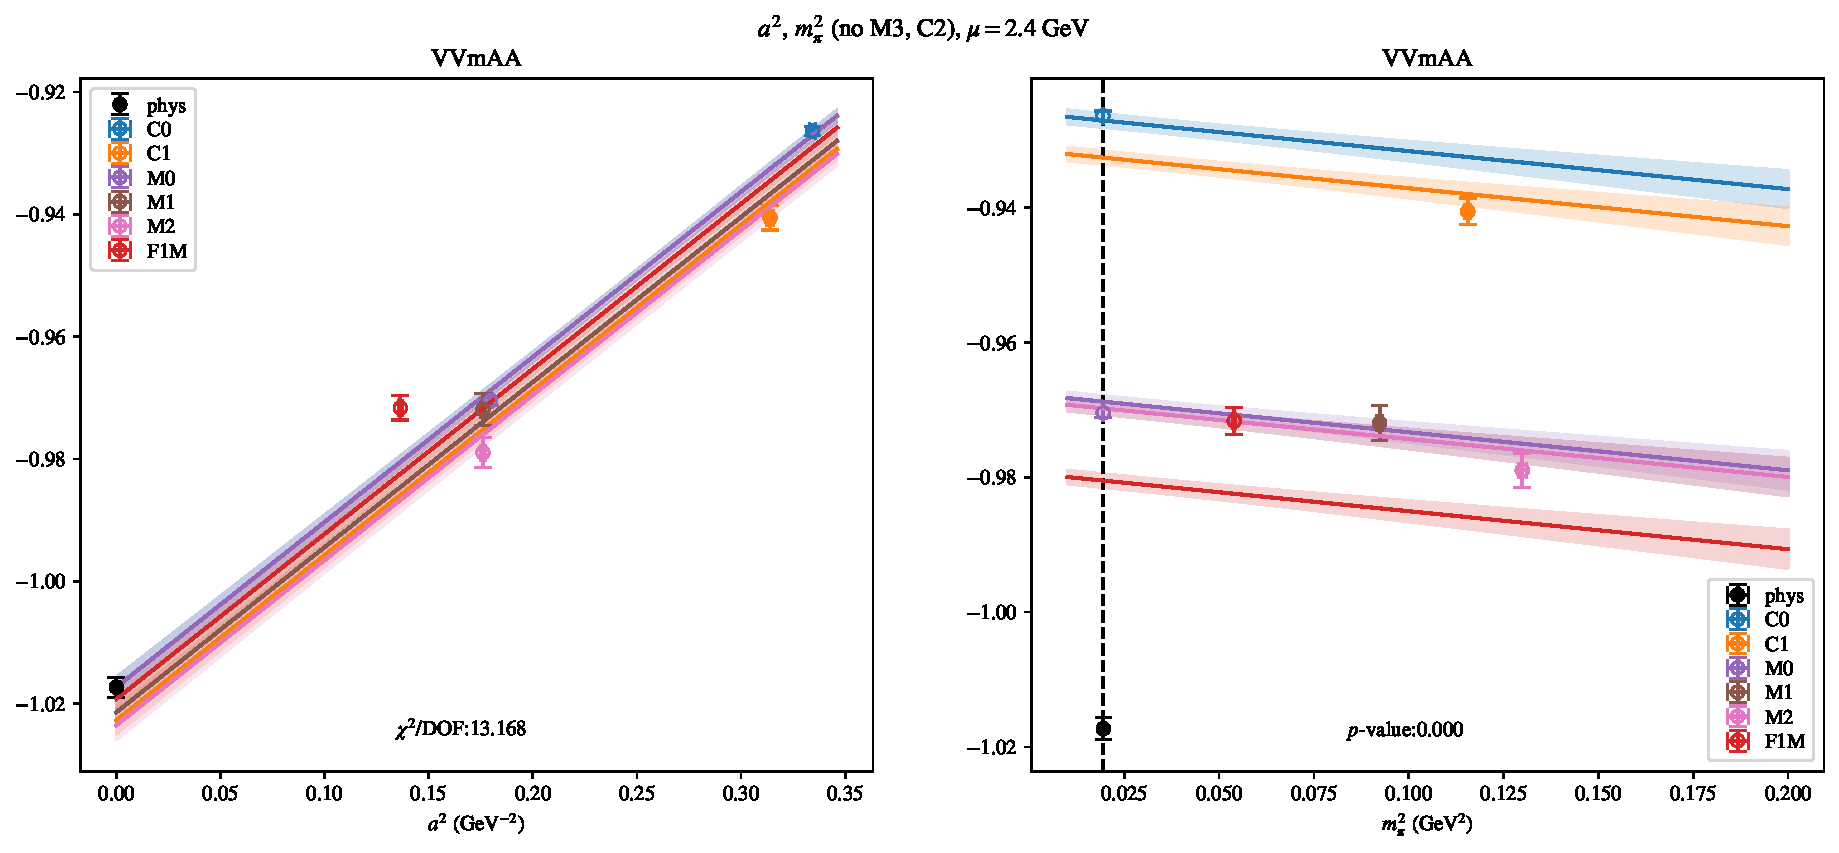
\includepdf[link, pages=-]{VVmAA/NPR/bag_a2m2mcut_24.pdf}
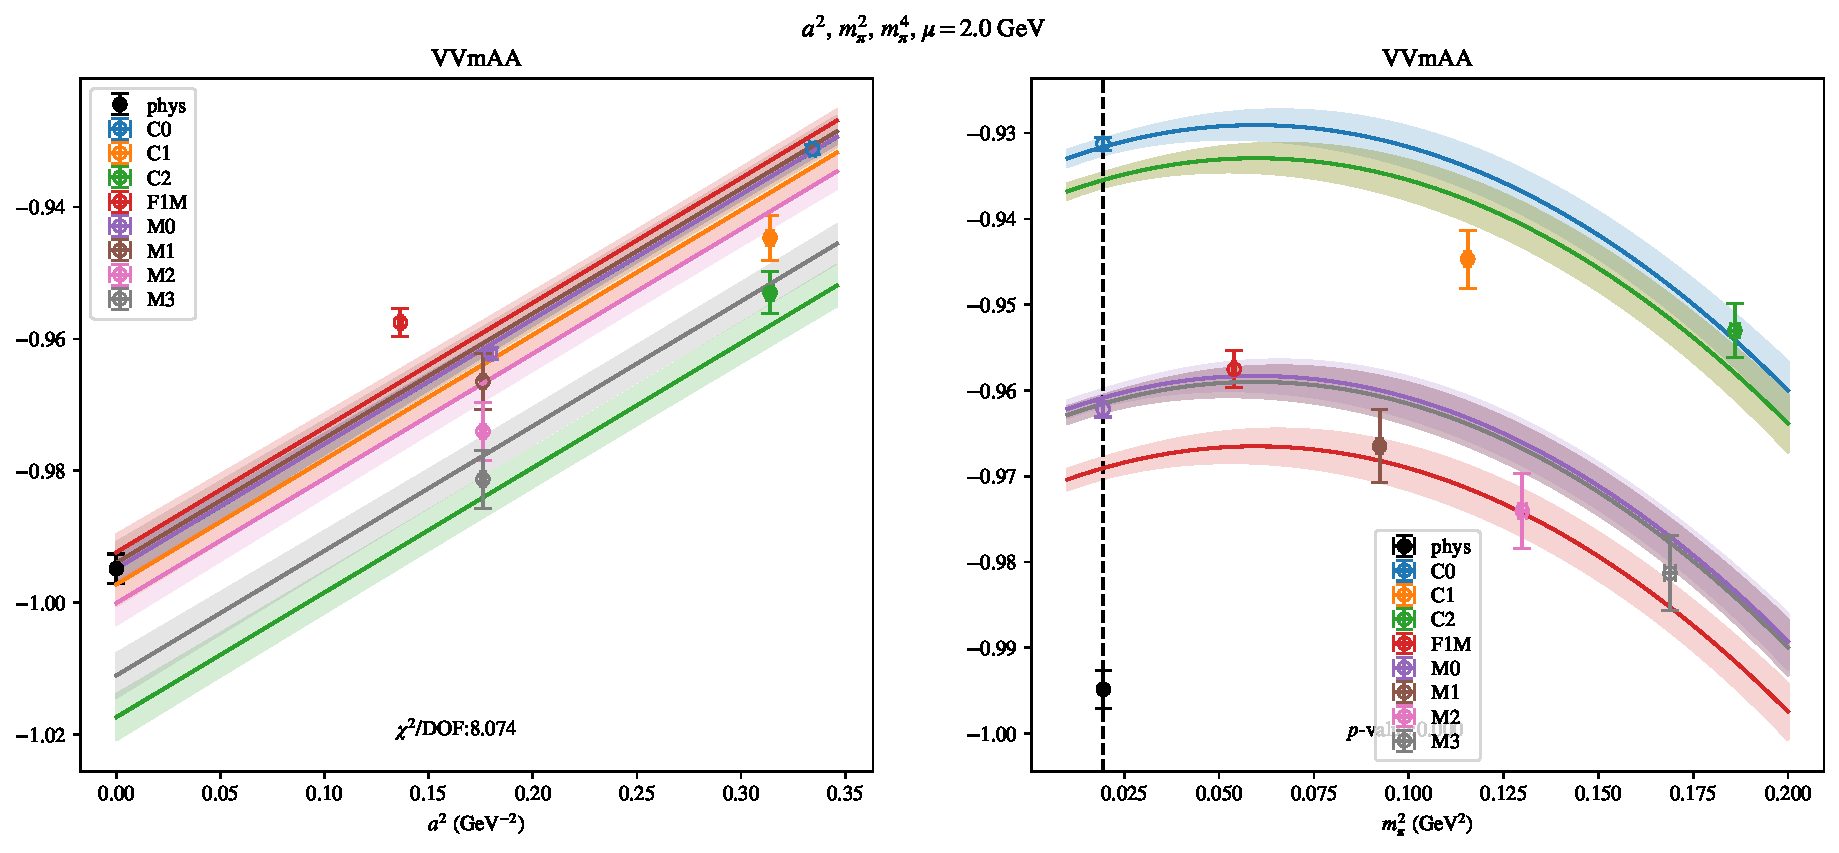
\includepdf[link, pages=-]{VVmAA/NPR/bag_a2m2m4_20.pdf}
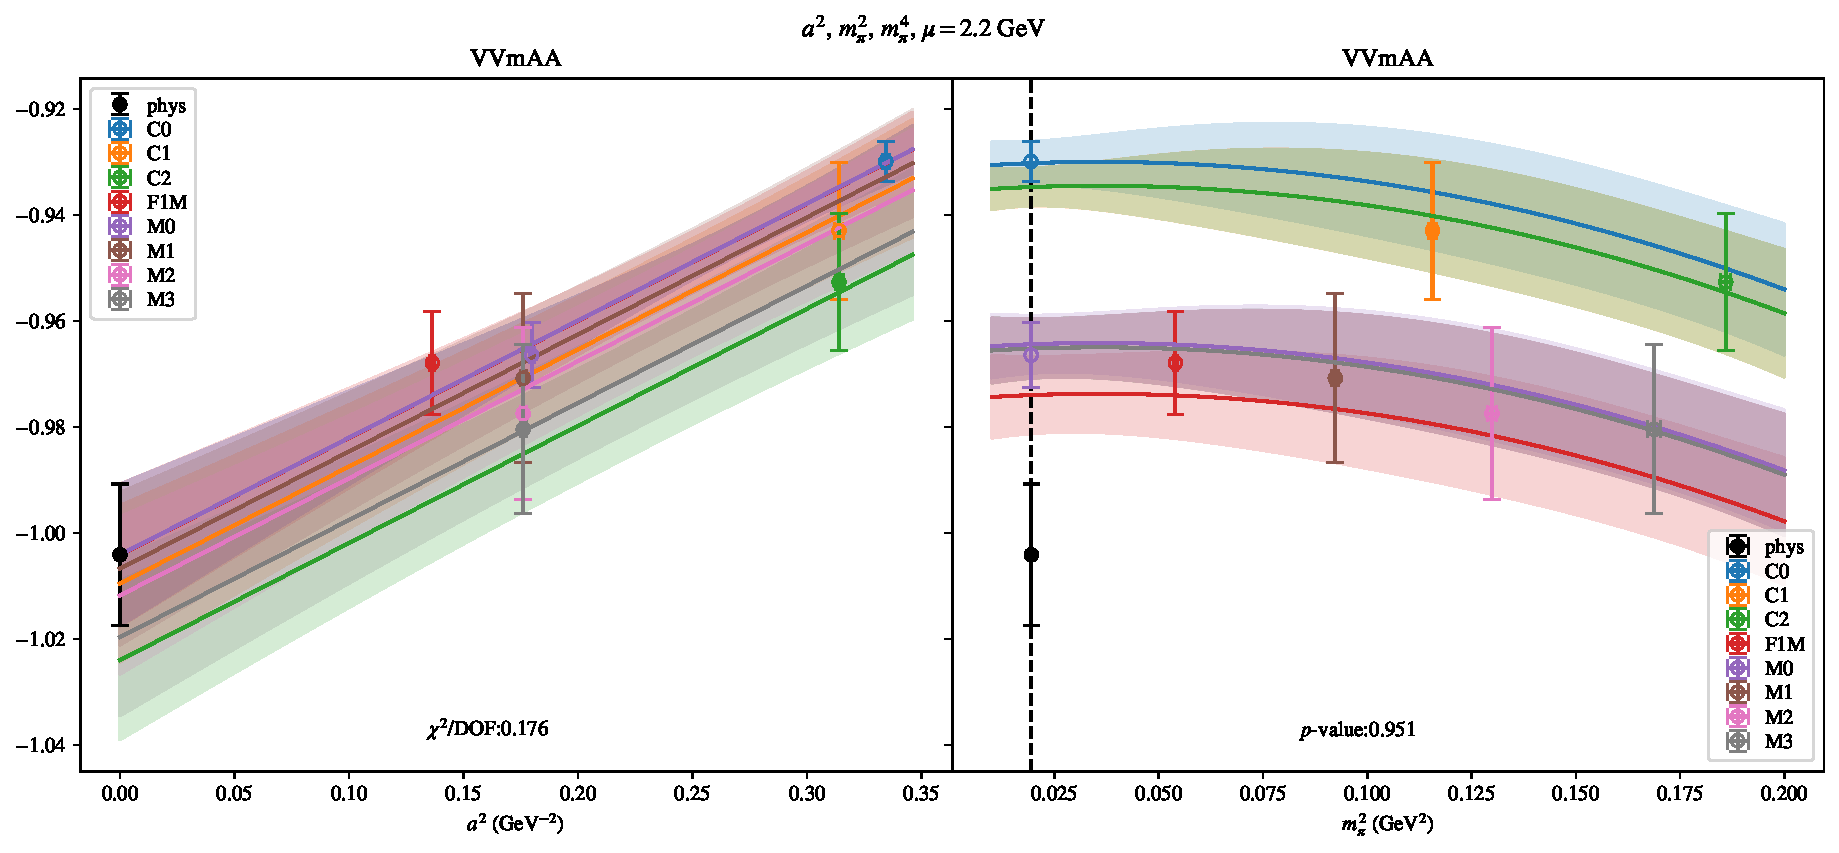
\includepdf[link, pages=-]{VVmAA/NPR/bag_a2m2m4_22.pdf}
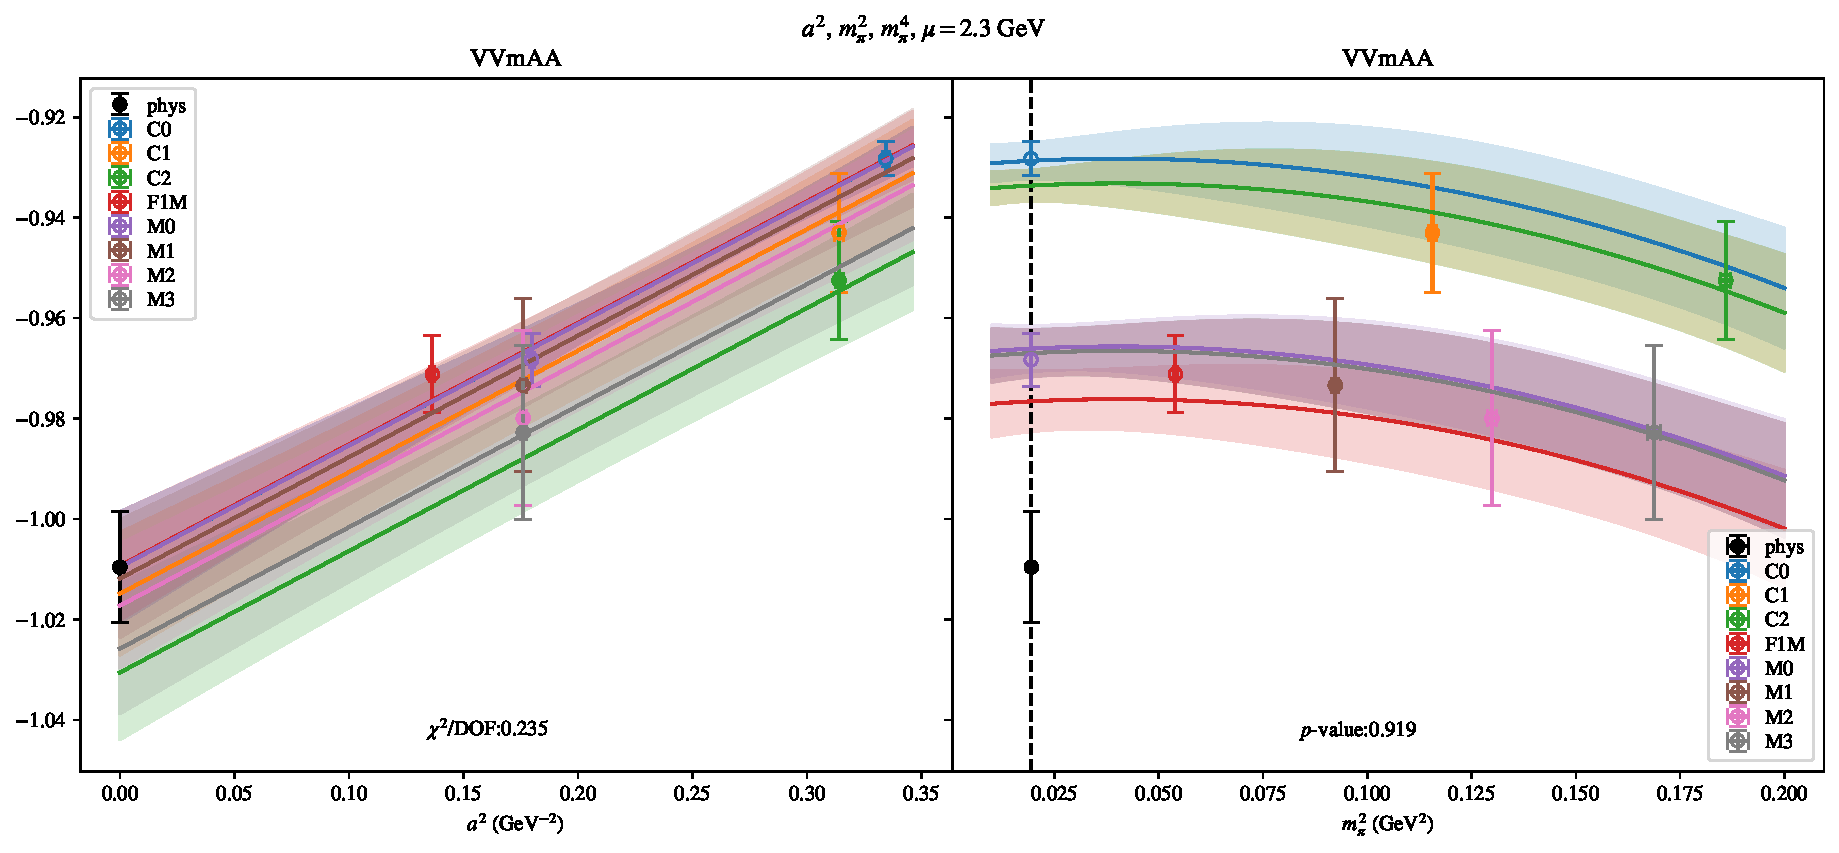
\includepdf[link, pages=-]{VVmAA/NPR/bag_a2m2m4_23.pdf}
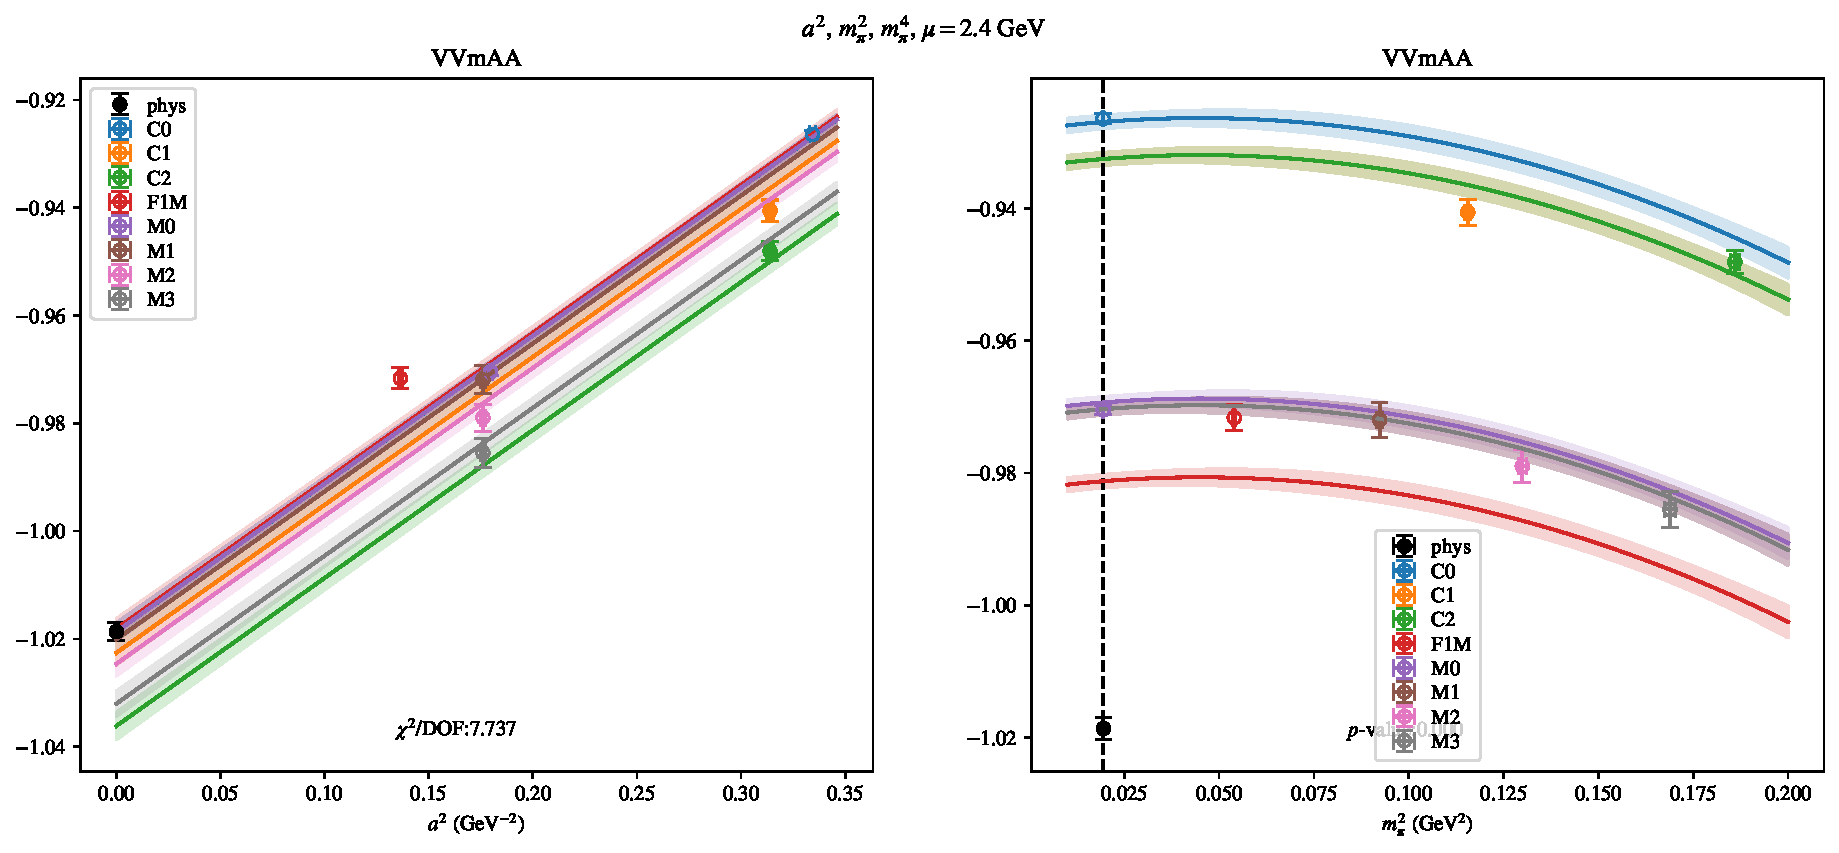
\includepdf[link, pages=-]{VVmAA/NPR/bag_a2m2m4_24.pdf}
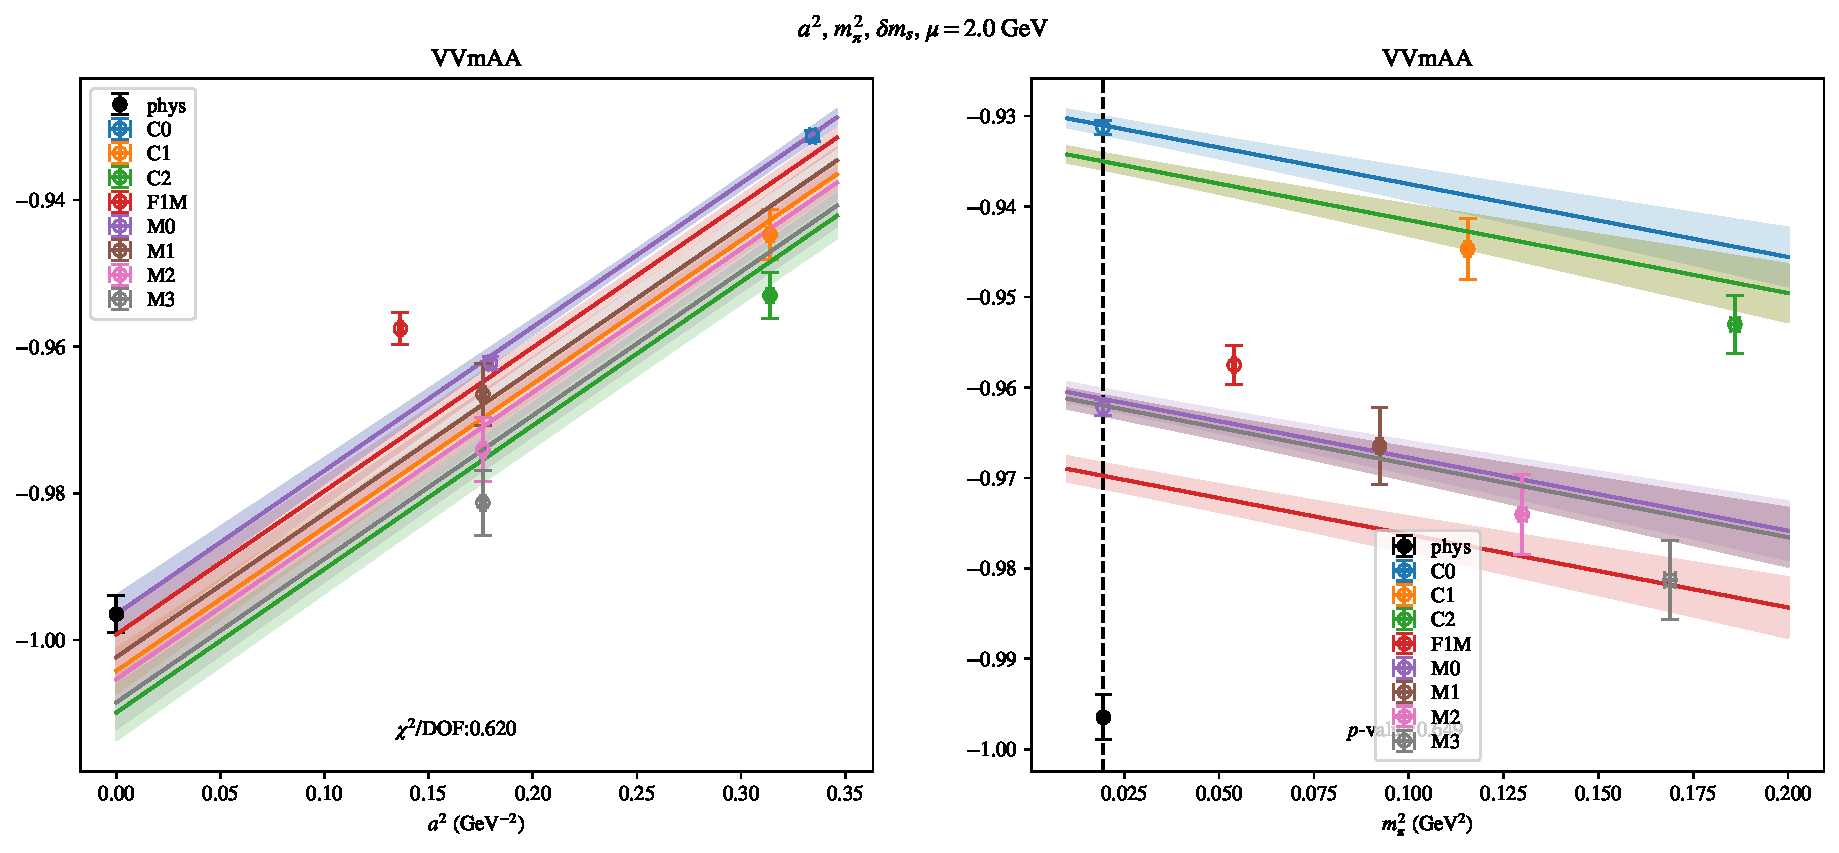
\includepdf[link, pages=-]{VVmAA/NPR/bag_a2m2delm_20.pdf}
\includepdf[link, pages=-]{VVmAA/NPR/bag_a2m2delm_22.pdf}
\includepdf[link, pages=-]{VVmAA/NPR/bag_a2m2delm_23.pdf}
\includepdf[link, pages=-]{VVmAA/NPR/bag_a2m2delm_24.pdf}
\clearpage
\section{$\mathcal{B}_3$}
\begin{table}[h!]
\begin{center}
\begin{tabular}{|c|c|c|c|c|c|c|}
\hline
$\mu$ (GeV) & $a^2$, $m_\pi^2$& $a^2$, $m_\pi^2$ (no C)& $a^2$, $m_\pi^2$, $a^4$& $a^2$, $m_\pi^2$ (no M3, C2)& $a^2$, $m_\pi^2$, $m_\pi^4$& $a^2$, $m_\pi^2$, $\delta m_s$\\
\hline
2.0& \hyperlink{SSmPP/NPR/bag_a2m2_20.pdf.1}{\textbf{1.8001(27)}: 16.056 (0.0)} & \hyperlink{SSmPP/NPR/bag_a2m2noC_20.pdf.1}{\textbf{1.692(12)}: 0.645 (0.524)} & \hyperlink{SSmPP/NPR/bag_a2a4m2_20.pdf.1}{\textbf{1.622(19)}: 1.037 (0.386)} & \hyperlink{SSmPP/NPR/bag_a2m2mcut_20.pdf.1}{\textbf{1.8013(27)}: 25.255 (0.0)} & \hyperlink{SSmPP/NPR/bag_a2m2m4_20.pdf.1}{\textbf{1.8052(28)}: 15.441 (0.0)} & \hyperlink{SSmPP/NPR/bag_a2m2delm_20.pdf.1}{\textbf{1.8092(28)}: 1.286 (0.273)}\\
2.2& \hyperlink{SSmPP/NPR/bag_a2m2_22.pdf.1}{\textbf{1.8057(26)}: 15.0 (0.0)} & \hyperlink{SSmPP/NPR/bag_a2m2noC_22.pdf.1}{\textbf{1.705(12)}: 1.351 (0.259)} & \hyperlink{SSmPP/NPR/bag_a2a4m2_22.pdf.1}{\textbf{1.639(19)}: 1.491 (0.202)} & \hyperlink{SSmPP/NPR/bag_a2m2mcut_22.pdf.1}{\textbf{1.8072(27)}: 22.444 (0.0)} & \hyperlink{SSmPP/NPR/bag_a2m2m4_22.pdf.1}{\textbf{1.8110(27)}: 13.454 (0.0)} & \hyperlink{SSmPP/NPR/bag_a2m2delm_22.pdf.1}{\textbf{1.8141(28)}: 2.2 (0.066)}\\
2.3& \hyperlink{SSmPP/NPR/bag_a2m2_23.pdf.1}{\textbf{1.8080(25)}: 14.151 (0.0)} & \hyperlink{SSmPP/NPR/bag_a2m2noC_23.pdf.1}{\textbf{1.710(12)}: 1.486 (0.226)} & \hyperlink{SSmPP/NPR/bag_a2a4m2_23.pdf.1}{\textbf{1.645(19)}: 1.376 (0.239)} & \hyperlink{SSmPP/NPR/bag_a2m2mcut_23.pdf.1}{\textbf{1.8093(27)}: 21.469 (0.0)} & \hyperlink{SSmPP/NPR/bag_a2m2m4_23.pdf.1}{\textbf{1.8130(27)}: 13.142 (0.0)} & \hyperlink{SSmPP/NPR/bag_a2m2delm_23.pdf.1}{\textbf{1.8158(27)}: 2.182 (0.068)}\\
2.4& \hyperlink{SSmPP/NPR/bag_a2m2_24.pdf.1}{\textbf{1.8094(25)}: 13.238 (0.0)} & \hyperlink{SSmPP/NPR/bag_a2m2noC_24.pdf.1}{\textbf{1.715(12)}: 1.507 (0.222)} & \hyperlink{SSmPP/NPR/bag_a2a4m2_24.pdf.1}{\textbf{1.652(19)}: 1.347 (0.25)} & \hyperlink{SSmPP/NPR/bag_a2m2mcut_24.pdf.1}{\textbf{1.8106(27)}: 20.226 (0.0)} & \hyperlink{SSmPP/NPR/bag_a2m2m4_24.pdf.1}{\textbf{1.8143(27)}: 12.521 (0.0)} & \hyperlink{SSmPP/NPR/bag_a2m2delm_24.pdf.1}{\textbf{1.8168(26)}: 2.143 (0.073)}\\
\hline
\end{tabular}
\caption{Physical point value from chiral and continuum extrapolation at renormalisation scale $\mu$. Entries are \textbf{value(error)}: $\chi^2/\text{DOF}$ ($p$-value).}
\end{center}
\end{table}
\begin{table}[h!]
\begin{center}
\begin{tabular}{|c c|c|c|c|c|c|c|}
\hline
$\mu$ (GeV) &  & $a^2$, $m_\pi^2$& $a^2$, $m_\pi^2$ (no C)& $a^2$, $m_\pi^2$, $a^4$& $a^2$, $m_\pi^2$ (no M3, C2)& $a^2$, $m_\pi^2$, $m_\pi^4$& $a^2$, $m_\pi^2$, $\delta m_s$\\
\hline
\multirow{3}{0.5in}{2.0} & $\alpha$ & 0.128(10)& 0.759(72)& 1.73(17)& 0.124(10)& 0.111(10)& 0.095(10)\\
 & $\beta$ & -0.00198(23)& -0.00199(42)& -0.00254(24)& -0.00274(44)& -0.0074(12)& -0.00256(24)\\
 & $\gamma$ &  &  & -3.22(35)&  & 0.00049(11)& 0.0278(31)\\
\hline
\multirow{3}{0.5in}{2.2} & $\alpha$ & 0.1377(99)& 0.728(71)& 1.64(17)& 0.134(10)& 0.121(10)& 0.107(10)\\
 & $\beta$ & -0.00136(21)& -0.00152(39)& -0.00191(22)& -0.00234(42)& -0.0069(11)& -0.00193(22)\\
 & $\gamma$ &  &  & -3.02(35)&  & 0.00049(10)& 0.0257(31)\\
\hline
\multirow{3}{0.5in}{2.3} & $\alpha$ & 0.1402(98)& 0.713(71)& 1.60(17)& 0.137(10)& 0.124(10)& 0.112(10)\\
 & $\beta$ & -0.00127(21)& -0.00143(36)& -0.00181(21)& -0.00212(41)& -0.0063(11)& -0.00183(21)\\
 & $\gamma$ &  &  & -2.94(35)&  & 0.00044(10)& 0.0248(31)\\
\hline
\multirow{3}{0.5in}{2.4} & $\alpha$ & 0.1432(97)& 0.697(71)& 1.56(17)& 0.140(10)& 0.127(10)& 0.116(10)\\
 & $\beta$ & -0.00119(20)& -0.00135(35)& -0.00172(21)& -0.00194(39)& -0.0058(11)& -0.00174(21)\\
 & $\gamma$ &  &  & -2.84(35)&  & 0.000410(99)& 0.0239(31)\\
\hline
\end{tabular}
\caption{Fit values of coefficients in $Q = Q_{phys} + \mathbf{\alpha} a^2 + \mathbf{\beta}\left(\frac{m_\pi^2}{f_\pi^2}-\frac{m_{\pi,PDG}^2}{f_\pi^2}\right) + \gamma(\ldots)$}
\end{center}
\end{table}
\includepdf[link, pages=-]{SSmPP/NPR/bag_a2m2_20.pdf}
\includepdf[link, pages=-]{SSmPP/NPR/bag_a2m2_22.pdf}
\includepdf[link, pages=-]{SSmPP/NPR/bag_a2m2_23.pdf}
\includepdf[link, pages=-]{SSmPP/NPR/bag_a2m2_24.pdf}
\includepdf[link, pages=-]{SSmPP/NPR/bag_a2m2noC_20.pdf}
\includepdf[link, pages=-]{SSmPP/NPR/bag_a2m2noC_22.pdf}
\includepdf[link, pages=-]{SSmPP/NPR/bag_a2m2noC_23.pdf}
\includepdf[link, pages=-]{SSmPP/NPR/bag_a2m2noC_24.pdf}
\includepdf[link, pages=-]{SSmPP/NPR/bag_a2a4m2_20.pdf}
\includepdf[link, pages=-]{SSmPP/NPR/bag_a2a4m2_22.pdf}
\includepdf[link, pages=-]{SSmPP/NPR/bag_a2a4m2_23.pdf}
\includepdf[link, pages=-]{SSmPP/NPR/bag_a2a4m2_24.pdf}
\includepdf[link, pages=-]{SSmPP/NPR/bag_a2m2mcut_20.pdf}
\includepdf[link, pages=-]{SSmPP/NPR/bag_a2m2mcut_22.pdf}
\includepdf[link, pages=-]{SSmPP/NPR/bag_a2m2mcut_23.pdf}
\includepdf[link, pages=-]{SSmPP/NPR/bag_a2m2mcut_24.pdf}
\includepdf[link, pages=-]{SSmPP/NPR/bag_a2m2m4_20.pdf}
\includepdf[link, pages=-]{SSmPP/NPR/bag_a2m2m4_22.pdf}
\includepdf[link, pages=-]{SSmPP/NPR/bag_a2m2m4_23.pdf}
\includepdf[link, pages=-]{SSmPP/NPR/bag_a2m2m4_24.pdf}
\includepdf[link, pages=-]{SSmPP/NPR/bag_a2m2delm_20.pdf}
\includepdf[link, pages=-]{SSmPP/NPR/bag_a2m2delm_22.pdf}
\includepdf[link, pages=-]{SSmPP/NPR/bag_a2m2delm_23.pdf}
\includepdf[link, pages=-]{SSmPP/NPR/bag_a2m2delm_24.pdf}
\clearpage
\section{$\mathcal{B}_4$}
\begin{table}[h!]
\begin{center}
\begin{tabular}{|c|c|c|c|c|c|c|}
\hline
$\mu$ (GeV) & $a^2$, $m_\pi^2$& $a^2$, $m_\pi^2$ (no C)& $a^2$, $m_\pi^2$, $a^4$& $a^2$, $m_\pi^2$ (no M3, C2)& $a^2$, $m_\pi^2$, $m_\pi^4$& $a^2$, $m_\pi^2$, $\delta m_s$\\
\hline
2.0& \hyperlink{SSpPP/NPR/bag_a2m2_20.pdf.1}{\textbf{-0.9257(17)}: 2.932 (0.012)} & \hyperlink{SSpPP/NPR/bag_a2m2noC_20.pdf.1}{\textbf{-0.9369(95)}: 2.443 (0.087)} & \hyperlink{SSpPP/NPR/bag_a2a4m2_20.pdf.1}{\textbf{-0.925(15)}: 3.665 (0.005)} & \hyperlink{SSpPP/NPR/bag_a2m2mcut_20.pdf.1}{\textbf{-0.9256(18)}: 3.246 (0.021)} & \hyperlink{SSpPP/NPR/bag_a2m2m4_20.pdf.1}{\textbf{-0.9242(18)}: 2.665 (0.031)} & \hyperlink{SSpPP/NPR/bag_a2m2delm_20.pdf.1}{\textbf{-0.9255(18)}: 3.595 (0.006)}\\
2.2& \hyperlink{SSpPP/NPR/bag_a2m2_22.pdf.1}{\textbf{-0.9057(16)}: 3.947 (0.001)} & \hyperlink{SSpPP/NPR/bag_a2m2noC_22.pdf.1}{\textbf{-0.9208(90)}: 1.932 (0.145)} & \hyperlink{SSpPP/NPR/bag_a2a4m2_22.pdf.1}{\textbf{-0.906(14)}: 4.933 (0.001)} & \hyperlink{SSpPP/NPR/bag_a2m2mcut_22.pdf.1}{\textbf{-0.9063(17)}: 4.254 (0.005)} & \hyperlink{SSpPP/NPR/bag_a2m2m4_22.pdf.1}{\textbf{-0.9044(18)}: 4.224 (0.002)} & \hyperlink{SSpPP/NPR/bag_a2m2delm_22.pdf.1}{\textbf{-0.9051(17)}: 4.674 (0.001)}\\
2.3& \hyperlink{SSpPP/NPR/bag_a2m2_23.pdf.1}{\textbf{-0.8971(16)}: 4.499 (0.0)} & \hyperlink{SSpPP/NPR/bag_a2m2noC_23.pdf.1}{\textbf{-0.9136(88)}: 2.34 (0.096)} & \hyperlink{SSpPP/NPR/bag_a2a4m2_23.pdf.1}{\textbf{-0.899(14)}: 5.62 (0.0)} & \hyperlink{SSpPP/NPR/bag_a2m2mcut_23.pdf.1}{\textbf{-0.8976(17)}: 5.03 (0.002)} & \hyperlink{SSpPP/NPR/bag_a2m2m4_23.pdf.1}{\textbf{-0.8956(17)}: 4.699 (0.001)} & \hyperlink{SSpPP/NPR/bag_a2m2delm_23.pdf.1}{\textbf{-0.8965(16)}: 5.289 (0.0)}\\
2.4& \hyperlink{SSpPP/NPR/bag_a2m2_24.pdf.1}{\textbf{-0.8892(15)}: 4.877 (0.0)} & \hyperlink{SSpPP/NPR/bag_a2m2noC_24.pdf.1}{\textbf{-0.9064(87)}: 2.481 (0.084)} & \hyperlink{SSpPP/NPR/bag_a2a4m2_24.pdf.1}{\textbf{-0.891(14)}: 6.092 (0.0)} & \hyperlink{SSpPP/NPR/bag_a2m2mcut_24.pdf.1}{\textbf{-0.8898(17)}: 5.635 (0.001)} & \hyperlink{SSpPP/NPR/bag_a2m2m4_24.pdf.1}{\textbf{-0.8878(17)}: 5.197 (0.0)} & \hyperlink{SSpPP/NPR/bag_a2m2delm_24.pdf.1}{\textbf{-0.8887(16)}: 5.713 (0.0)}\\
\hline
\end{tabular}
\caption{Physical point value from chiral and continuum extrapolation at renormalisation scale $\mu$. Entries are \textbf{value(error)}: $\chi^2/\text{DOF}$ ($p$-value).}
\end{center}
\end{table}
\begin{table}[h!]
\begin{center}
\begin{tabular}{|c c|c|c|c|c|c|c|}
\hline
$\mu$ (GeV) &  & $a^2$, $m_\pi^2$& $a^2$, $m_\pi^2$ (no C)& $a^2$, $m_\pi^2$, $a^4$& $a^2$, $m_\pi^2$ (no M3, C2)& $a^2$, $m_\pi^2$, $m_\pi^4$& $a^2$, $m_\pi^2$, $\delta m_s$\\
\hline
\multirow{3}{0.5in}{2.0} & $\alpha$ & -0.3478(65)& -0.287(55)& -0.35(14)& -0.3476(71)& -0.3527(70)& -0.3488(65)\\
 & $\beta$ & -0.00617(15)& -0.00576(24)& -0.00617(17)& -0.00652(25)& -0.00772(74)& -0.00621(17)\\
 & $\gamma$ &  &  & 0.006(282)&  & 0.000139(65)& 0.0013(23)\\
\hline
\multirow{3}{0.5in}{2.2} & $\alpha$ & -0.3837(64)& -0.303(52)& -0.38(13)& -0.3806(70)& -0.3876(69)& -0.3856(64)\\
 & $\beta$ & -0.00640(14)& -0.00585(21)& -0.00640(15)& -0.00668(23)& -0.00762(67)& -0.00646(15)\\
 & $\gamma$ &  &  & -0.002(269)&  & 0.000109(59)& 0.0023(22)\\
\hline
\multirow{3}{0.5in}{2.3} & $\alpha$ & -0.3991(63)& -0.310(51)& -0.38(13)& -0.3963(69)& -0.4036(68)& -0.4011(62)\\
 & $\beta$ & -0.00641(13)& -0.00588(19)& -0.00642(15)& -0.00671(23)& -0.00775(66)& -0.00648(15)\\
 & $\gamma$ &  &  & -0.03(26)&  & 0.000120(58)& 0.0026(22)\\
\hline
\multirow{3}{0.5in}{2.4} & $\alpha$ & -0.4131(62)& -0.321(51)& -0.40(13)& -0.4102(69)& -0.4176(67)& -0.4152(61)\\
 & $\beta$ & -0.00644(13)& -0.00590(18)& -0.00645(15)& -0.00671(22)& -0.00774(65)& -0.00651(15)\\
 & $\gamma$ &  &  & -0.04(26)&  & 0.000116(58)& 0.0027(22)\\
\hline
\end{tabular}
\caption{Fit values of coefficients in $Q = Q_{phys} + \mathbf{\alpha} a^2 + \mathbf{\beta}\left(\frac{m_\pi^2}{f_\pi^2}-\frac{m_{\pi,PDG}^2}{f_\pi^2}\right) + \gamma(\ldots)$}
\end{center}
\end{table}
\includepdf[link, pages=-]{SSpPP/NPR/bag_a2m2_20.pdf}
\includepdf[link, pages=-]{SSpPP/NPR/bag_a2m2_22.pdf}
\includepdf[link, pages=-]{SSpPP/NPR/bag_a2m2_23.pdf}
\includepdf[link, pages=-]{SSpPP/NPR/bag_a2m2_24.pdf}
\includepdf[link, pages=-]{SSpPP/NPR/bag_a2m2noC_20.pdf}
\includepdf[link, pages=-]{SSpPP/NPR/bag_a2m2noC_22.pdf}
\includepdf[link, pages=-]{SSpPP/NPR/bag_a2m2noC_23.pdf}
\includepdf[link, pages=-]{SSpPP/NPR/bag_a2m2noC_24.pdf}
\includepdf[link, pages=-]{SSpPP/NPR/bag_a2a4m2_20.pdf}
\includepdf[link, pages=-]{SSpPP/NPR/bag_a2a4m2_22.pdf}
\includepdf[link, pages=-]{SSpPP/NPR/bag_a2a4m2_23.pdf}
\includepdf[link, pages=-]{SSpPP/NPR/bag_a2a4m2_24.pdf}
\includepdf[link, pages=-]{SSpPP/NPR/bag_a2m2mcut_20.pdf}
\includepdf[link, pages=-]{SSpPP/NPR/bag_a2m2mcut_22.pdf}
\includepdf[link, pages=-]{SSpPP/NPR/bag_a2m2mcut_23.pdf}
\includepdf[link, pages=-]{SSpPP/NPR/bag_a2m2mcut_24.pdf}
\includepdf[link, pages=-]{SSpPP/NPR/bag_a2m2m4_20.pdf}
\includepdf[link, pages=-]{SSpPP/NPR/bag_a2m2m4_22.pdf}
\includepdf[link, pages=-]{SSpPP/NPR/bag_a2m2m4_23.pdf}
\includepdf[link, pages=-]{SSpPP/NPR/bag_a2m2m4_24.pdf}
\includepdf[link, pages=-]{SSpPP/NPR/bag_a2m2delm_20.pdf}
\includepdf[link, pages=-]{SSpPP/NPR/bag_a2m2delm_22.pdf}
\includepdf[link, pages=-]{SSpPP/NPR/bag_a2m2delm_23.pdf}
\includepdf[link, pages=-]{SSpPP/NPR/bag_a2m2delm_24.pdf}
\clearpage
\section{$\mathcal{B}_5$}
\begin{table}[h!]
\begin{center}
\begin{tabular}{|c|c|c|c|c|c|c|}
\hline
$\mu$ (GeV) & $a^2$, $m_\pi^2$& $a^2$, $m_\pi^2$ (no C)& $a^2$, $m_\pi^2$, $a^4$& $a^2$, $m_\pi^2$ (no M3, C2)& $a^2$, $m_\pi^2$, $m_\pi^4$& $a^2$, $m_\pi^2$, $\delta m_s$\\
\hline
2.0& \hyperlink{TT/NPR/bag_a2m2_20.pdf.1}{\textbf{-0.36253(62)}: 0.582 (0.713)} & \hyperlink{TT/NPR/bag_a2m2noC_20.pdf.1}{\textbf{-0.3648(44)}: 0.127 (0.881)} & \hyperlink{TT/NPR/bag_a2a4m2_20.pdf.1}{\textbf{-0.3609(69)}: 0.714 (0.582)} & \hyperlink{TT/NPR/bag_a2m2mcut_20.pdf.1}{\textbf{-0.36258(65)}: 0.663 (0.575)} & \hyperlink{TT/NPR/bag_a2m2m4_20.pdf.1}{\textbf{-0.36240(65)}: 0.626 (0.644)} & \hyperlink{TT/NPR/bag_a2m2delm_20.pdf.1}{\textbf{-0.36251(64)}: 0.718 (0.579)}\\
2.2& \hyperlink{TT/NPR/bag_a2m2_22.pdf.1}{\textbf{-0.35976(59)}: 0.98 (0.428)} & \hyperlink{TT/NPR/bag_a2m2noC_22.pdf.1}{\textbf{-0.3629(40)}: 0.272 (0.762)} & \hyperlink{TT/NPR/bag_a2a4m2_22.pdf.1}{\textbf{-0.3583(63)}: 1.211 (0.304)} & \hyperlink{TT/NPR/bag_a2m2mcut_22.pdf.1}{\textbf{-0.35997(63)}: 1.369 (0.25)} & \hyperlink{TT/NPR/bag_a2m2m4_22.pdf.1}{\textbf{-0.35975(63)}: 1.224 (0.298)} & \hyperlink{TT/NPR/bag_a2m2delm_22.pdf.1}{\textbf{-0.35969(60)}: 1.157 (0.328)}\\
2.3& \hyperlink{TT/NPR/bag_a2m2_23.pdf.1}{\textbf{-0.35877(57)}: 1.022 (0.403)} & \hyperlink{TT/NPR/bag_a2m2noC_23.pdf.1}{\textbf{-0.3617(39)}: 0.351 (0.704)} & \hyperlink{TT/NPR/bag_a2a4m2_23.pdf.1}{\textbf{-0.3575(61)}: 1.266 (0.281)} & \hyperlink{TT/NPR/bag_a2m2mcut_23.pdf.1}{\textbf{-0.35884(61)}: 1.527 (0.205)} & \hyperlink{TT/NPR/bag_a2m2m4_23.pdf.1}{\textbf{-0.35862(61)}: 1.185 (0.315)} & \hyperlink{TT/NPR/bag_a2m2delm_23.pdf.1}{\textbf{-0.35872(58)}: 1.235 (0.294)}\\
2.4& \hyperlink{TT/NPR/bag_a2m2_24.pdf.1}{\textbf{-0.35781(56)}: 0.972 (0.433)} & \hyperlink{TT/NPR/bag_a2m2noC_24.pdf.1}{\textbf{-0.3606(39)}: 0.498 (0.608)} & \hyperlink{TT/NPR/bag_a2a4m2_24.pdf.1}{\textbf{-0.3572(60)}: 1.212 (0.303)} & \hyperlink{TT/NPR/bag_a2m2mcut_24.pdf.1}{\textbf{-0.35779(60)}: 1.458 (0.224)} & \hyperlink{TT/NPR/bag_a2m2m4_24.pdf.1}{\textbf{-0.35759(60)}: 1.018 (0.396)} & \hyperlink{TT/NPR/bag_a2m2delm_24.pdf.1}{\textbf{-0.35776(57)}: 1.178 (0.318)}\\
\hline
\end{tabular}
\caption{Physical point value from chiral and continuum extrapolation at renormalisation scale $\mu$. Entries are \textbf{value(error)}: $\chi^2/\text{DOF}$ ($p$-value).}
\end{center}
\end{table}
\begin{table}[h!]
\begin{center}
\begin{tabular}{|c c|c|c|c|c|c|c|}
\hline
$\mu$ (GeV) &  & $a^2$, $m_\pi^2$& $a^2$, $m_\pi^2$ (no C)& $a^2$, $m_\pi^2$, $a^4$& $a^2$, $m_\pi^2$ (no M3, C2)& $a^2$, $m_\pi^2$, $m_\pi^4$& $a^2$, $m_\pi^2$, $\delta m_s$\\
\hline
\multirow{3}{0.5in}{2.0} & $\alpha$ & 0.0138(23)& 0.026(25)& -0.0005(616)& 0.0141(25)& 0.0134(25)& 0.0137(24)\\
 & $\beta$ & -0.002240(59)& -0.00214(10)& -0.002235(66)& -0.002288(93)& -0.00243(29)& -0.002245(68)\\
 & $\gamma$ &  &  & 0.03(12)&  & 0.000017(26)& 0.0002(10)\\
\hline
\multirow{3}{0.5in}{2.2} & $\alpha$ & 0.0287(23)& 0.045(22)& 0.016(55)& 0.0295(24)& 0.0287(24)& 0.0284(23)\\
 & $\beta$ & -0.002279(52)& -0.002145(82)& -0.002275(59)& -0.002264(84)& -0.00229(25)& -0.002291(61)\\
 & $\gamma$ &  &  & 0.03(11)&  & 0.0000005(223)& 0.00051(98)\\
\hline
\multirow{3}{0.5in}{2.3} & $\alpha$ & 0.0374(22)& 0.053(22)& 0.026(54)& 0.0377(23)& 0.0369(23)& 0.0372(22)\\
 & $\beta$ & -0.002268(51)& -0.002163(77)& -0.002264(57)& -0.002292(83)& -0.00242(24)& -0.002277(60)\\
 & $\gamma$ &  &  & 0.02(10)&  & 0.000014(21)& 0.00040(96)\\
\hline
\multirow{3}{0.5in}{2.4} & $\alpha$ & 0.0459(21)& 0.061(22)& 0.041(53)& 0.0459(22)& 0.0452(22)& 0.0457(21)\\
 & $\beta$ & -0.002246(50)& -0.002168(72)& -0.002244(56)& -0.002286(81)& -0.00247(24)& -0.002255(58)\\
 & $\gamma$ &  &  & 0.01(10)&  & 0.000020(21)& 0.00036(95)\\
\hline
\end{tabular}
\caption{Fit values of coefficients in $Q = Q_{phys} + \mathbf{\alpha} a^2 + \mathbf{\beta}\left(\frac{m_\pi^2}{f_\pi^2}-\frac{m_{\pi,PDG}^2}{f_\pi^2}\right) + \gamma(\ldots)$}
\end{center}
\end{table}
\includepdf[link, pages=-]{TT/NPR/bag_a2m2_20.pdf}
\includepdf[link, pages=-]{TT/NPR/bag_a2m2_22.pdf}
\includepdf[link, pages=-]{TT/NPR/bag_a2m2_23.pdf}
\includepdf[link, pages=-]{TT/NPR/bag_a2m2_24.pdf}
\includepdf[link, pages=-]{TT/NPR/bag_a2m2noC_20.pdf}
\includepdf[link, pages=-]{TT/NPR/bag_a2m2noC_22.pdf}
\includepdf[link, pages=-]{TT/NPR/bag_a2m2noC_23.pdf}
\includepdf[link, pages=-]{TT/NPR/bag_a2m2noC_24.pdf}
\includepdf[link, pages=-]{TT/NPR/bag_a2a4m2_20.pdf}
\includepdf[link, pages=-]{TT/NPR/bag_a2a4m2_22.pdf}
\includepdf[link, pages=-]{TT/NPR/bag_a2a4m2_23.pdf}
\includepdf[link, pages=-]{TT/NPR/bag_a2a4m2_24.pdf}
\includepdf[link, pages=-]{TT/NPR/bag_a2m2mcut_20.pdf}
\includepdf[link, pages=-]{TT/NPR/bag_a2m2mcut_22.pdf}
\includepdf[link, pages=-]{TT/NPR/bag_a2m2mcut_23.pdf}
\includepdf[link, pages=-]{TT/NPR/bag_a2m2mcut_24.pdf}
\includepdf[link, pages=-]{TT/NPR/bag_a2m2m4_20.pdf}
\includepdf[link, pages=-]{TT/NPR/bag_a2m2m4_22.pdf}
\includepdf[link, pages=-]{TT/NPR/bag_a2m2m4_23.pdf}
\includepdf[link, pages=-]{TT/NPR/bag_a2m2m4_24.pdf}
\includepdf[link, pages=-]{TT/NPR/bag_a2m2delm_20.pdf}
\includepdf[link, pages=-]{TT/NPR/bag_a2m2delm_22.pdf}
\includepdf[link, pages=-]{TT/NPR/bag_a2m2delm_23.pdf}
\includepdf[link, pages=-]{TT/NPR/bag_a2m2delm_24.pdf}
\clearpage
\end{document}